%% Based on a TeXnicCenter-Template by Tino Weinkauf.
%%%%%%%%%%%%%%%%%%%%%%%%%%%%%%%%%%%%%%%%%%%%%%%%%%%%%%%%%%%%%

%%%%%%%%%%%%%%%%%%%%%%%%%%%%%%%%%%%%%%%%%%%%%%%%%%%%%%%%%%%%%
%% HEADER
%%%%%%%%%%%%%%%%%%%%%%%%%%%%%%%%%%%%%%%%%%%%%%%%%%%%%%%%%%%%%
\documentclass[letterpaper,oneside,10pt]{report}
% Alternative Options:
%	Paper Size: a4paper / a5paper / b5paper / letterpaper / legalpaper / executivepaper
% Duplex: oneside / twoside
% Base Font Size: 10pt / 11pt / 12pt


%% Language %%%%%%%%%%%%%%%%%%%%%%%%%%%%%%%%%%%%%%%%%%%%%%%%%
\usepackage[USenglish]{babel} %francais, polish, spanish, ...
\usepackage[T1]{fontenc}
\usepackage[ansinew]{inputenc}

\usepackage{lmodern} %Type1-font for non-english texts and characters
\usepackage[toc,page]{appendix}


%% Packages for Graphics & Figures %%%%%%%%%%%%%%%%%%%%%%%%%%
\usepackage{graphicx} %%For loading graphic files
%\usepackage{subfig} %%Subfigures inside a figure
%\usepackage{pst-all} %%PSTricks - not useable with pdfLaTeX
\usepackage[margin=1in]{geometry}
\usepackage{hyperref}
\usepackage{listings}
\usepackage{color}
\usepackage{textcomp}
\definecolor{listinggray}{gray}{0.9}
\definecolor{lbcolor}{rgb}{0.9,0.9,0.9}
\lstset{
	backgroundcolor=\color{lbcolor},
	tabsize=4,
	rulecolor=,
	language=,
  basicstyle=\scriptsize,
  upquote=true,
	aboveskip={1.5\baselineskip},
	columns=fixed,
	showstringspaces=false,
	extendedchars=true,
	breaklines=true,
	prebreak = \raisebox{0ex}[0ex][0ex]{\ensuremath{\hookleftarrow}},
	frame=single,
	showtabs=false,
	showspaces=false,
	showstringspaces=false,
	numbers=left,
	numberstyle=\footnotesize,
	stepnumber=1,
	numbersep=5pt,
	identifierstyle=\ttfamily,
	keywordstyle=\color[rgb]{0,0,1},
	commentstyle=\color[rgb]{0.133,0.545,0.133},
	stringstyle=\color[rgb]{0.627,0.126,0.941},
}
\lstdefinelanguage
   [niosii]{Assembler}
   [Motorola68k]{Assembler}
   {morekeywords={call, jmpi, ldbu, addi, stb, br, ldb, cmpgei, ldhu, andi, sth, bge, ldh,
									cmplti, initda, ori, stw, blt, ldw, cmpnei, flushda, xori, bne,
									cmpeqi, ldbuio, muli, stbio, bew, ldbio, cmpgeui, ldhuio, andhi, sthio, bgeu, ldhio,
									cmpltui, custom, initd, orhi, stwio, bltu, ldwio, rdprs, flushd, xorhi,
									eret, roli, rol, flushp, ret, nor, mulxuu, cmpge, bret, ror, flushi, jmp, and,
									cmplt, slli, sll, wrprs, or, mulxsu, cmpne, srli, srl, nextpc, callr, xor, mulxss,
									cmpeq, divu, div, rdctl, mul, cmpgeu, initi, trap, wrctl,
									cmpltu, add, break, sync, sub, srai, sra,
									bgt, bgtu, ble, bleu, cmpgt, cmpgti, cmpgtu, cmpgtui,
									cmple, cmplei, cmpleu, cmpleui, mov, movhi, movi, movia, movui, nop, subi,
									lo, hi, hiadj, gprel
									}}


%% Please note:
%% Images can be included using \includegraphics{Dateiname}
%% resp. using the dialog in the Insert menu.
%% 
%% The mode "LaTeX => PDF" allows the following formats:
%%   .jpg  .png  .pdf  .mps
%% 
%% The modes "LaTeX => DVI", "LaTeX => PS" und "LaTeX => PS => PDF"
%% allow the following formats:
%%   .eps  .ps  .bmp  .pict  .pntg


%% Math Packages %%%%%%%%%%%%%%%%%%%%%%%%%%%%%%%%%%%%%%%%%%%%
\usepackage{amsmath}
\usepackage{amsthm}
\usepackage{amsfonts}


%% Line Spacing %%%%%%%%%%%%%%%%%%%%%%%%%%%%%%%%%%%%%%%%%%%%%
%\usepackage{setspace}
%\singlespacing        %% 1-spacing (default)
%\onehalfspacing       %% 1,5-spacing
%\doublespacing        %% 2-spacing


%% Other Packages %%%%%%%%%%%%%%%%%%%%%%%%%%%%%%%%%%%%%%%%%%%
%\usepackage{a4wide} %%Smaller margins = more text per page.
%\usepackage{fancyhdr} %%Fancy headings
%\usepackage{longtable} %%For tables, that exceed one page


%%%%%%%%%%%%%%%%%%%%%%%%%%%%%%%%%%%%%%%%%%%%%%%%%%%%%%%%%%%%%
%% Remarks
%%%%%%%%%%%%%%%%%%%%%%%%%%%%%%%%%%%%%%%%%%%%%%%%%%%%%%%%%%%%%
%
% TODO:
% 1. Edit the used packages and their options (see above).
% 2. If you want, add a BibTeX-File to the project
%    (e.g., 'literature.bib').
% 3. Happy TeXing!
%
%%%%%%%%%%%%%%%%%%%%%%%%%%%%%%%%%%%%%%%%%%%%%%%%%%%%%%%%%%%%%

%%%%%%%%%%%%%%%%%%%%%%%%%%%%%%%%%%%%%%%%%%%%%%%%%%%%%%%%%%%%%
%% Options / Modifications
%%%%%%%%%%%%%%%%%%%%%%%%%%%%%%%%%%%%%%%%%%%%%%%%%%%%%%%%%%%%%

%\input{options} %You need a file 'options.tex' for this
%% ==> TeXnicCenter supplies some possible option files
%% ==> with its templates (File | New from Template...).



%%%%%%%%%%%%%%%%%%%%%%%%%%%%%%%%%%%%%%%%%%%%%%%%%%%%%%%%%%%%%
%% DOCUMENT
%%%%%%%%%%%%%%%%%%%%%%%%%%%%%%%%%%%%%%%%%%%%%%%%%%%%%%%%%%%%%
\begin{document}

%\pagestyle{empty} %No headings for the first pages.


%% Title Page %%%%%%%%%%%%%%%%%%%%%%%%%%%%%%%%%%%%%%%%%%%%%%%
%% ==> Write your text here or include other files.

%% The simple version:
%\title{FPGA Oscilloscope Manual}
%\author{Albert Gural}
%\date{} %%If commented, the current date is used.
%\maketitle

%% The nice version:
%%% Based on a TeXnicCenter-Template by Tino Weinkauf.
%%%%%%%%%%%%%%%%%%%%%%%%%%%%%%%%%%%%%%%%%%%%%%%%%%%%%%%%%%%%%

%%%%%%%%%%%%%%%%%%%%%%%%%%%%%%%%%%%%%%%%%%%%%%%%%%%%%%%%%%%%%
%% Deckblatt
%%%%%%%%%%%%%%%%%%%%%%%%%%%%%%%%%%%%%%%%%%%%%%%%%%%%%%%%%%%%%
%%
%% ATTENTION: You need a main file to use this one here.
%%            Use the command "\input{filename}" in your
%%            main file to include this file.
%%

\begin{titlepage}

\begin{center}

\vspace{4cm}

{\LARGE \textsc{FPGA Oscilloscope Manual}}\\

\vspace{0.5cm}

{\normalsize \textsc{EE 52 Project Sequence (SOPC Scope Section)}}

\vspace{7cm}

{\large \textsc{Albert Gural}}\\

\vspace{0.5cm}
\textsc{\today}\\ %%Date - better you write it yourself.

%\vspace{1cm}
%\textsc{Instructors:\\
%Glen George\\
%Dan Pipe-Mazo}\\

\vspace{4cm}
{\Large \textsc{California Institute of Technology}}\\

\end{center}

\end{titlepage}
 %%You need a file 'titlepage.tex' for this.
%% ==> TeXnicCenter supplies a possible titlepage file
%% ==> with its templates (File | New from Template...).




\begin{titlepage}

\begin{center}

.

\vspace{5cm}

{\LARGE \textsc{FPGA Oscilloscope Manual}}\\

\vspace{0.5cm}

{\normalsize \textsc{EE 52 Project Sequence (SOPC Scope Section)}}

\vspace{6cm}

{\large \textsc{Albert Gural}}\\

\vspace{0.5cm}
\textsc{\today}\\ %%Date - better you write it yourself.

%\vspace{1cm}
%\textsc{Instructors:\\
%Glen George\\
%Dan Pipe-Mazo}\\

\vspace{4cm}
{\Large \textsc{California Institute of Technology}}\\

\end{center}

\end{titlepage}



%% Inhaltsverzeichnis %%%%%%%%%%%%%%%%%%%%%%%%%%%%%%%%%%%%%%%
\tableofcontents %Table of contents
\cleardoublepage %The first chapter should start on an odd page.

\pagestyle{plain} %Now display headings: headings / fancy / ...



%% Chapters %%%%%%%%%%%%%%%%%%%%%%%%%%%%%%%%%%%%%%%%%%%%%%%%%
%% ==> Write your text here or include other files.

%\input{intro} %You need a file 'intro.tex' for this.


%%%%%%%%%%%%%%%%%%%%%%%%%%%%%%%%%%%%%%%%%%%%%%%%%%%%%%%%%%%%%
%% ==> Some hints are following:

\chapter{User Manual}\label{usermanual}
\section{System Overview}

\section{Setup}

\section{Interface}

\section{Technical Specifications}

\chapter{Hardware}\label{hardware}
\section{Block Diagrams} % overview + VRAM

\section{Board Layout} % diagram and actual CAD screenshot

\section{FPGA}

\section{FPGA Support}

\section{Analog Frontend}

\section{ADC and Timing}

\section{Memory RAM and Timing}

\section{Memory ROM and Timing}

\section{Memory VRAM and Timing}

\section{Display and Timing}

\section{User Input / Switches}

\section{Changes}


\chapter{FPGA Firmware}\label{firmware}
\section{Cyclone III FPGA}
The FPGA used on this oscilloscope is Altera's Cyclone III EP3C25Q240 FPGA, with close to $25,000$ logic elements. After setting up the chip properly, it can be configured into countless different logic circuits based on the application needs. This is very useful in applications where high speed is important (for example, in taking samples for an oscilloscope), but the quantities that would be produced are too low for ASICs to make sense.

To set up the FPGA for some simple logic circuit, it must be programmed on power-up, either via JTAG or some configuration circuit/chip (the FPGA's memory is volatile, so it requires reprogramming every time it's powered back on). There are a number of ways to create the design for the FPGA logic. One way is to create straight-up VHDL. Another is to create a block diagram file and draw out the logic circuits that way.

Altera provides a piece of software called ``Quartus,'' which manages these different ways of designing the FPGA hardware connections. Quartus in fact provides a number modules that can be placed in a block diagram file. For example (and of particular use to us), a dual-clock FIFO can be placed in a design effortlessly. After creating a design, it can be programmed onto the FPGA.

\begin{figure}[ht!]
    \centering
    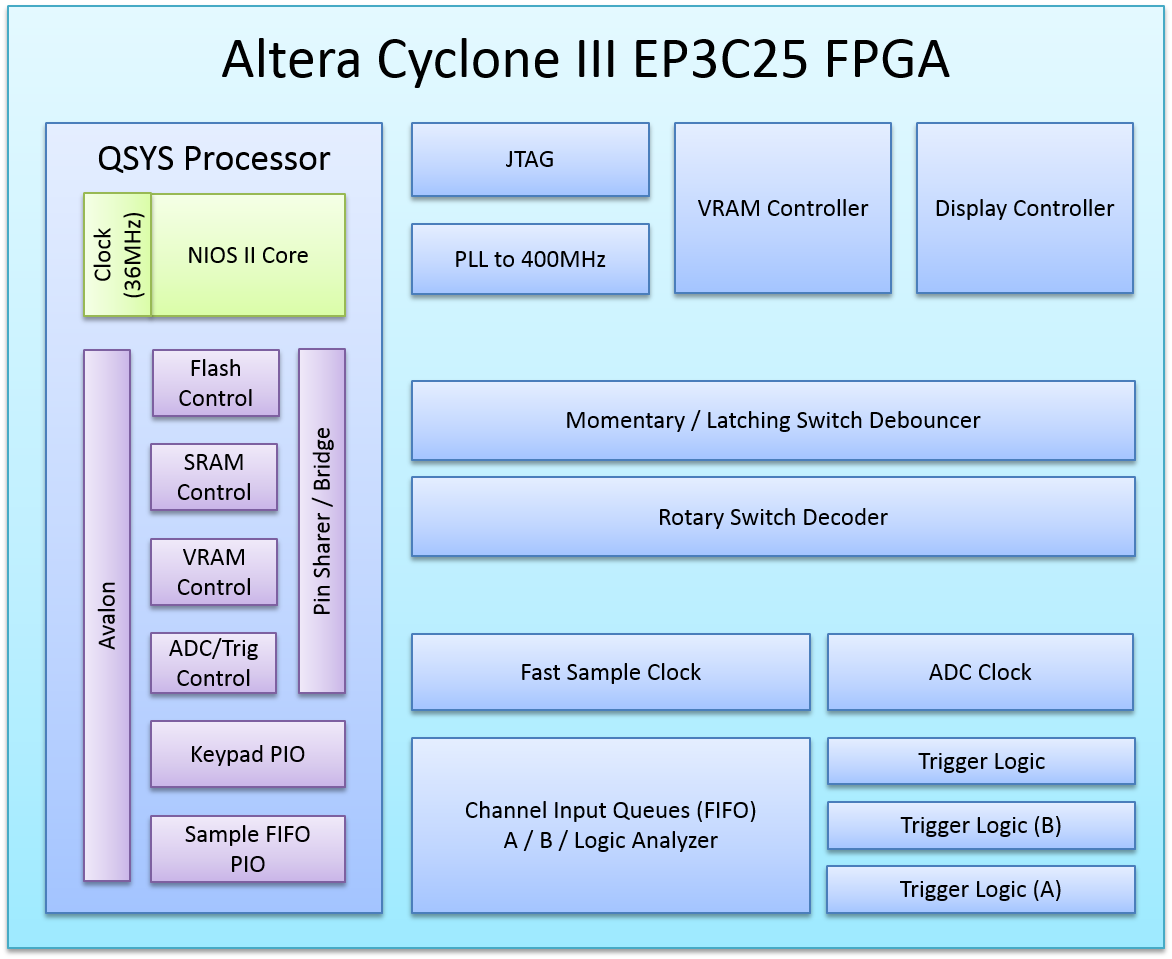
\includegraphics[width=3in]{block_diagrams/fpga.png}
		\caption{FPGA main components}
\end{figure}

Here's the major components of the FPGA logic. Most broadly, we have a NIOS II CPU, various clocks and timers, VRAM and display controllers, key debouncers and rotary encoder decoders, and finally, the scope sampling logic (FIFO storage, triggering, etc). We'll consider each of these in more detail.

\section{Clocks}

The system is fed an external $36MHz$ signal. This signal feeds direcly into some of the core logic, such as the NIOS II processor. However, in some cases we need a much faster (for sampling) or slower (for human-time-scale delays) clock signal.

\begin{figure}[ht!]
    \centering
    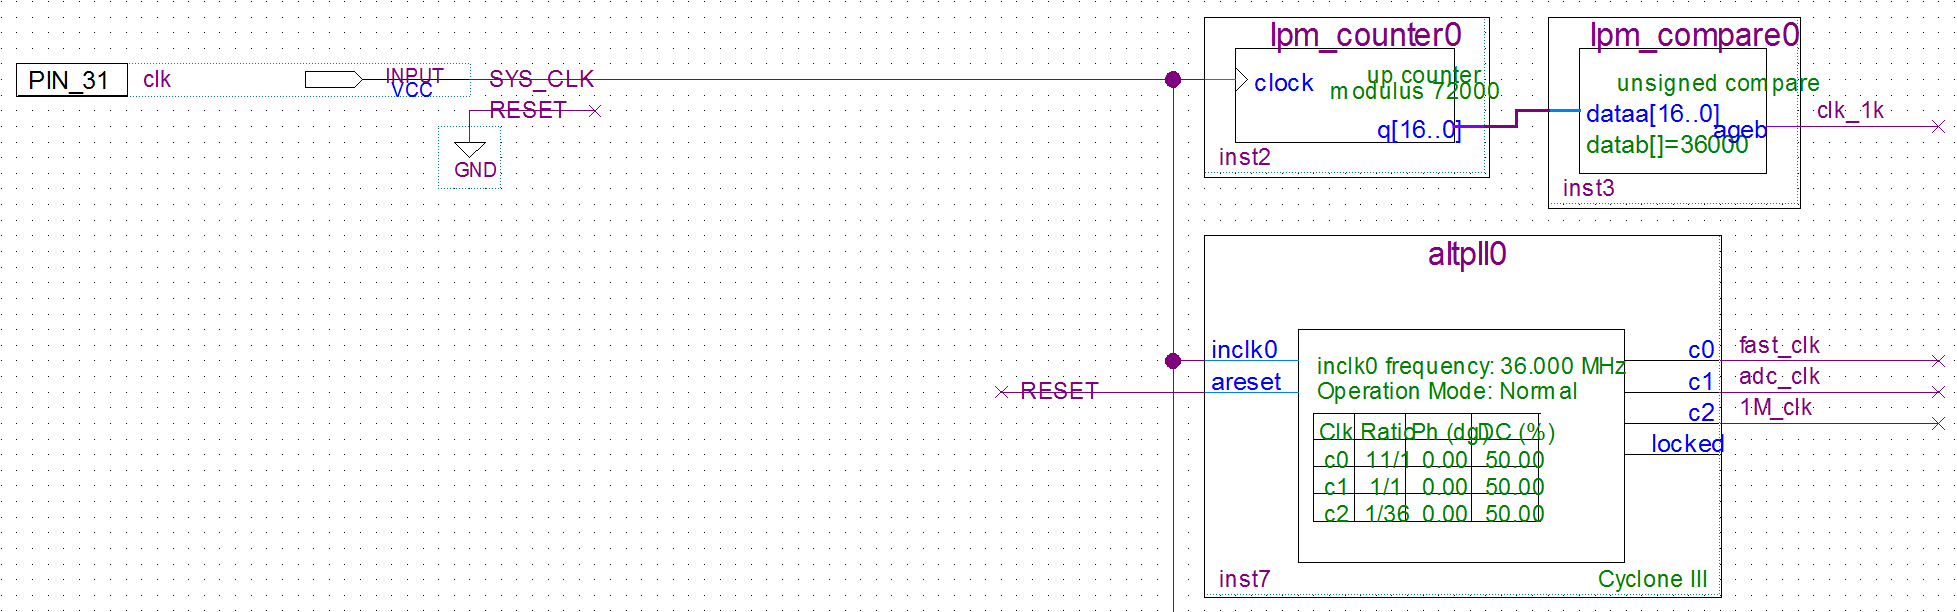
\includegraphics[width=6in]{fpga_logic/clocks.png}
		\caption{FPGA main clocks}
\end{figure}

A $50\%$ duty cycle $500Hz$ clock (incorrectly named \verb=clk_1k=) is produced by hooking a joint counter/compare to the $36Mhz$ signal. With a counter taken modulo $72,000$, incrementing at $36Mhz$ takes $2ms$. With a compare at $36,000$, we can then get a $50\%$ duty cycle $500Hz$ clock.

For the ADC and FIFO sampling, we want a much higher rate of about $400MHz$ (this is useful for the logic analyzer, even though the ADC can only produce new samples at $80MHz$). To do this, we use an phase-locked loop with an $11\times$ multiplier. This produces a $396MHz$ signal, close enough to $400MHz$. $400MHz$ was chosen because of its easy divisibility by factors of $2$ and $5$ (the common time scale factors used in scopes).

\begin{figure}[ht!]
    \centering
    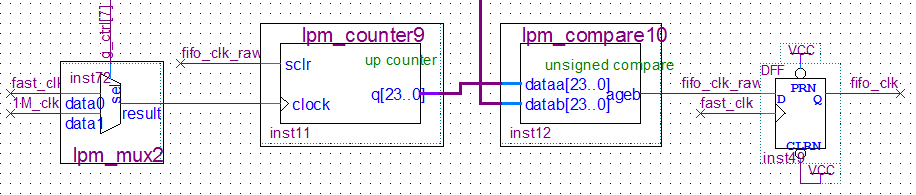
\includegraphics[width=6in]{fpga_logic/adc_sample_clk.png}
		\caption{FPGA sample clock}
\end{figure}

We need to be able to modify the rate at which we sample data in our code. To do this, we can attach a counter/compare to the fast $400MHz$ clock, and have the compare value set by the code. The logic above produces the sample clock. Notice that there are two selectable inputs to the counter/compre logic. One is the fast $400MHz$ clock for very high sample rates, and the other is a much slower $1MHz$ clock for slower sample rates. This is necessary because the $400MHz$ clock is less stable, especially with large counters such as a $32-bit$ counter, but has okay operating characteristics with the 24-bit one seen above.

\section{Sample Handling}

\begin{figure}[ht!]
    \centering
    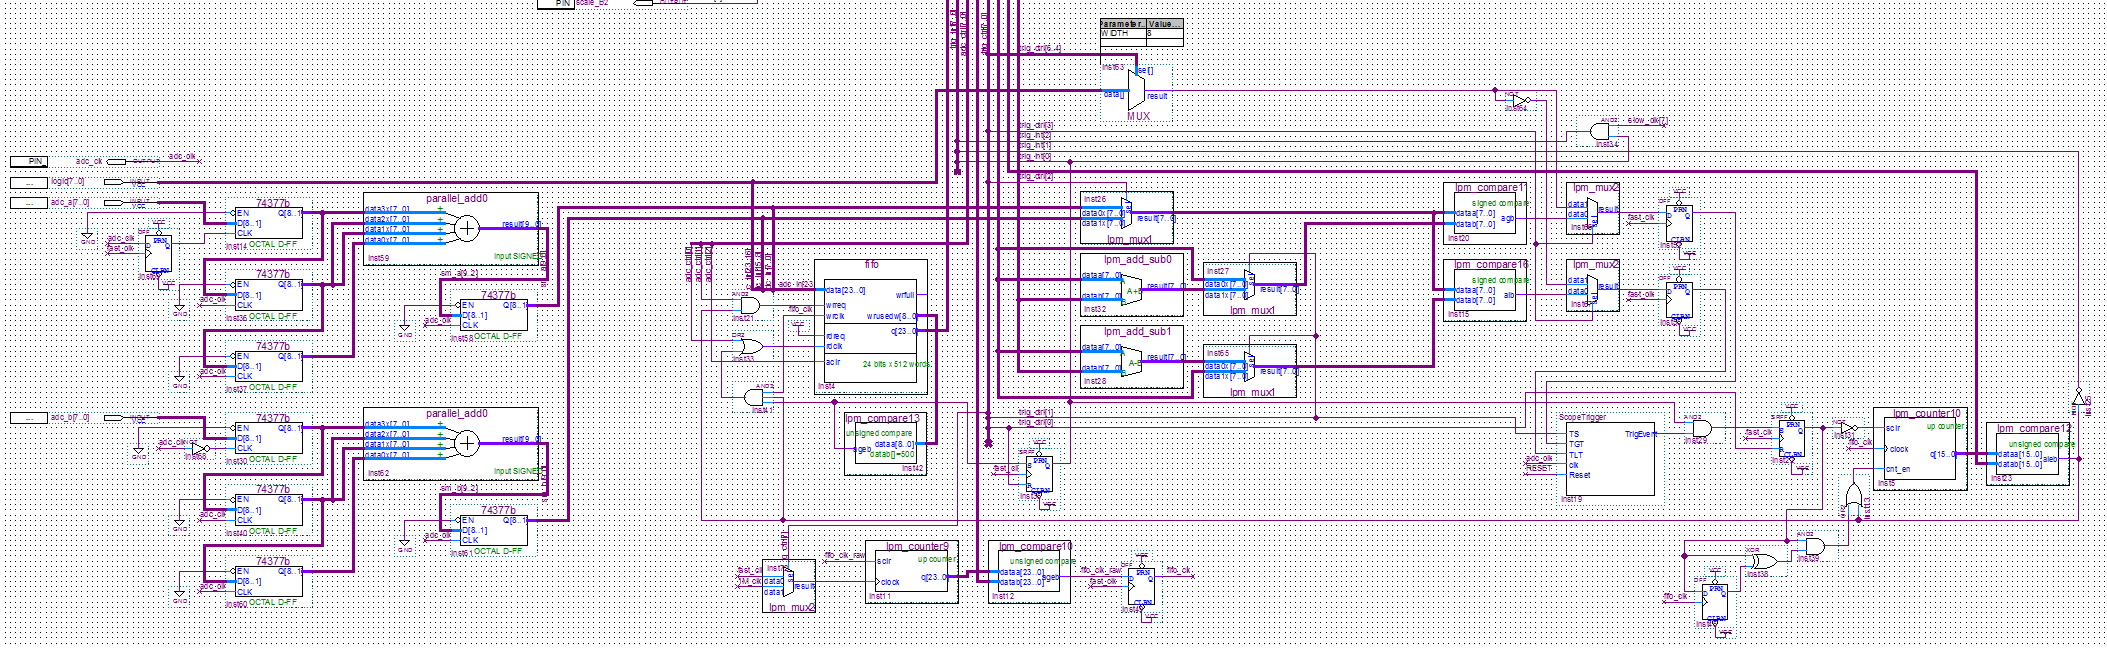
\includegraphics[width=6in]{fpga_logic/adc_overview.png}
		\caption{FPGA overview of scope sample handling}
\end{figure}

From left to right, we have the analog input logic, the sample FIFO and FIFO clock, and the trigger logic. We will look at each of these in detail.

\subsection{Analog Input}

The signal coming in from the ADC is somewhat noisy due to the suboptimal single-ended design of the analog frontend input to the ADC (it's designed for dual-ended input). Because of that, the signal can be a little noisy. To remedy this issue, the ADC signal is sent through a series of three 8-bit DFFs, and then a very simple 1D time-domain Gaussian blur is done on the signal.

\begin{figure}[ht!]
    \centering
    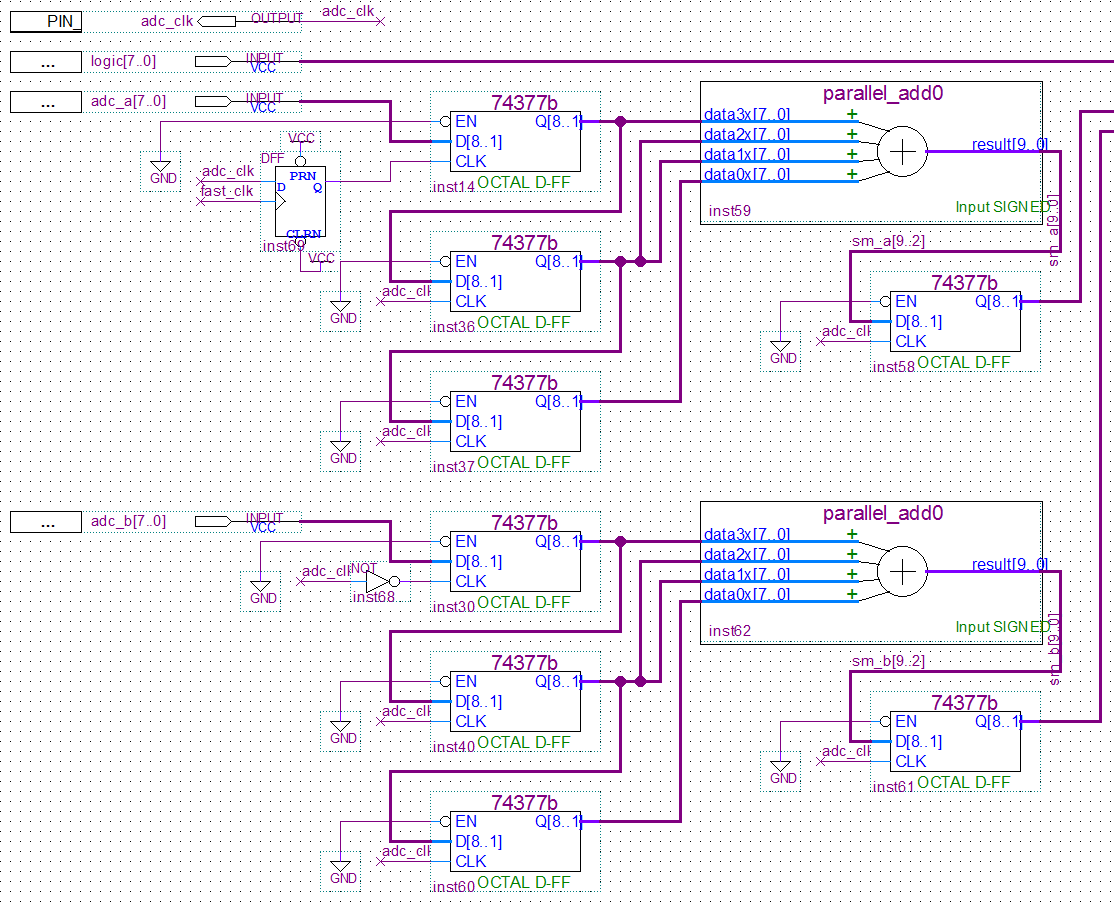
\includegraphics[width=5in]{fpga_logic/adc_input.png}
		\caption{FPGA sample input}
\end{figure}

Also notice that the first DFFs taking the ADC signal are offset by close to $180^o$ (in the top, there's a $\approx 2.5ns$ delay and in the bottom, a $\approx 12ns$ delay from the adc clock signal). This is because of how the ADC synchronizes its A and B channel outputs.

Output from the result of this logic is fed into the sample FIFO as well as the trigger logic.

\subsection{FIFO Sampling}

\begin{figure}[ht!]
    \centering
    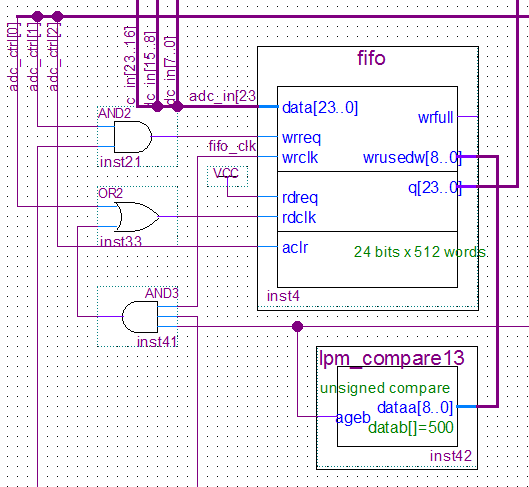
\includegraphics[width=2.5in]{fpga_logic/adc_fifo.png}
		\caption{FPGA sample FIFO}
\end{figure}

We are using a dual-clock FIFO in which data can be asynchronously written to (the back of the FIFO) and read from (the front of the FIFO) with different clocks. The way it's set up, the FIFO's write clock is based on the sample clock which can be as high as $400MHz$. Meanwhile, the read clock is bit-banged by the CPU when it wants to get the next 24 bits of data.

The FIFO logic is slightly complicated. First, when the FIFO fills, \verb=lpm_compare13= tells it to automatically start removing data (this allows the FIFO to act like a rotating buffer, always containing the last $N$ samples). Second, the FIFO stops collecting data automatically only when it sees a trigger event. Finally, the CPU has control over whether to allow reading and writing, and it can also clear the FIFO.

\subsection{Triggering}

\begin{figure}[ht!]
    \centering
    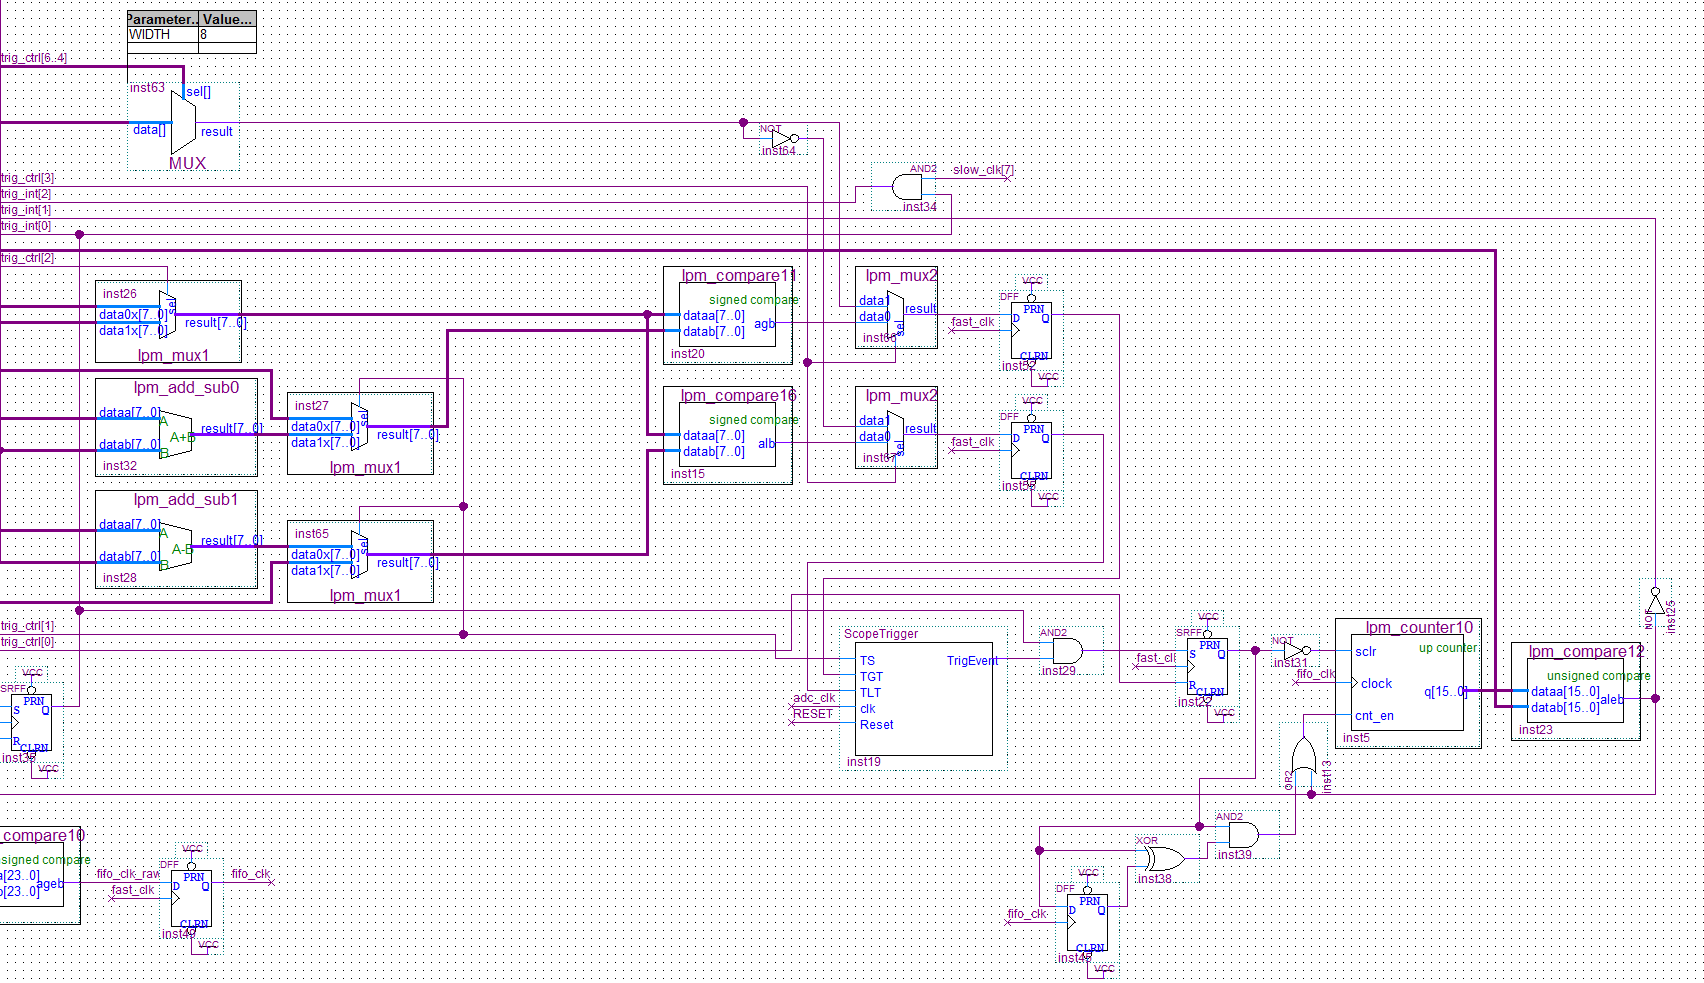
\includegraphics[width=6in]{fpga_logic/adc_trig.png}
		\caption{FPGA triggering}
\end{figure}

The function of this logic is to take the sample inputs and detect, using FPGA logic, when a given one of their values crosses a certain threshold, either in the positive or negative direction. This causes a trigger event which can automatically stop the sample FIFO after some specified delay. From here, the FPGA no longer accepts samples from the ADC or logic analyzer and the CPU can collect the FIFO samples. Once the CPU is finished, it can reset the FPGA logic to detect the next trigger event. The CPU provides information such as trigger channel, trigger level, trigger slope, and trigger error signals to control this section. It also provides a reset signal for when it's finished with the current trigger and wants the next one.

In the top left is a couple adders and MUXs. These take the desired trigger level and trigger error and produce dual outputs of the trigger level $\pm$ the trigger error. These outputs serve as upper and lower comparisons for the analog signal that's fed in through \verb=lpm_mux1= (which selects which analog channel to trigger on).

Above that is the logic analyzer input which also goes through a MUX to determine which bit (if any) to trigger on. From here, the compare results from \verb=lpm_compare11= and \verb=lpm_compare16= are MUXed with the logic analyzer and its inverse to select which of these signals we're interested in triggering against. Note that just as the analog signal has a lower and upper threshold, the logic analyzer can be fed as an upper threshold and the inverse of it as a lower threshold to provide identical thresholding functionality without requiring too much extra logic.

The selected trigger signals are cleaned with a DFF and then sent to the scope trigger state machine block which handles when to assert a trigger event based on the trigger thresholds \verb=TGT= and \verb=TLT= it sees, as well as the slope \verb=TS=. Once a trigger event is asserted, it sets an SRFF \verb=inst22=, which turns on counter \verb=lpm_counter10=. The logic below just turns off the counter before it loops over. This counter is responsible for the trigger delay, fed in by the CPU as a compare value for \verb=lpm_compare12=. Once the delay is over, the compare block outputs a high signal which sends an interrupt to the CPU and tells the FIFO to stop sampling data.

\subsection{Trigger State Machine}

\begin{figure}[ht!]
    \centering
    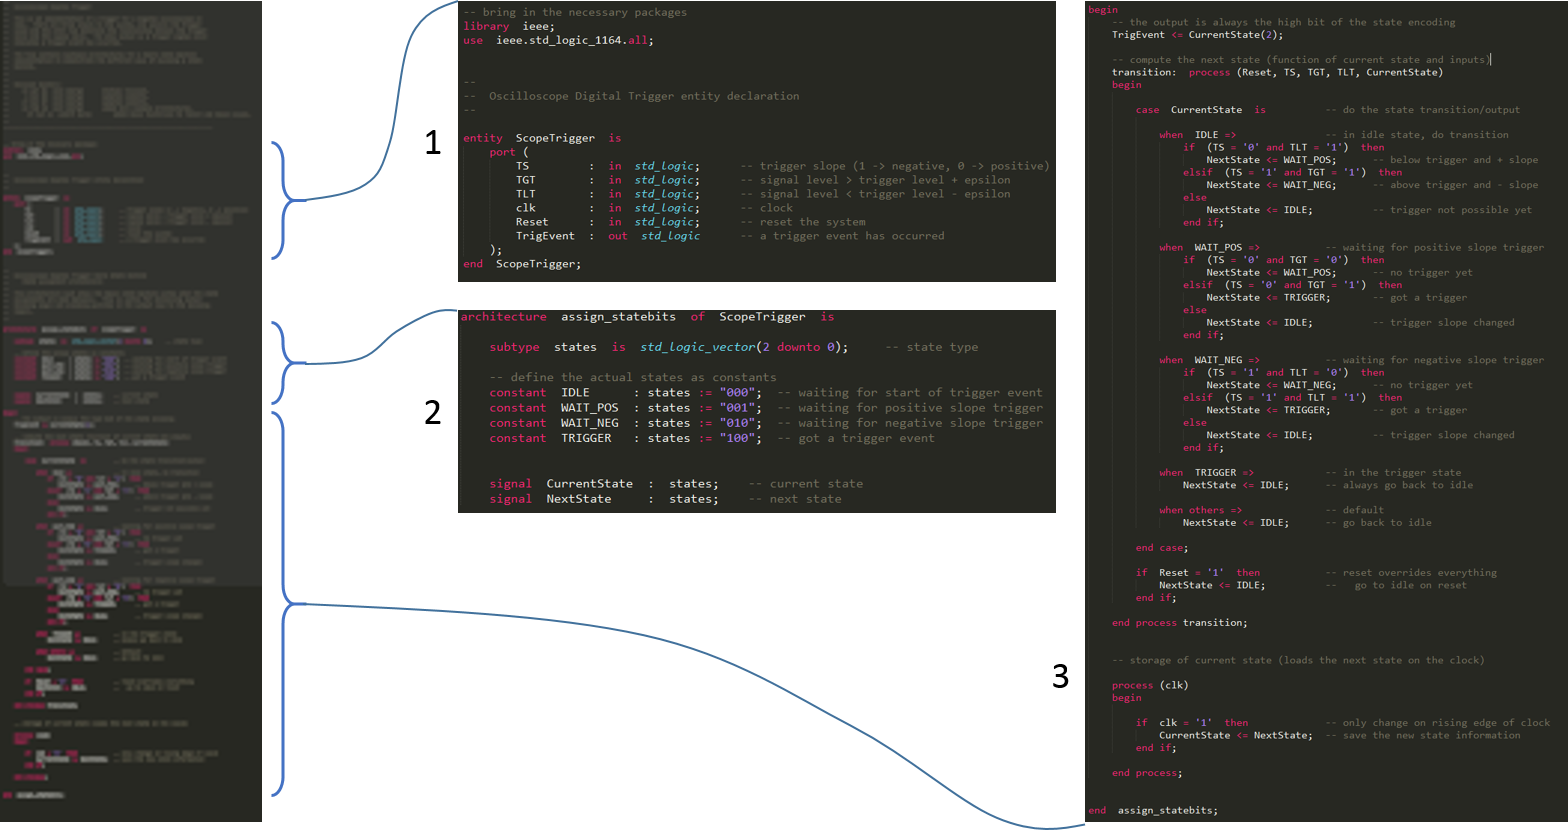
\includegraphics[width=6in]{fpga_logic/vhdl/triggering.png}
		\caption{FPGA triggering state machine}
\end{figure}

Shown above is the trigger state machine. It contains three main components, labeled above as (1) the input and output signals, (2) the states, and (3) the transitions. Operation is fairly straightforward and utilizes hysteresis on the two thresholded inputs. If \verb=TGT= goes from less than to greater than, then the signal just underwent a positive slope transition. The same goes for \verb=TLT= for negative slopes.

Notice that in the \verb=IDLE= state, it can only transition to \verb=WAIT_POS= after going below the lower threshold, whereas the upper threshold is needed to cause a trigger event. This is what allows for hysteresis. The same of course holds for \verb=WAIT_NEG=.

\section{VRAM and Display}

\begin{figure}[ht!]
    \centering
    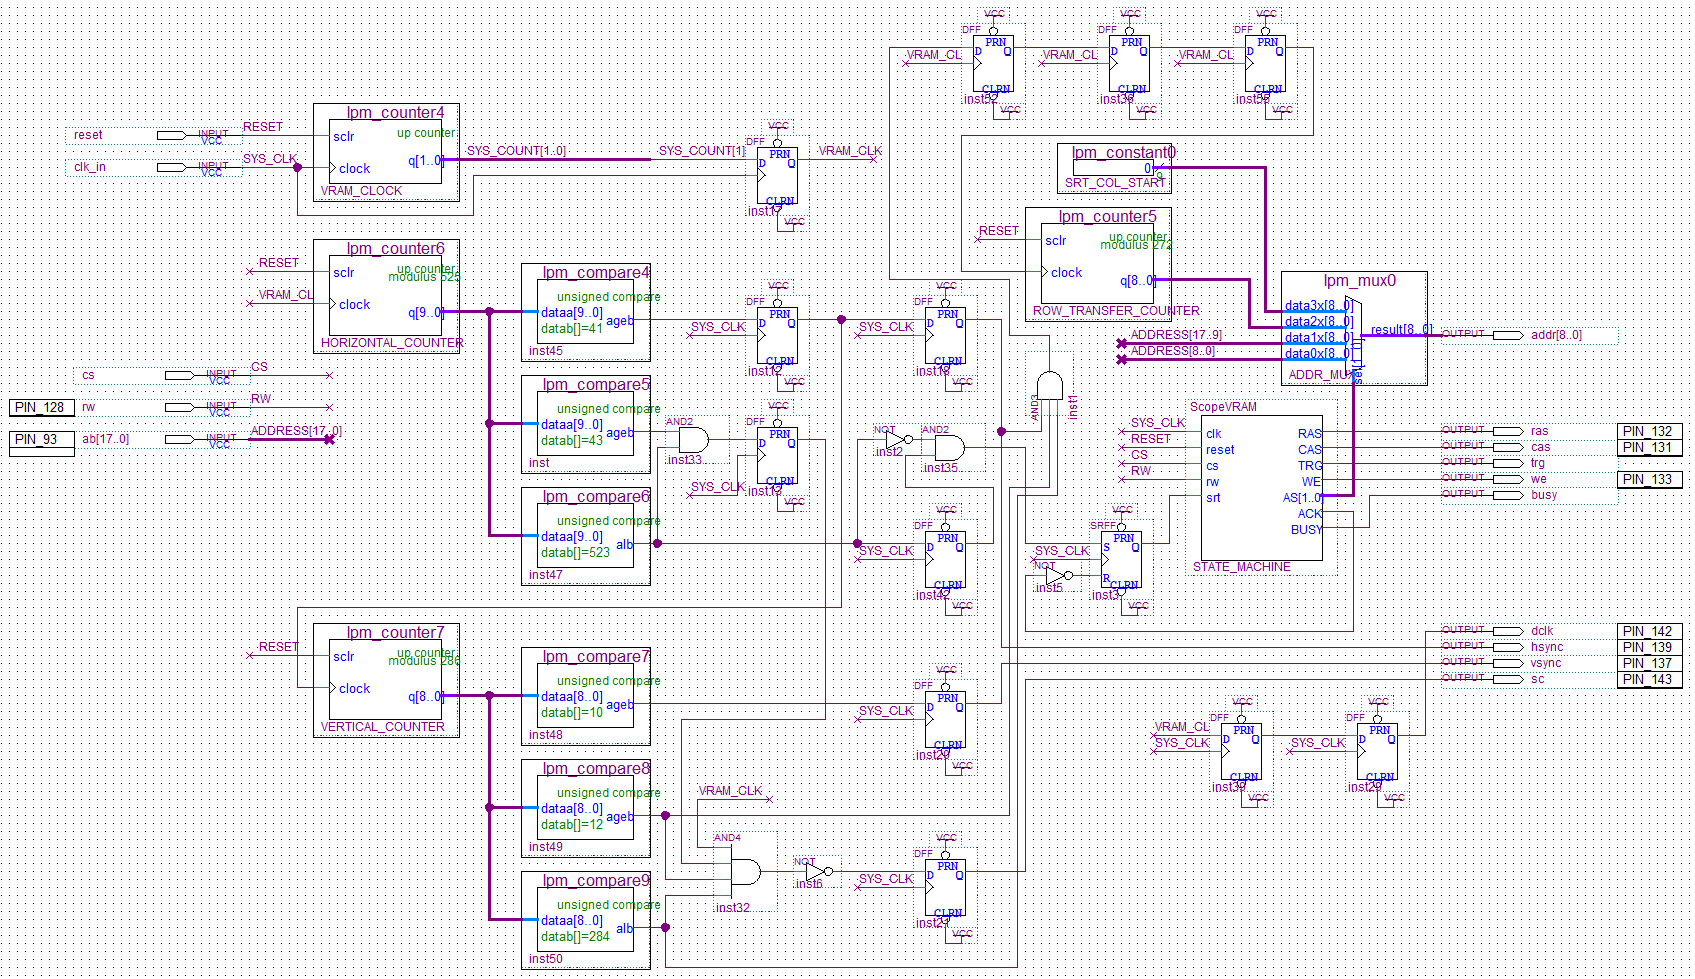
\includegraphics[width=6in]{fpga_logic/vram_disp_overview.png}
		\caption{FPGA overview of VRAM controller and display controller}
\end{figure}

The display and VRAM control logic are lumped together due to the similarities in requirements of their timing (although most of the VRAM control is handled by the state machine). Most of the logic seen above controls timing for the display clocks, while the portion in the upper right is for VRAM control. Much of the VRAM control logic shown here controls the 9-bit VRAM address output.

\subsection{VRAM Controller}

\begin{figure}[ht!]
    \centering
    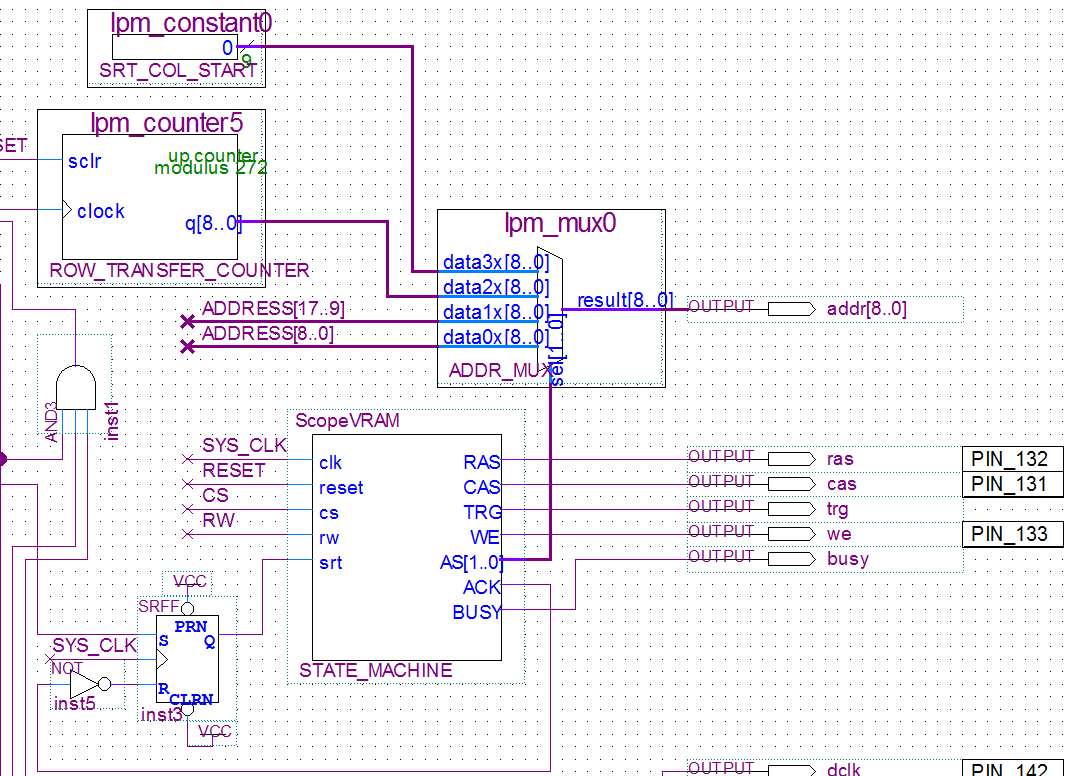
\includegraphics[width=3in]{fpga_logic/vram_disp_addr.png}
		\caption{FPGA VRAM addressing}
\end{figure}

The heart of the VRAM controller is the state machine \verb=ScopeVRAM=. It takes the typical memory outputs of the CPU (CS and RW) and uses that for much more advanced control to the VRAM chip. The state machine only returns a \verb=busy= signal to the CPU to indicate completion of the requested task.

Besides the state machine, the other logic useful for the VRAM controller is selecting the address to put out on the VRAM address bits. This is done by MUXing the two halves of the address bits along with a couple other address, controlled by the state machine. The two halves of the address bus are used for specifying row and column in a standard read to or write from the CPU. The other two address are used for serial row transfer cycles and specify the row (output of \verb=lpm_counter5=) and column to start at (\verb=SRT_COL_START=) for a row transfer. The counter is updated and the serial row transfer state triggered right after every row of pixels is written to the display (at the end of a HSYNC cycle).

\subsection{VRAM State Machine}

\begin{figure}[ht!]
    \centering
    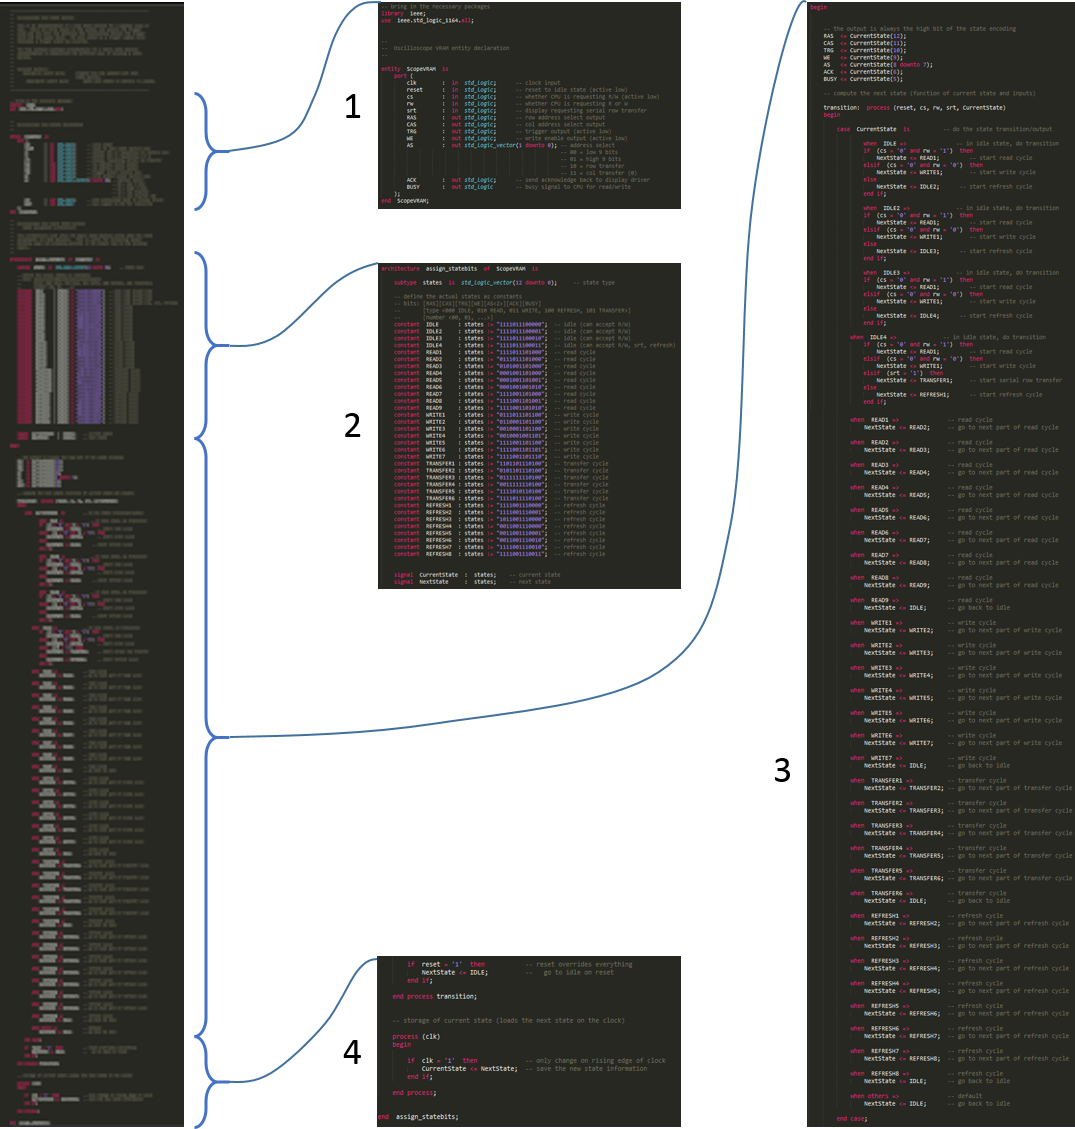
\includegraphics[width=6in]{fpga_logic/vhdl/vstates.png}
		\caption{FPGA VRAM controller state machine}
\end{figure}

The state machine is shown above. Just as in the triggering state machine, the VRAM state machine has (1) the inputs and outputs, (2) the states, and (3/4) the transitions. There are a lot of states, but their purpose is really to handle four main operations: read, write, refresh, and serial row transfer. In any given one of those desired operations, there are a number of states which run sequentially and handle the signal timing for the desired operation. In the transitions (3), you can see that the bulk of transitions move from a state in one operation to the next state in that operation (and at the end going back to \verb=IDLE=).

\subsection{Display Controller}

\begin{figure}[ht!]
    \centering
    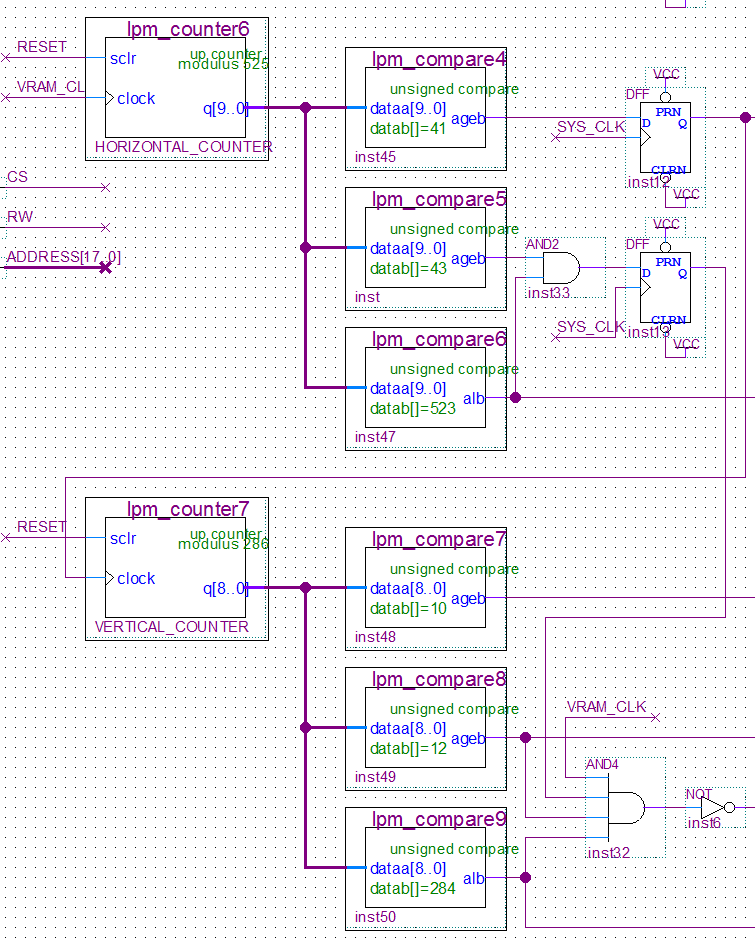
\includegraphics[width=3in]{fpga_logic/vram_disp_counters.png}
		\caption{FPGA display counter timers}
\end{figure}

Display timing is shown above. The \verb=VRAM_CLK= operates at about $9MHz$, approximately the dot clock frequency required by the display. \verb=lpm_compare4-6= then take care of a given HSYNC cycle - mainly the HSYNC pulse and the back and front porches. The HSYNC pulse in turn acts as a clock for the VSYNC counter. \verb=lpm_compare7-9= take care of a given VSYNC cycle - mainly the VSYNC pulse and the back and front porches.

\subsection{Display Timing (Testing)}

The tough timing requirements make testing a very good idea. Testing was done in Altera ModelSim with VHDL test code (provided in the appendix). To prove the importance of testing, here's an initial run of the display timing.

\begin{figure}[ht!]
    \centering
    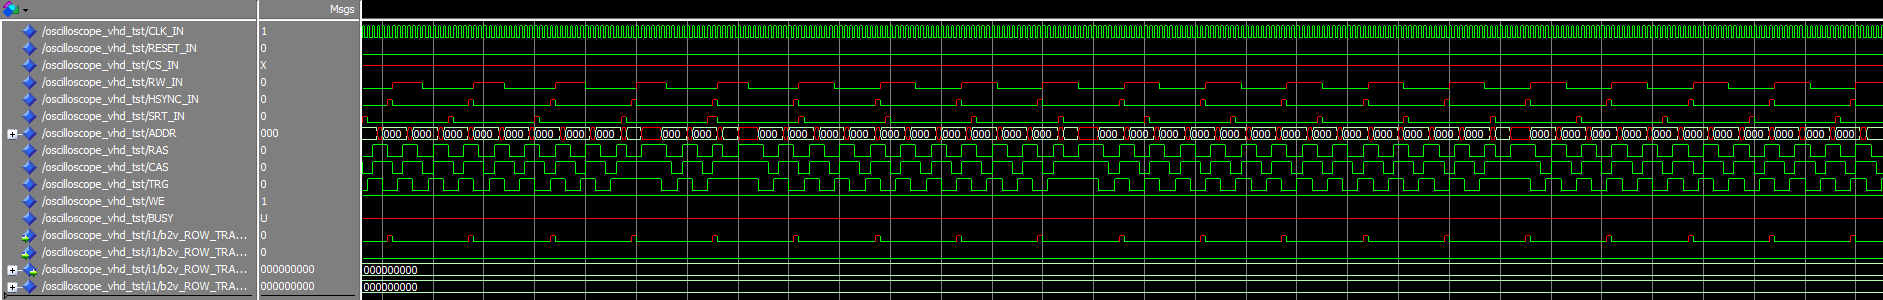
\includegraphics[width=4in]{timing/VRAM-test/vram-problem-start.png}
		\caption{Display timing test, problematic start}
\end{figure}

Notice that large portions of the signal are red, indicating there's a timing problem. In contrast, a successful run should have all green signals. Shown below is a semi-successful startup. The signals start out red due to a conflict in signal outputs (this was fixed), but then everything works properly.

\begin{figure}[ht!]
    \centering
    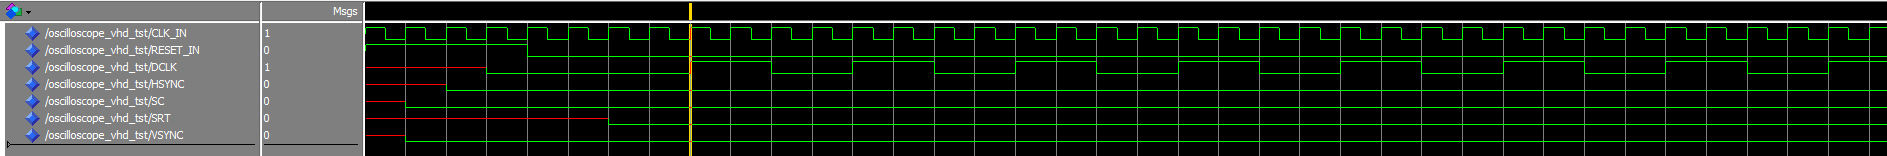
\includegraphics[width=6in]{timing/VRAM-test/display-success-start.png}
		\caption{Display timing test, semi-successful start}
\end{figure}

After fixing everything, all of the timing works out properly. Here are the signals at different zoom levels. First, looking at just the pulse of a horizontal cycle. Then looking at the full horizontal cycle. Then, looking at a pulse of a vertical cycle, and finally the full cycle (each period represents one full display refresh).

\begin{figure}[ht!]
    \centering
    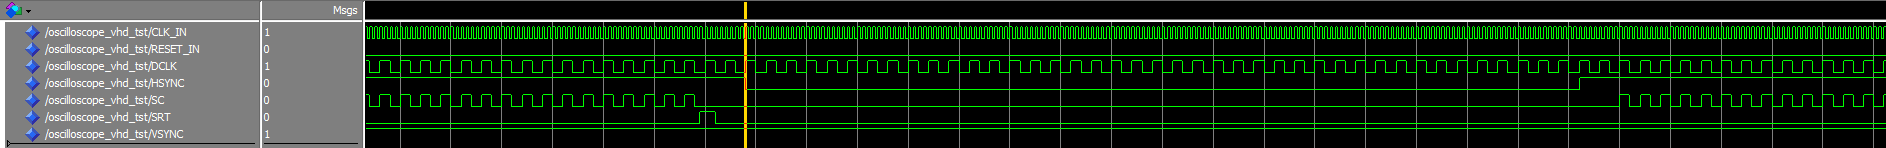
\includegraphics[width=6in]{timing/VRAM-test/display-success-horiz-pulse.png}
		\caption{Display timing test, successful horizontal pulse}
\end{figure}

\begin{figure}[ht!]
    \centering
    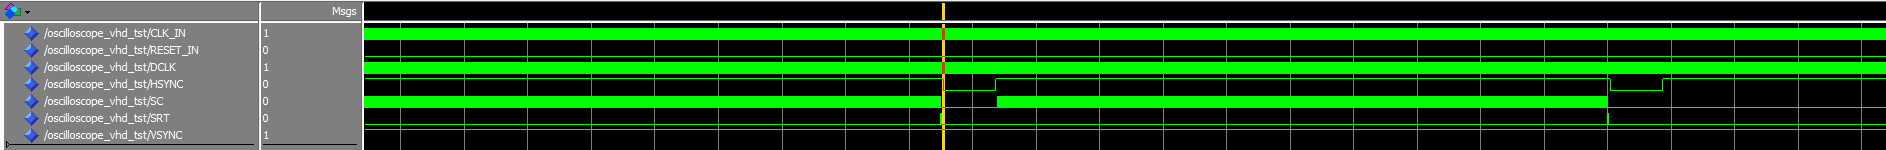
\includegraphics[width=6in]{timing/VRAM-test/display-success-full-horiz.png}
		\caption{Display timing test, successful horizontal cycle}
\end{figure}

\begin{figure}[ht!]
    \centering
    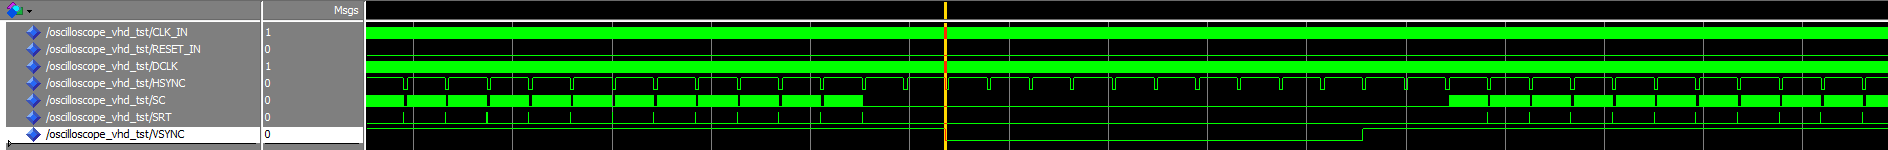
\includegraphics[width=6in]{timing/VRAM-test/display-success-vert-pulse.png}
		\caption{Display timing test, successful vertical pulse}
\end{figure}

\begin{figure}[ht!]
    \centering
    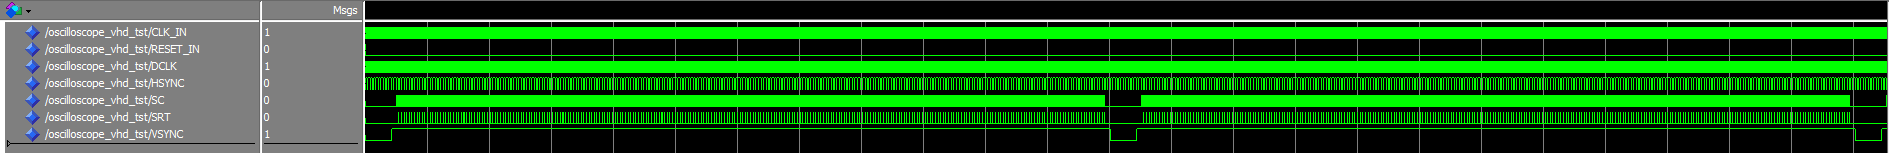
\includegraphics[width=6in]{timing/VRAM-test/display-success-full-vert.png}
		\caption{Display timing test, successful vertical cycle}
\end{figure}

We can see that the results are successful:

\begin{figure}[ht!]
    \centering
    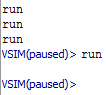
\includegraphics[width=1in]{timing/VRAM-test/display-success-full-output.png}
		\caption{Display timing test, all tests successful}
\end{figure}

\section{Switches}

All of the switch debouncing and decoding is done in FPGA logic. All of the switch-handling logic is shown here:

\begin{figure}[ht!]
    \centering
    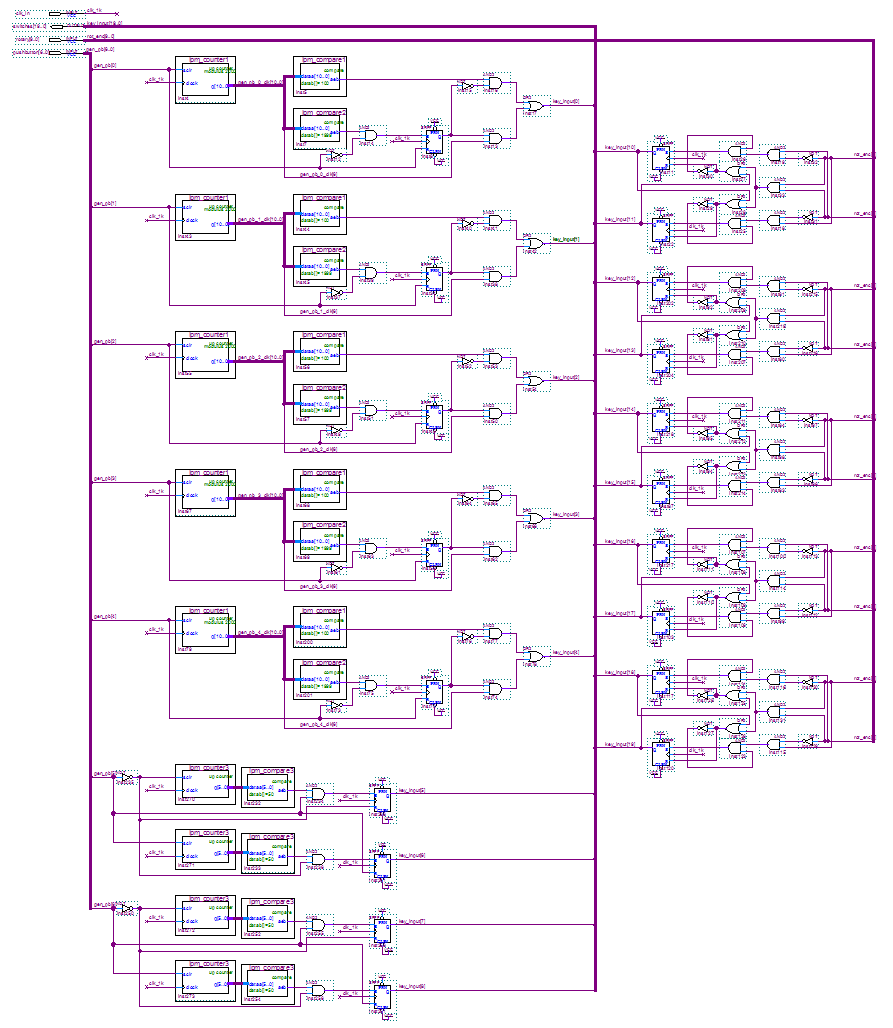
\includegraphics[width=6in]{fpga_logic/keys_overview.png}
		\caption{FPGA overview of key and rotary encoder input}
\end{figure}

The five display buttons are handled by logic in the top left, the two latching pushbuttons are handled in the bottom left, and the rotary decoding is handled by the five circuits on the right.

\subsection{Momentary Pushbutton Input}

The following logic circuit shows how the more basic momentary pushbuttons are debounced. When a pushbutton signal (active low) comes in, it unsets the counter clear, which allows the counter to start incrementing. If the button is pressed long enough without a bounce, then the counter will reach the first compare value, generating an interrupt for the CPU. If the switch continues being pressed, the second compare also kicks in and handles automatic switch repetition.

\begin{figure}[ht!]
    \centering
    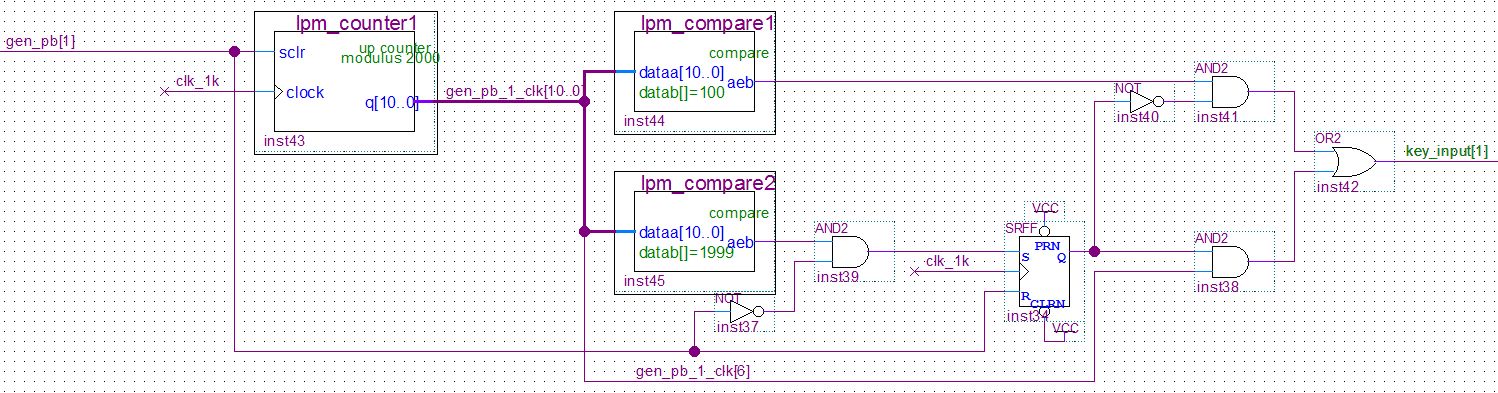
\includegraphics[width=6in]{fpga_logic/keys_pb.png}
		\caption{FPGA momentary pushbutton input debouncing}
\end{figure}

\subsection{Latching Pushbutton Input}

The latching pushbuttons are debounced in a similar manner to the momentary ones, with a counter/compare pair. However, there's no need for switch repetition. Instead, there's a need for debouncing the switch in both directions (hence the pair of counter/compares). Closing the pushbutton as well as openning the pushbutton will send separate interrupts to the CPU.

\begin{figure}[ht!]
    \centering
    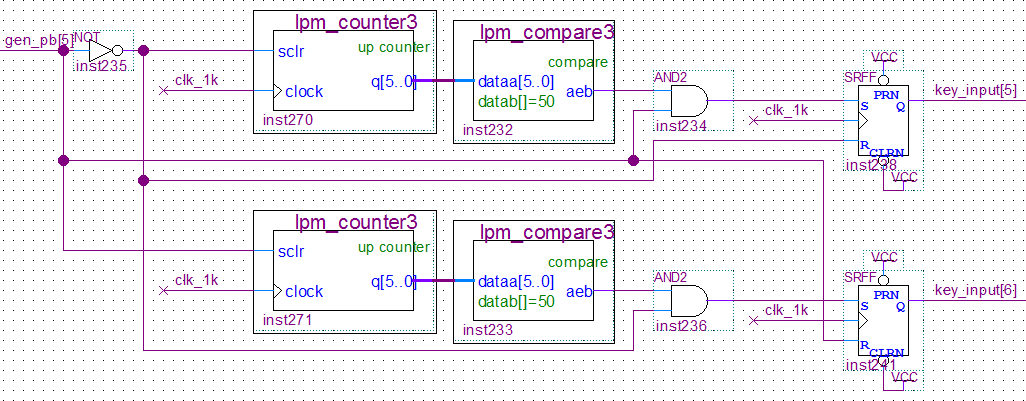
\includegraphics[width=6in]{fpga_logic/keys_pb_latching.png}
		\caption{FPGA latching pushbutton input debouncing}
\end{figure}

\subsection{Rotary Encoder Input}

At each detent of the rotary encoder, the A and B lines are held high. During a rotation by one detent, the A and B lines cycle through a grey code pattern depending on which direction the rotation was in. We can see this pattern in the diagram below. One way we can decode the signal, then, is to detect which of $\{A,B\}$ lines go low first (this indicates the rotation direction), and then wait for both of them to return high before going back to the initial state.

The diagram below shows the exact opposite polarity as what's described above, but the function is exactly the same.

\begin{figure}[ht!]
    \centering
    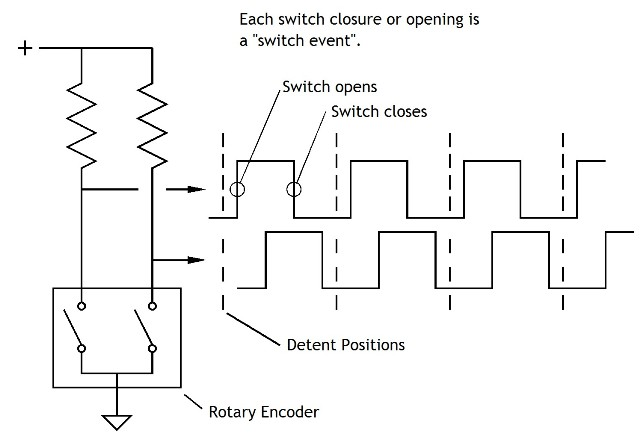
\includegraphics[width=3in]{Timing/encoder.jpg}
		\caption{Rotary encoder timing}
\end{figure}

We see that logic in the following circuit. In this circuit, the A and B rotary encoder lines come in from the right, and then interrupts for each of a CW or CCW turn are sent to the CPU on the left. We see the actual logic as described above. Whichever line falls low first sets the appropriate SRFF (triggering either a CW or CCW interrupt), and suppresses the other line from setting the opposing SRFF. Finally, the reset signal is generated when both lines go high again.

\begin{figure}[ht!]
    \centering
    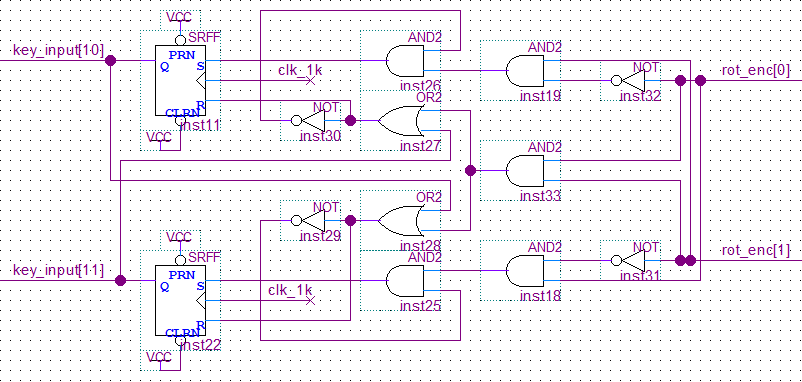
\includegraphics[width=6in]{fpga_logic/keys_rotary.png}
		\caption{FPGA rotary encoder decoding}
\end{figure}

\newpage
\section{NIOS II Processor}

\begin{figure}[ht!]
    \centering
    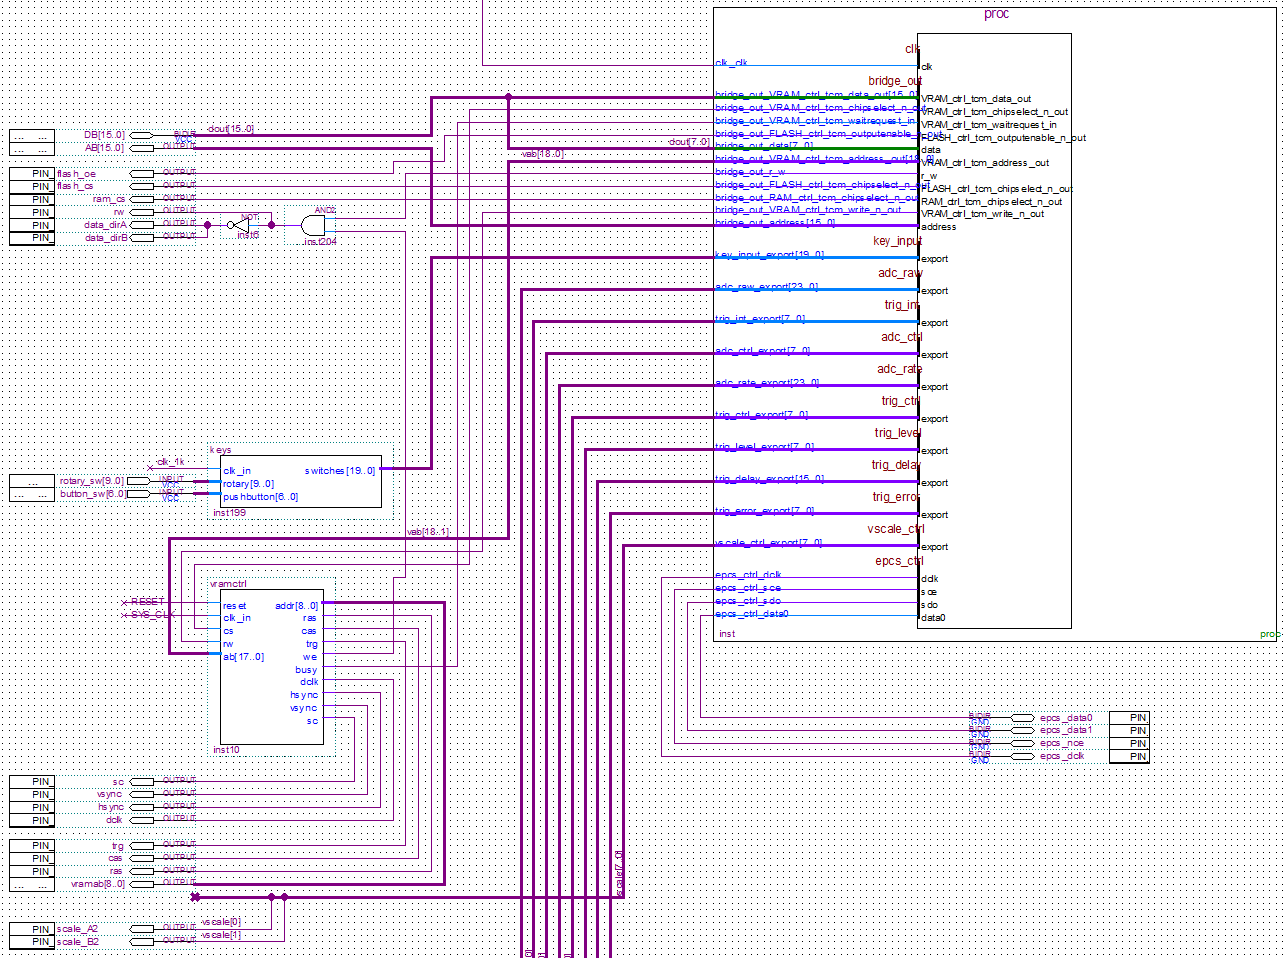
\includegraphics[width=6in]{fpga_logic/proc_overview.png}
		\caption{FPGA NIOS II processor block}
\end{figure}

The Altera Cyclone III FPGAs have enough logic gates to support a simple processor, called the NIOS II. It has a RISC architecture with 32 registers and a small instruction set. More information about the NIOS II can be found online.

In the circuit above, the processor and some core peripherals are shown in a single block at the top right. It interfaces with FPGA I/O (at the left of the schematic), as well as the key and VRAM control modules (middle left), EPCS (bottom right), and triggering logic (not shown, below).

\subsection{Overview of Capabilities}
\begin{figure}[ht!]
    \centering
    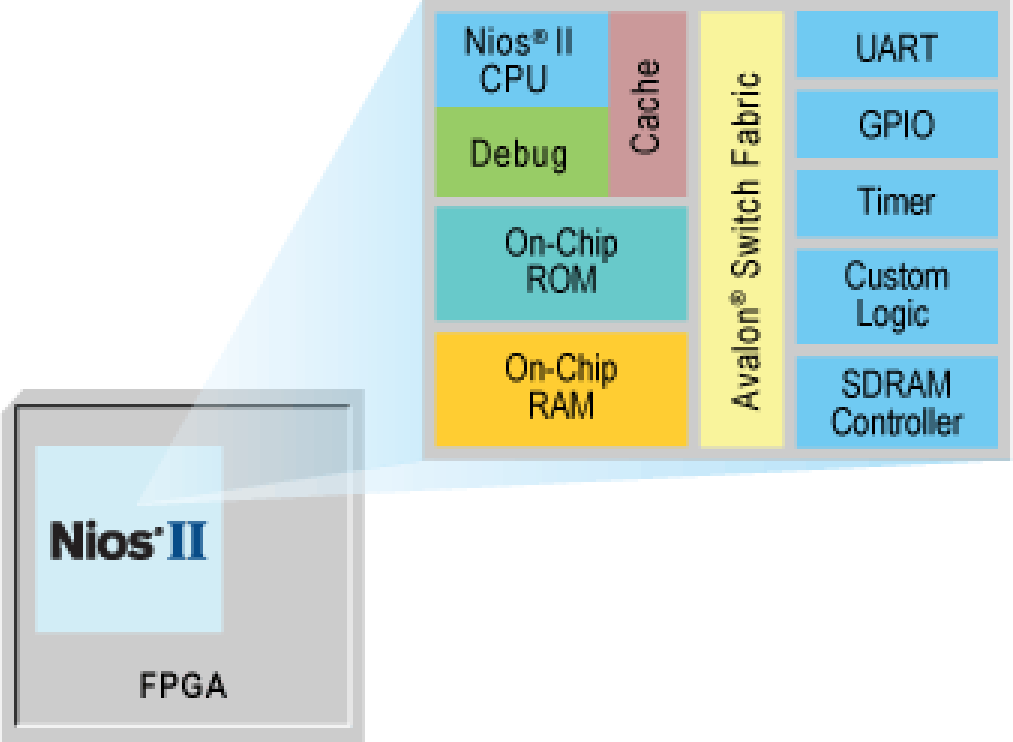
\includegraphics[width=2in]{images/nios_ii.png}
		\caption{NIOS II soft core processor}
\end{figure}

The processor can be built up using the a subtool of Quartus called QSYS. This system can be used to create not only the core NIOS processor, but also supporting components such as an Avalon bus for managing peripherals, interrupts, input and output to the CPU, etc.

Once the processor is designed in QSYS, it can be generated into a block for use in the logic circuit. In a block diagram file, all inputs/outputs exported in the QSYS screen can be hooked up directly to the other FPGA logic. This allows for seamless integration of the FPGA logic and the soft core CPU.

\subsection{Peripherals}

In addition to the basic NIOS II processor and clock, there are a number of peripherals we can add.

For memory modules which share signals to the outside world, we do this with a Generic Tri-State Controller for each memory module, a Tri-State Conduit Pin Sharer to share certain connections/buses, and finally a Tri-State Conduit Bridge takes the shared symbols and exports them as pins on the processor block.

For simple inputs/outputs between the processor and the outside world, a simple Parallel I/O peripheral can be used. These PIOs can be configured as input, output, and bidirectional. Inputs can trigger interrupts.

\begin{figure}[ht!]
    \centering
    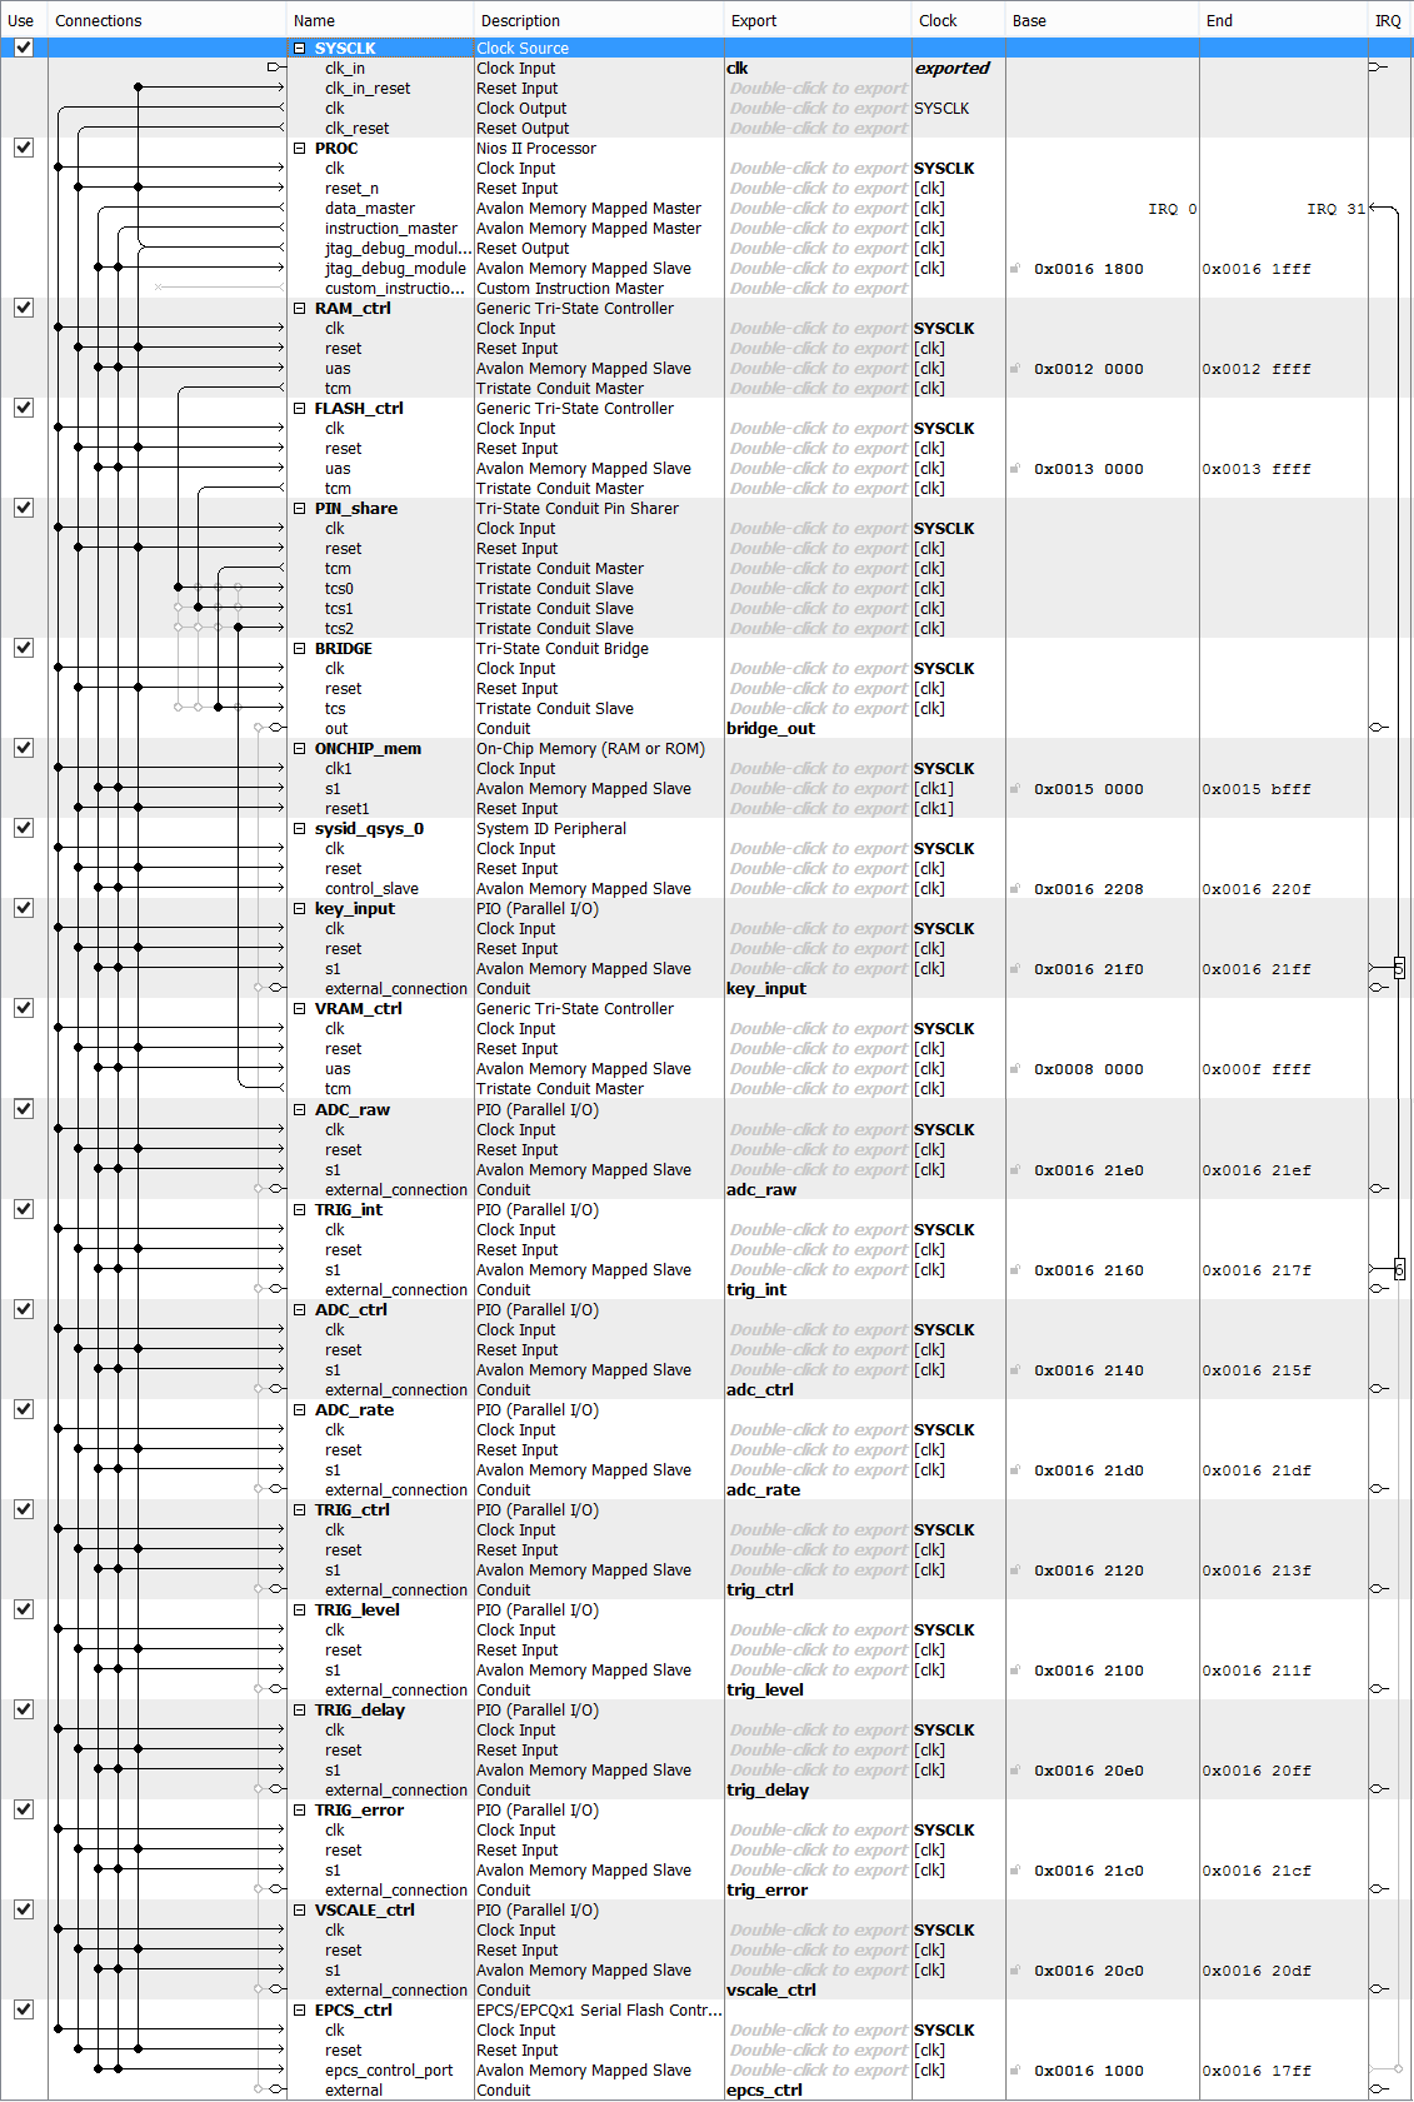
\includegraphics[width=4in]{fpga_logic/proc_periph.png}
		\caption{NIOS II core peripherals}
\end{figure}

\subsection{NIOS II Settings}

These are the settings for the NIOS II processor. We're using the NIOS II/s version, which includes instruction caching and hardware divides. Caching is particularly important. Without caching, the processor runs much slower and the LCD refresh rate is very noticeable.

\begin{figure}[ht!]
    \centering
    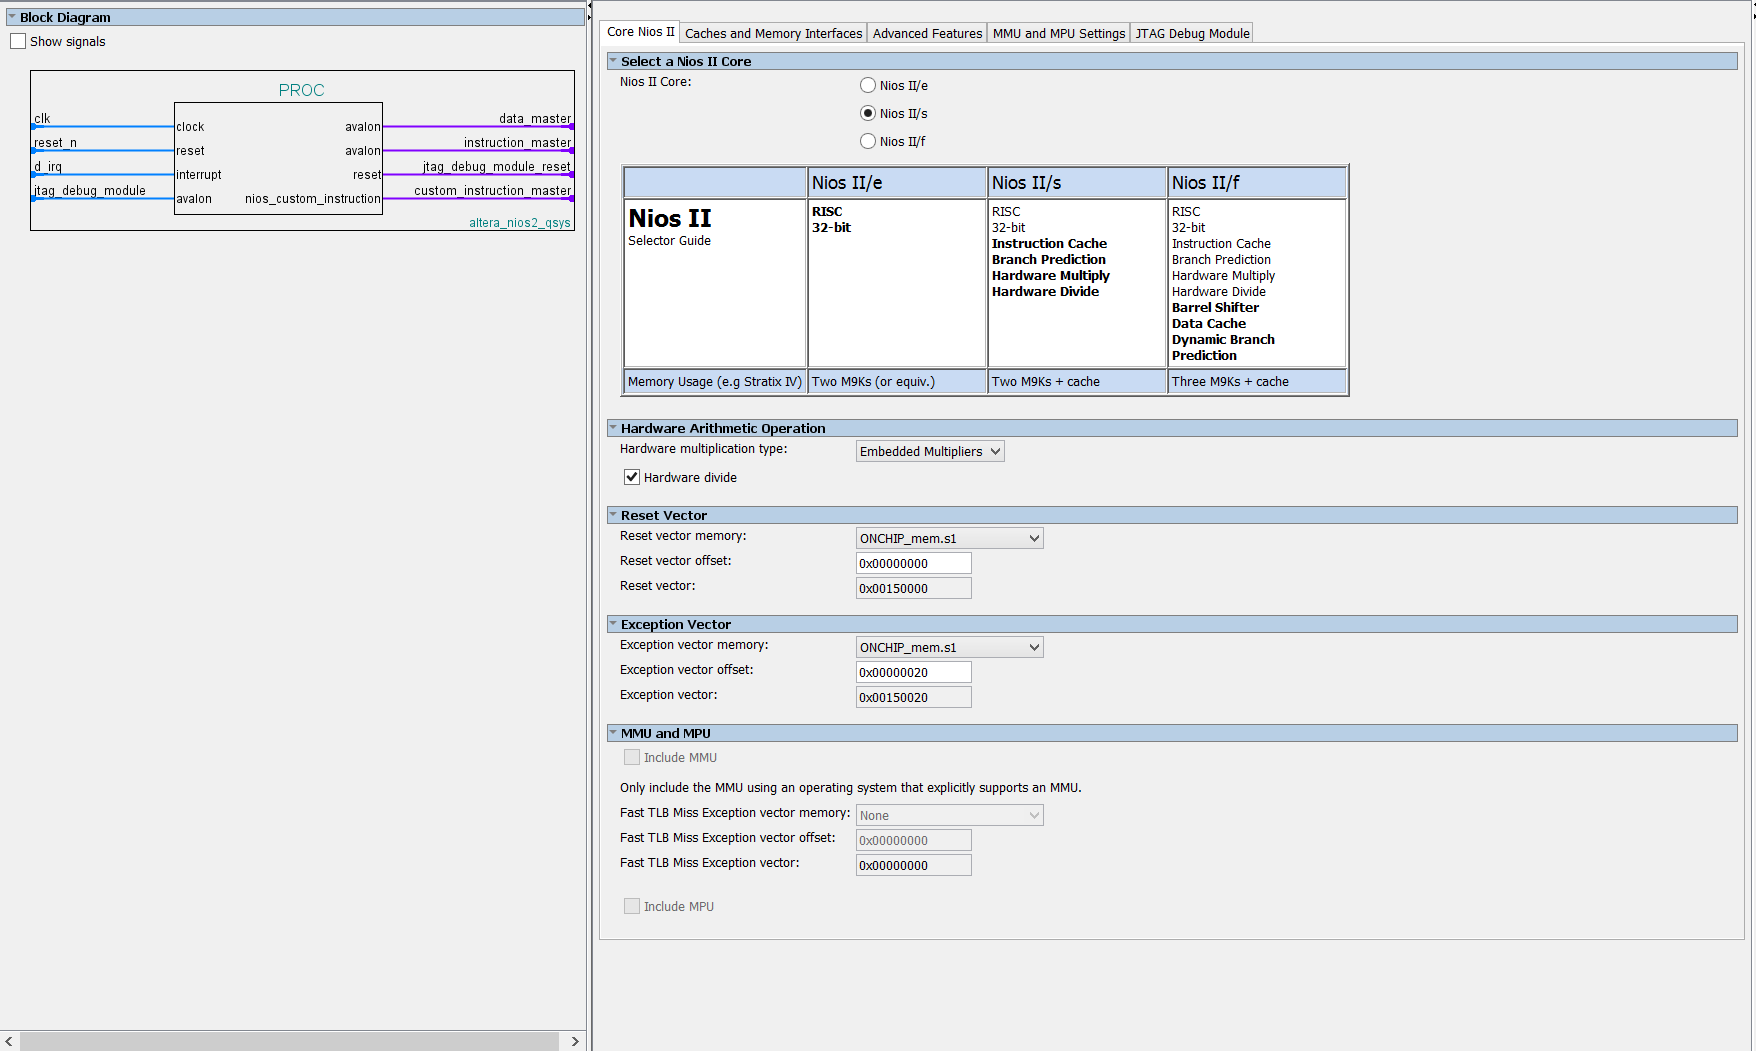
\includegraphics[width=4in]{fpga_logic/proc_settings.png}
		\caption{NIOS II core settings}
\end{figure}

\subsection{Address Memory Map}

Finally, with this whole QSYS processor setup, we can generate the addresses for each component, seen below. Once that's done, we generate the entire processor (VHDL file, as well as a block diagram block). Configuration details about the base addresses (including \verb=#define=s) of each of these peripherals is included in the generated processor files. This can be used in the NIOS II code to allow for easy maintenance of the NIOS code, agnostic to changes in the actual base addresses.

\begin{figure}[ht!]
    \centering
    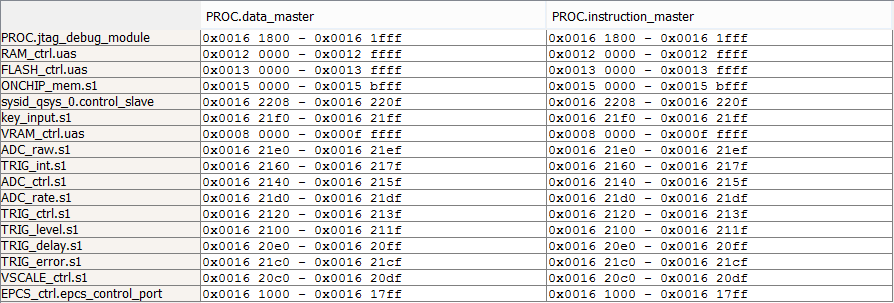
\includegraphics[width=6in]{fpga_logic/address_map.png}
		\caption{NIOS II address memory map}
\end{figure}


\chapter{Software}\label{software}
\section{High-level Block Diagram}

\section{User Interface}

\section{Key Input}

\section{ADC / Sampling Input}

\section{Display Controller}

\section{Display Graphics}

\section{Testing}

\subsection{ADC}

\subsection{Keys}

\subsection{RAM}

\subsection{ROM}

\subsection{VRAM}

\subsection{Display}



%% <== End of hints
%%%%%%%%%%%%%%%%%%%%%%%%%%%%%%%%%%%%%%%%%%%%%%%%%%%%%%%%%%%%%



%%%%%%%%%%%%%%%%%%%%%%%%%%%%%%%%%%%%%%%%%%%%%%%%%%%%%%%%%%%%%
%% BIBLIOGRAPHY AND OTHER LISTS
%%%%%%%%%%%%%%%%%%%%%%%%%%%%%%%%%%%%%%%%%%%%%%%%%%%%%%%%%%%%%
%% A small distance to the other stuff in the table of contents (toc)
\addtocontents{toc}{\protect\vspace*{\baselineskip}}

%% The Bibliography
%% ==> You need a file 'literature.bib' for this.
%% ==> You need to run BibTeX for this (Project | Properties... | Uses BibTeX)
%\addcontentsline{toc}{chapter}{Bibliography} %'Bibliography' into toc
%\nocite{*} %Even non-cited BibTeX-Entries will be shown.
%\bibliographystyle{alpha} %Style of Bibliography: plain / apalike / amsalpha / ...
%\bibliography{literature} %You need a file 'literature.bib' for this.

%% The List of Figures
\clearpage
\addcontentsline{toc}{chapter}{List of Figures}
\listoffigures

%% The List of Tables
\clearpage
\addcontentsline{toc}{chapter}{List of Tables}
\listoftables


%%%%%%%%%%%%%%%%%%%%%%%%%%%%%%%%%%%%%%%%%%%%%%%%%%%%%%%%%%%%%
%% APPENDICES
%%%%%%%%%%%%%%%%%%%%%%%%%%%%%%%%%%%%%%%%%%%%%%%%%%%%%%%%%%%%%
%\appendix
%% ==> Write your text here or include other files.
\begin{appendices}

\chapter{Block Diagrams} \label{App:blockdiagrams}

\begin{figure}[ht!]
    \centering
    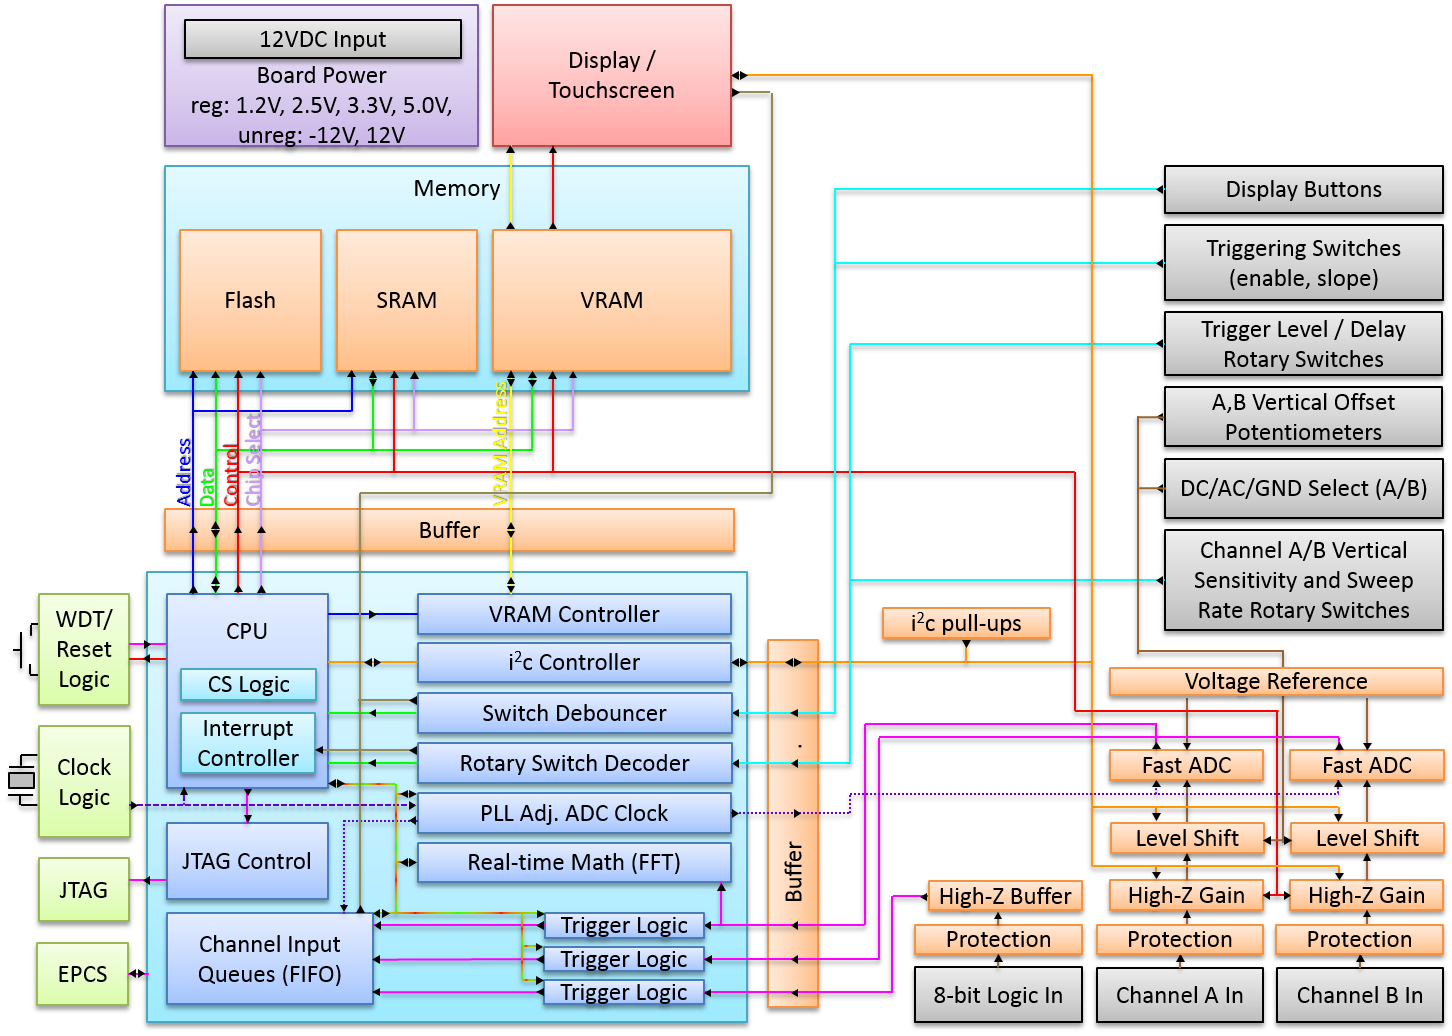
\includegraphics[width=6in]{block_diagrams/full.png}
		\caption{Full block diagram}
\end{figure}

\begin{figure}[ht!]
    \centering
    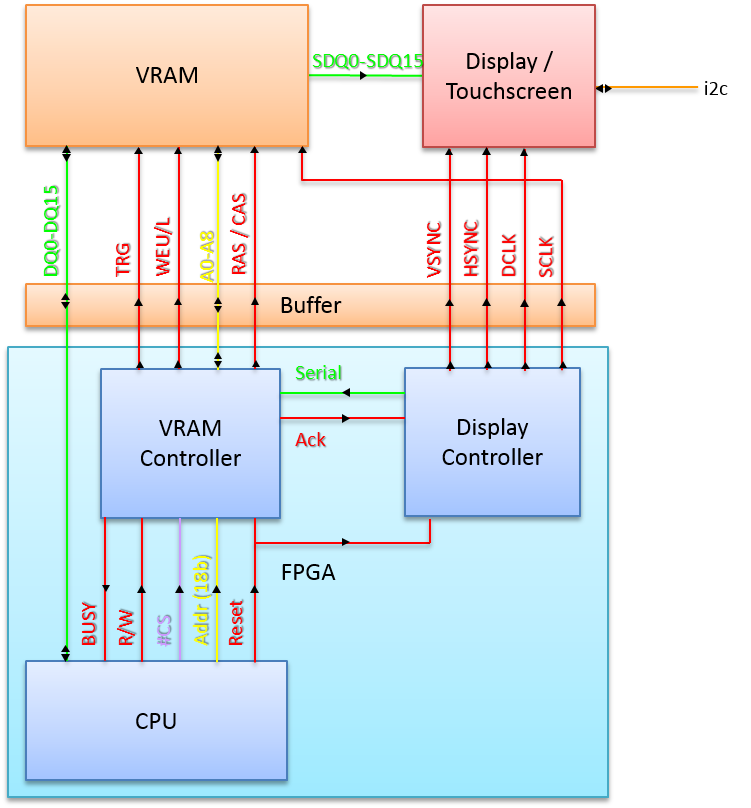
\includegraphics[width=3in]{block_diagrams/video.png}
		\caption{Display block diagram}
\end{figure}

\begin{figure}[ht!]
    \centering
    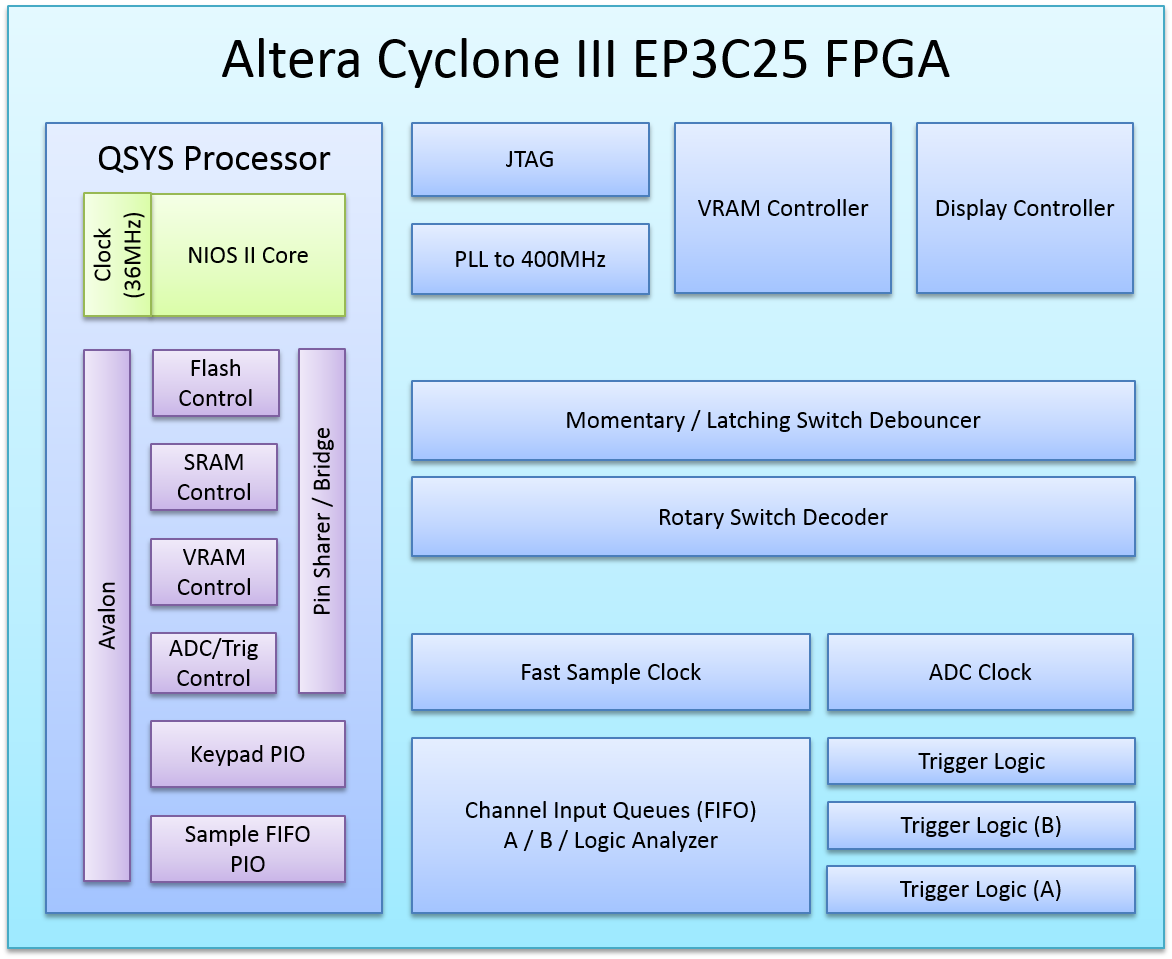
\includegraphics[width=3in]{block_diagrams/fpga.png}
		\caption{FPGA main components}
\end{figure}

\chapter{Schematic Diagrams} \label{App:schematicdiagrams}

\begin{figure}[ht!]
    \centering
    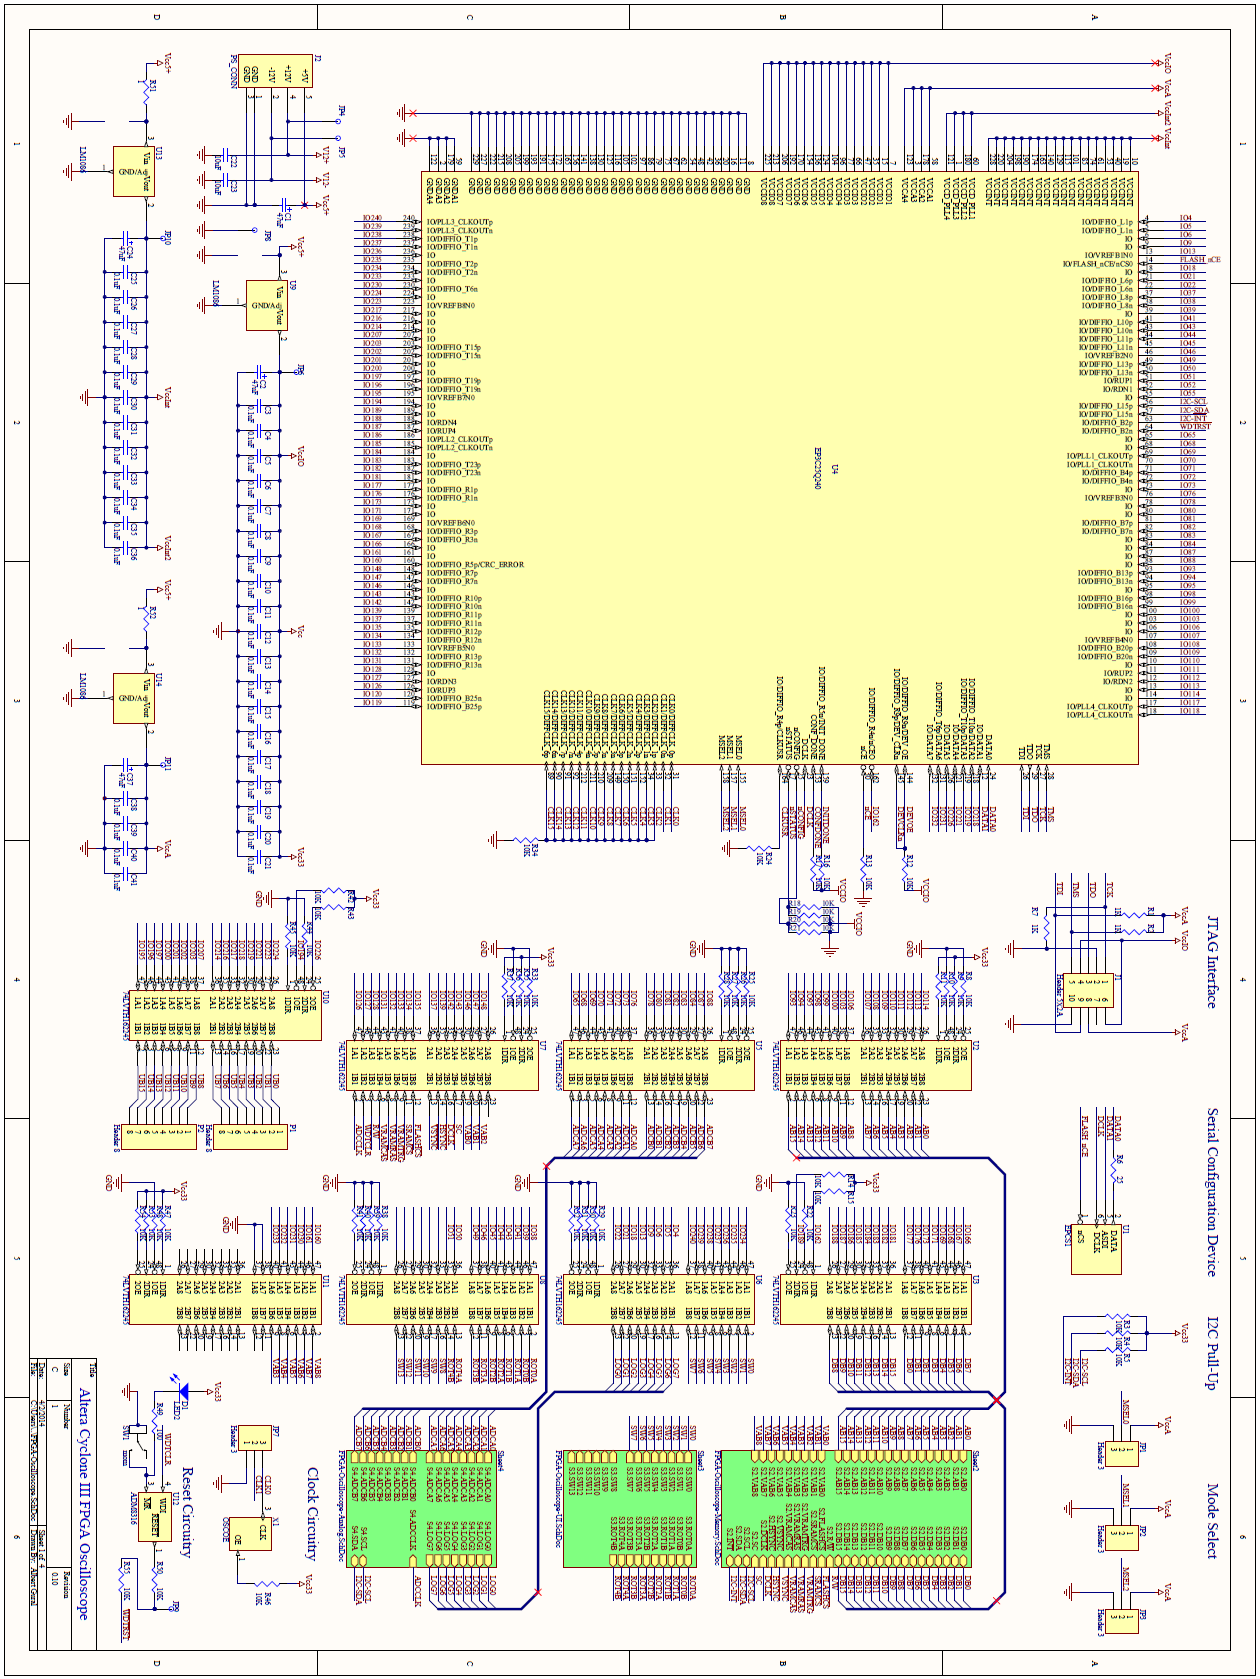
\includegraphics[width=6in]{circuit/main_fpga_page.png}
		\caption{FPGA and supporing components schematic diagram}
\end{figure}

\begin{figure}[ht!]
    \centering
    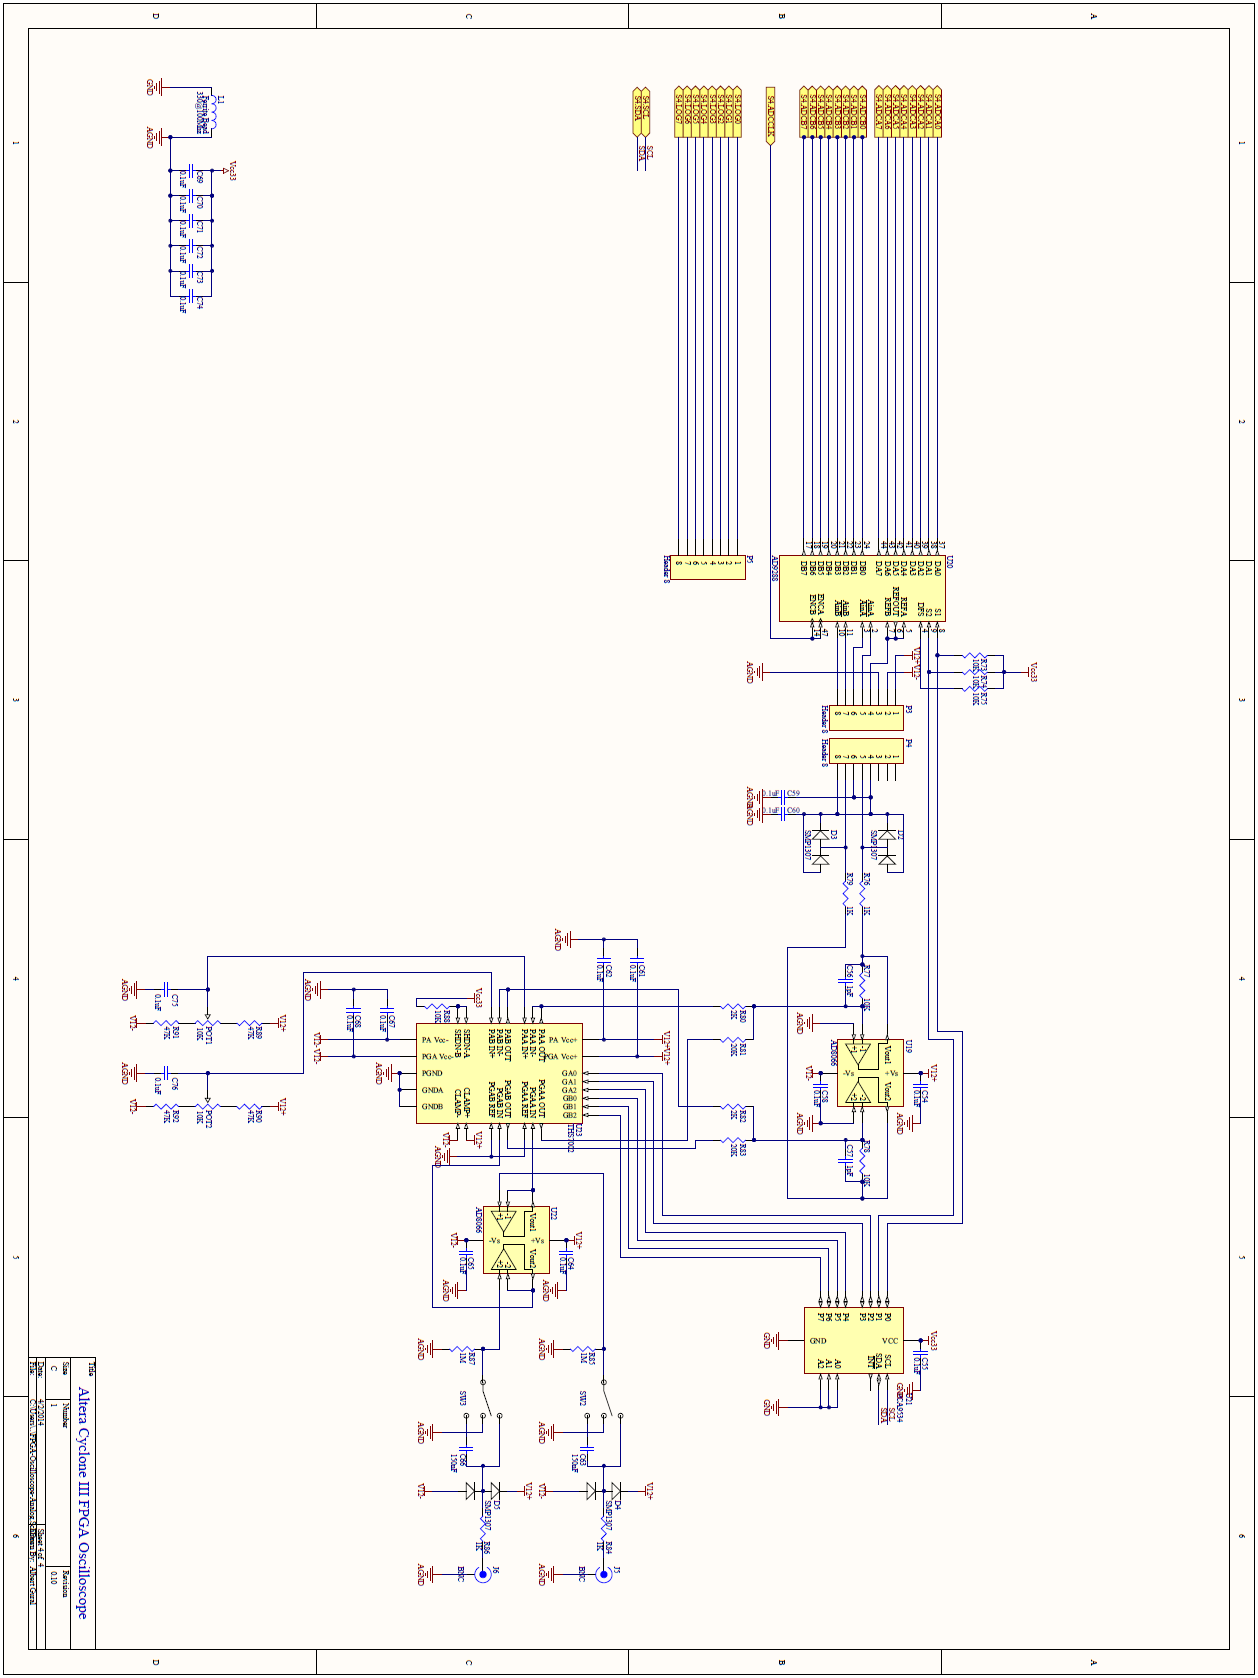
\includegraphics[width=6in]{circuit/analog_page.png}
		\caption{Analog section schematic diagram}
\end{figure}

\begin{figure}[ht!]
    \centering
    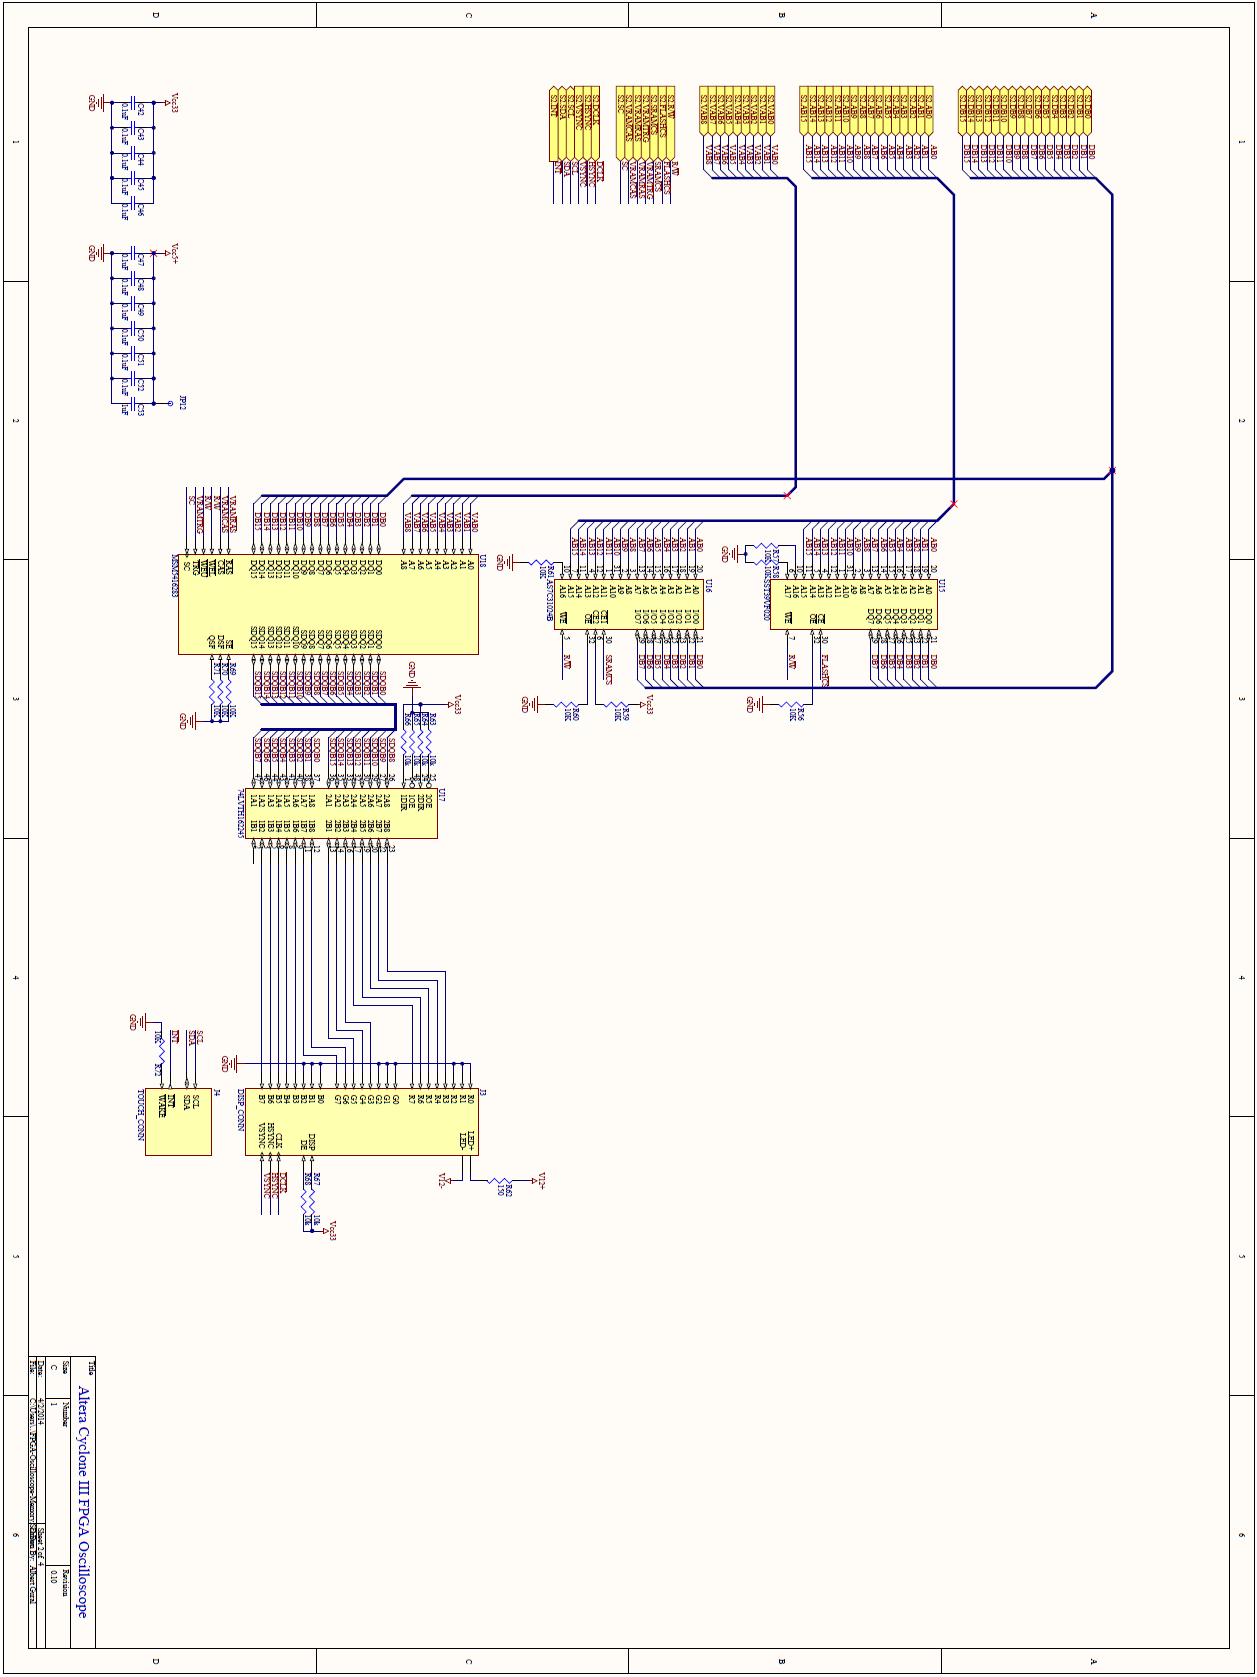
\includegraphics[width=6in]{circuit/memory_page.png}
		\caption{Memory schematic diagram}
\end{figure}

\begin{figure}[ht!]
    \centering
    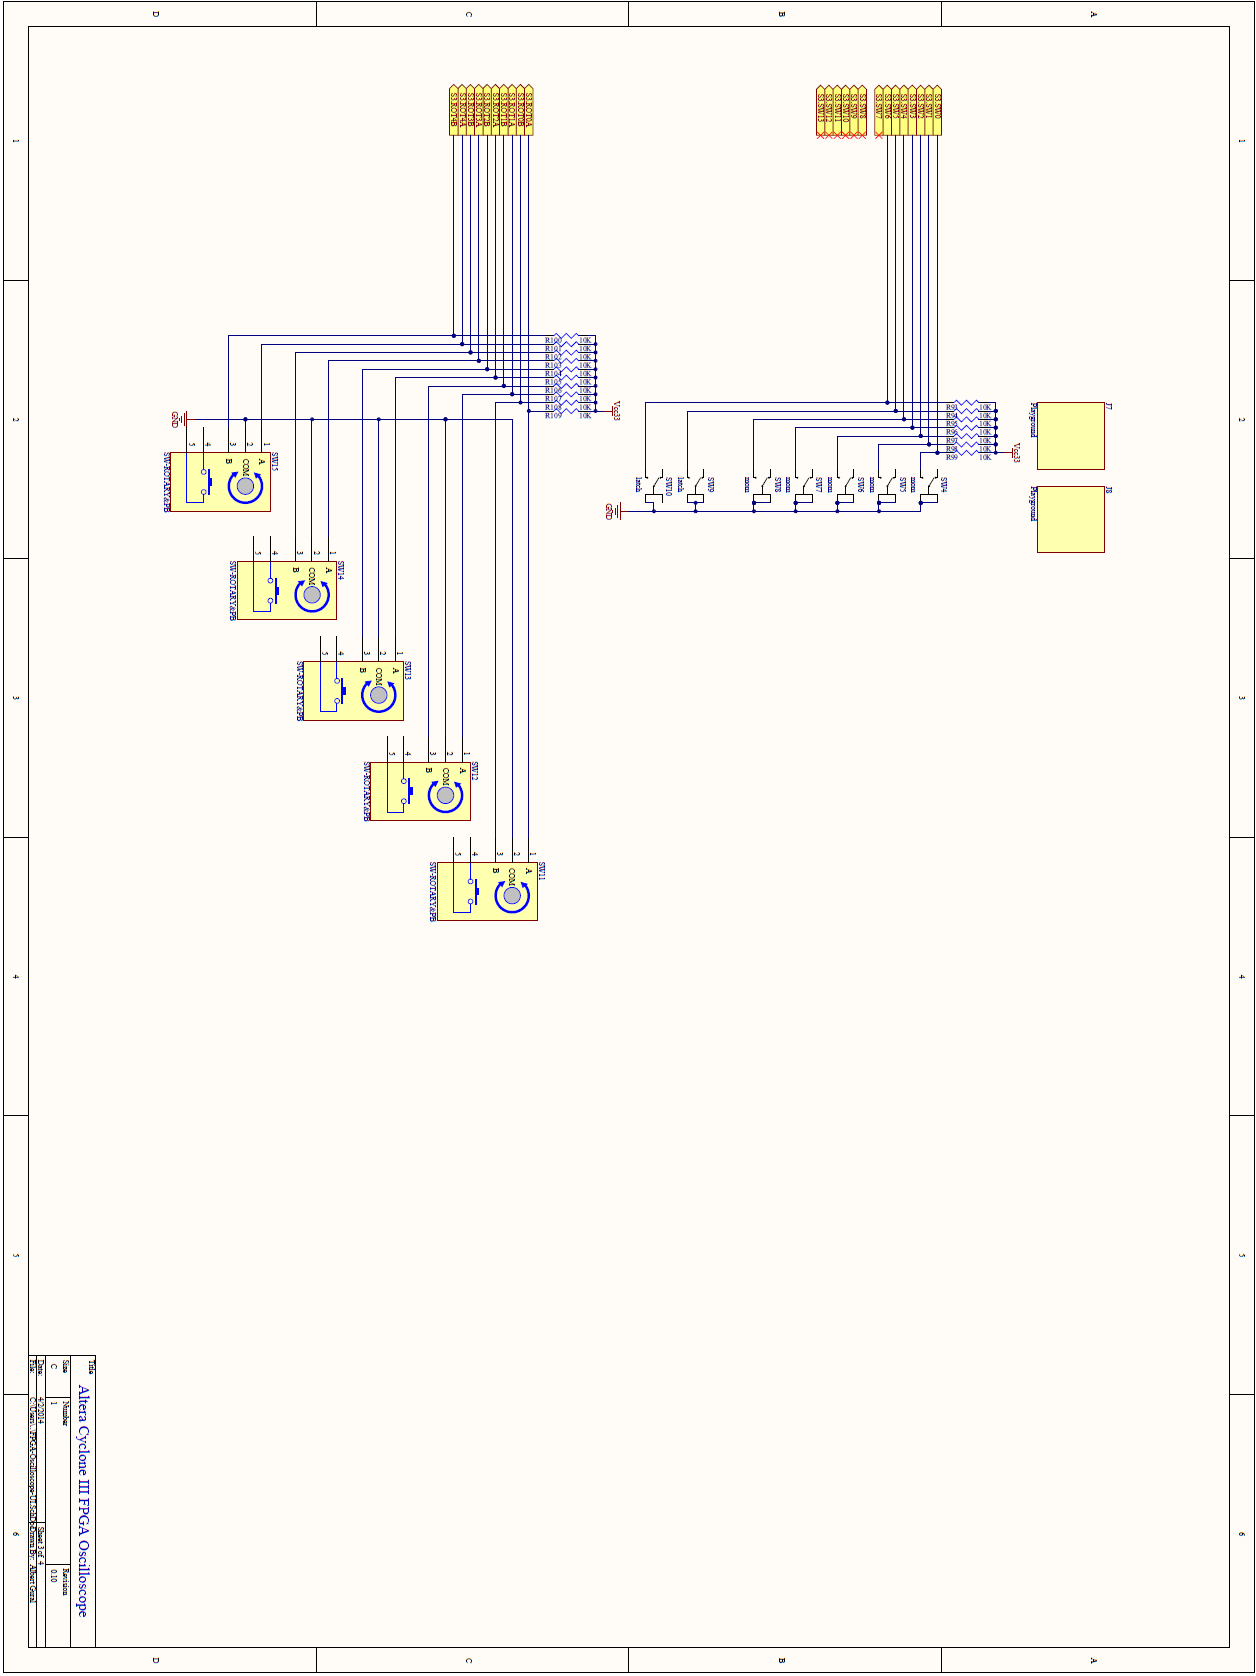
\includegraphics[width=6in]{circuit/switches_page.png}
		\caption{Switches schematic diagram}
\end{figure}

\chapter{Board Layouts} \label{App:boardlayouts}

\begin{figure}[ht!]
    \centering
    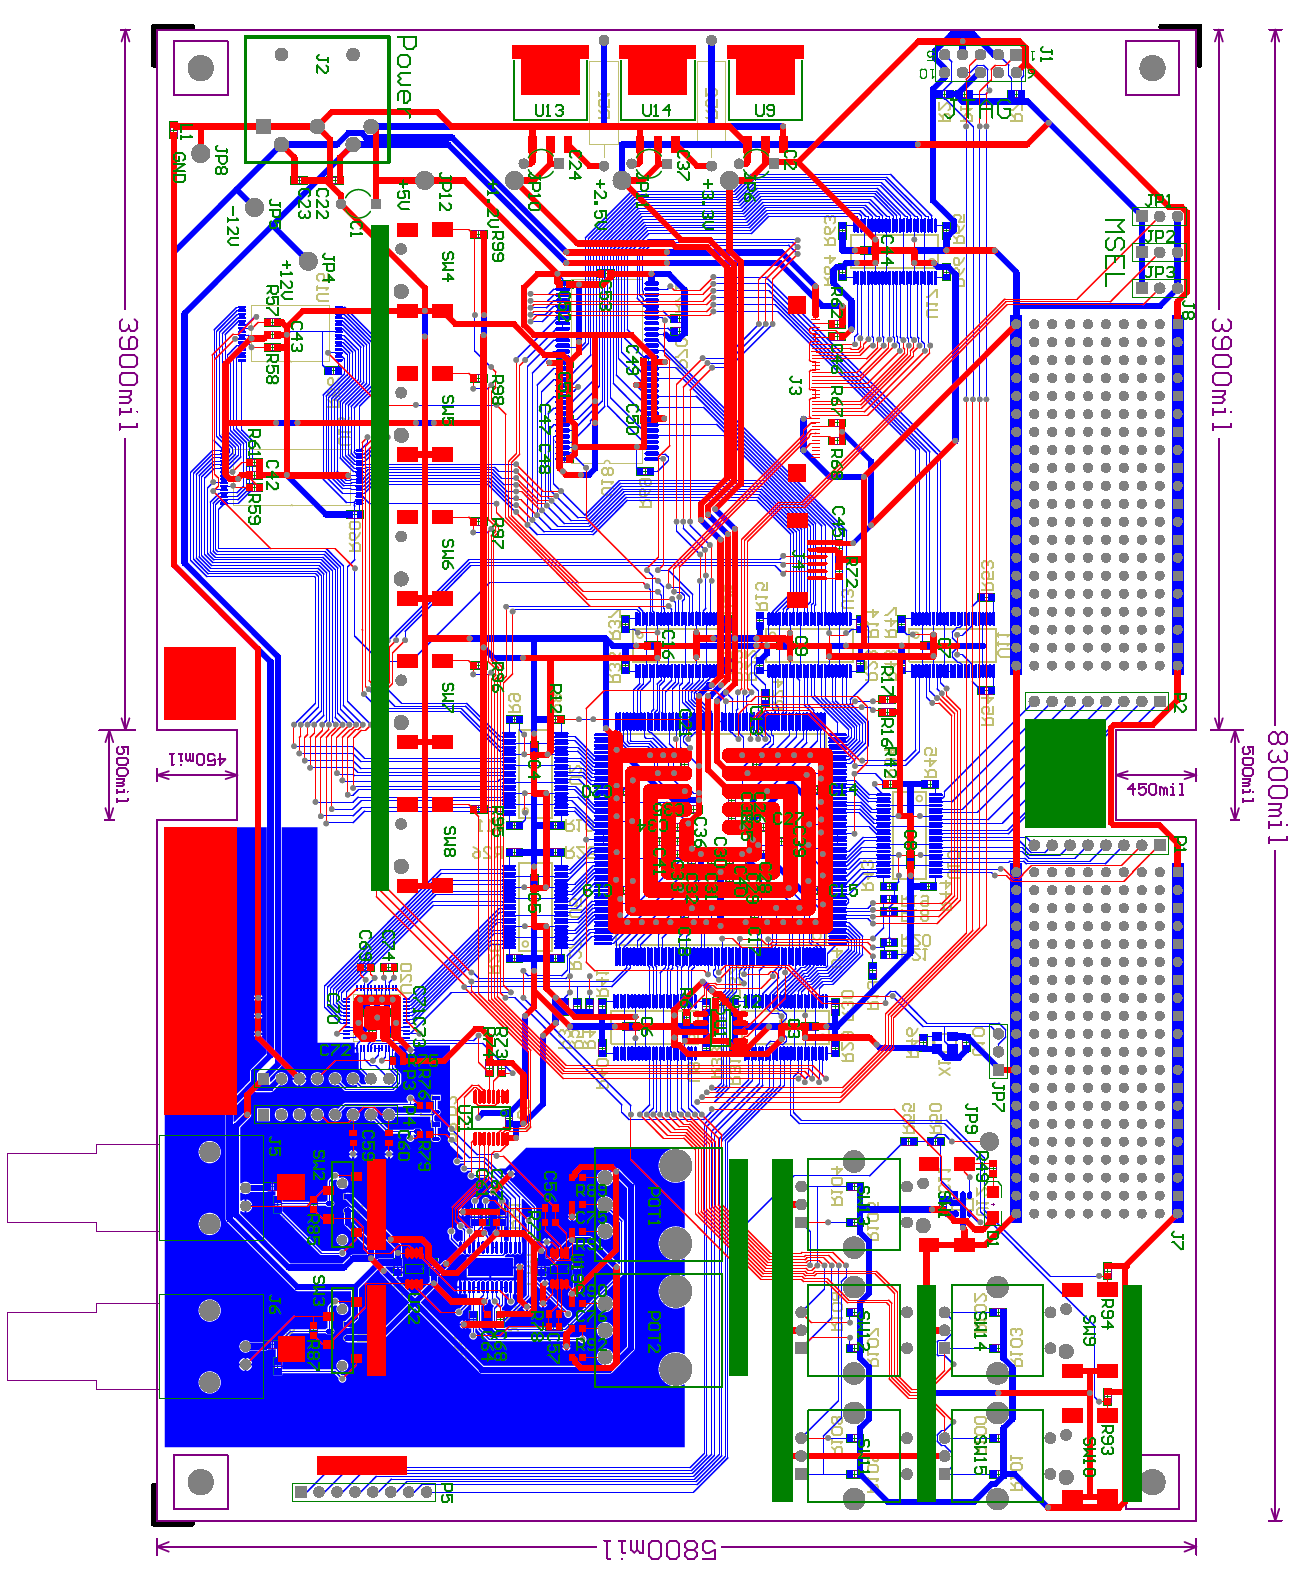
\includegraphics[width=6in]{circuit/board_page.png}
		\caption{Board layout (raw)}
\end{figure}

\chapter{FPGA Block Diagram Files} \label{App:fpgablockdiagrams}

\begin{figure}[ht!]
    \centering
    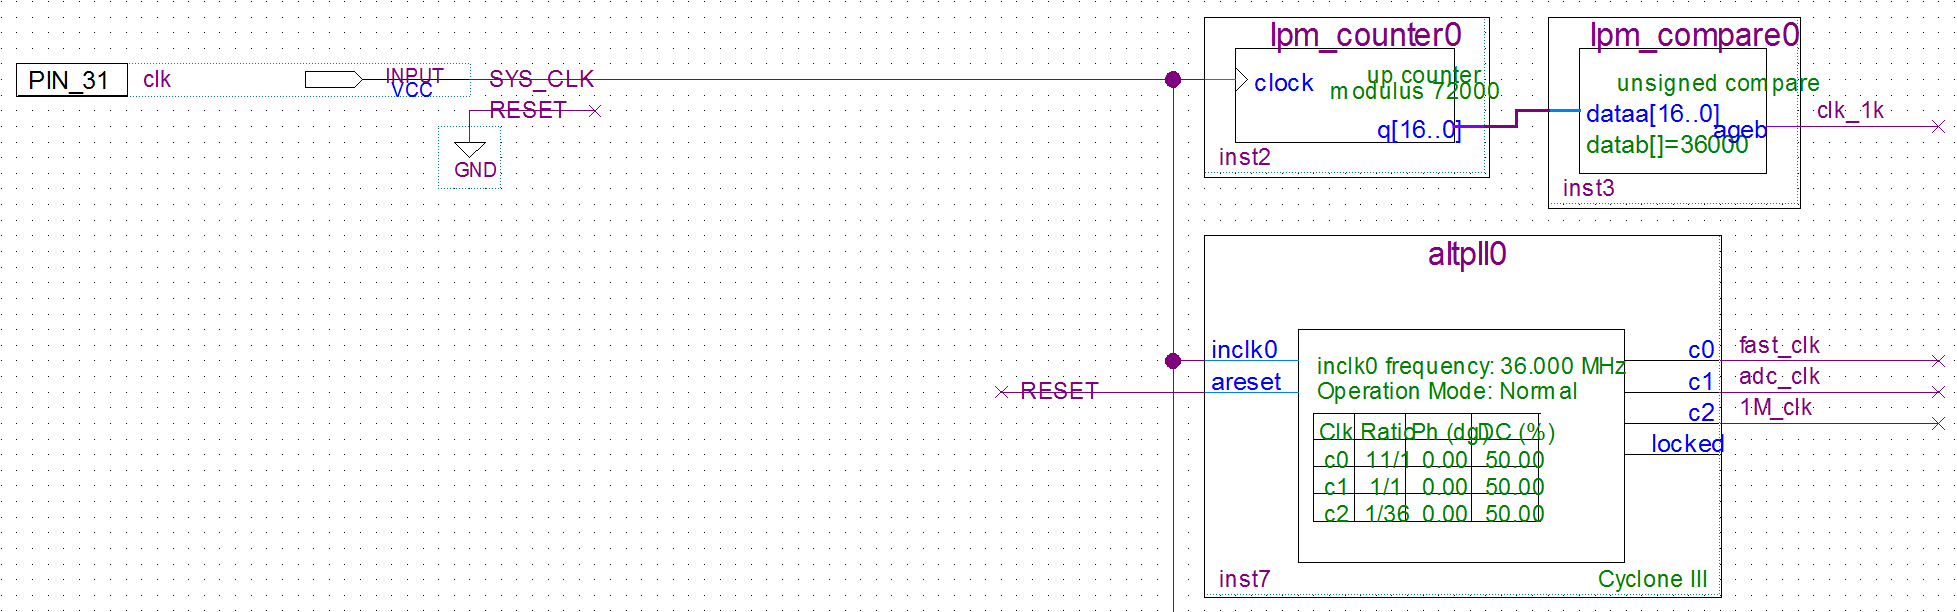
\includegraphics[width=6in]{fpga_logic/clocks.png}
		\caption{FPGA main clocks}
\end{figure}

\begin{figure}[ht!]
    \centering
    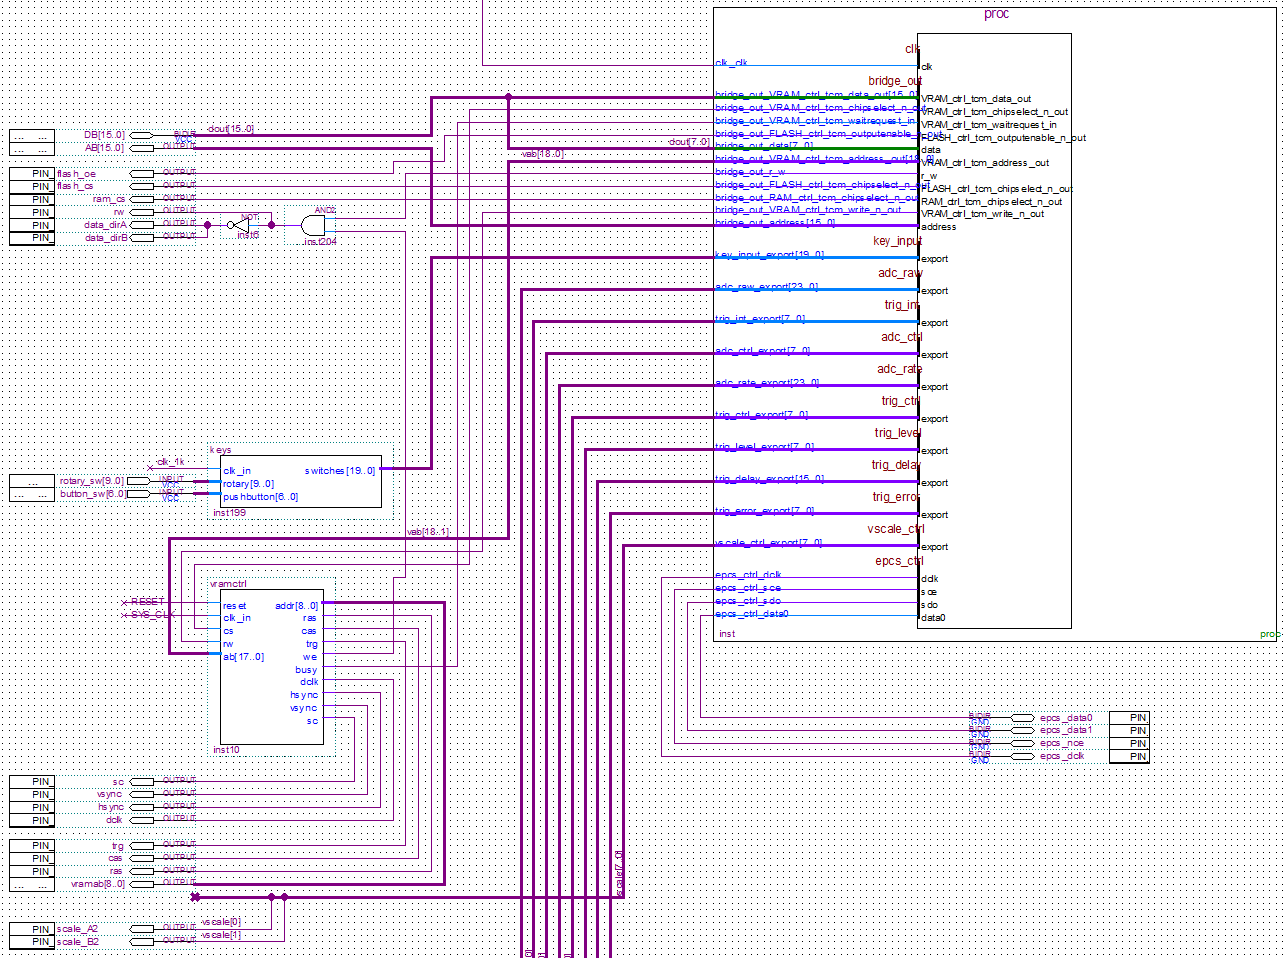
\includegraphics[width=6in]{fpga_logic/proc_overview.png}
		\caption{FPGA NIOS II processor block}
\end{figure}

\begin{figure}[ht!]
    \centering
    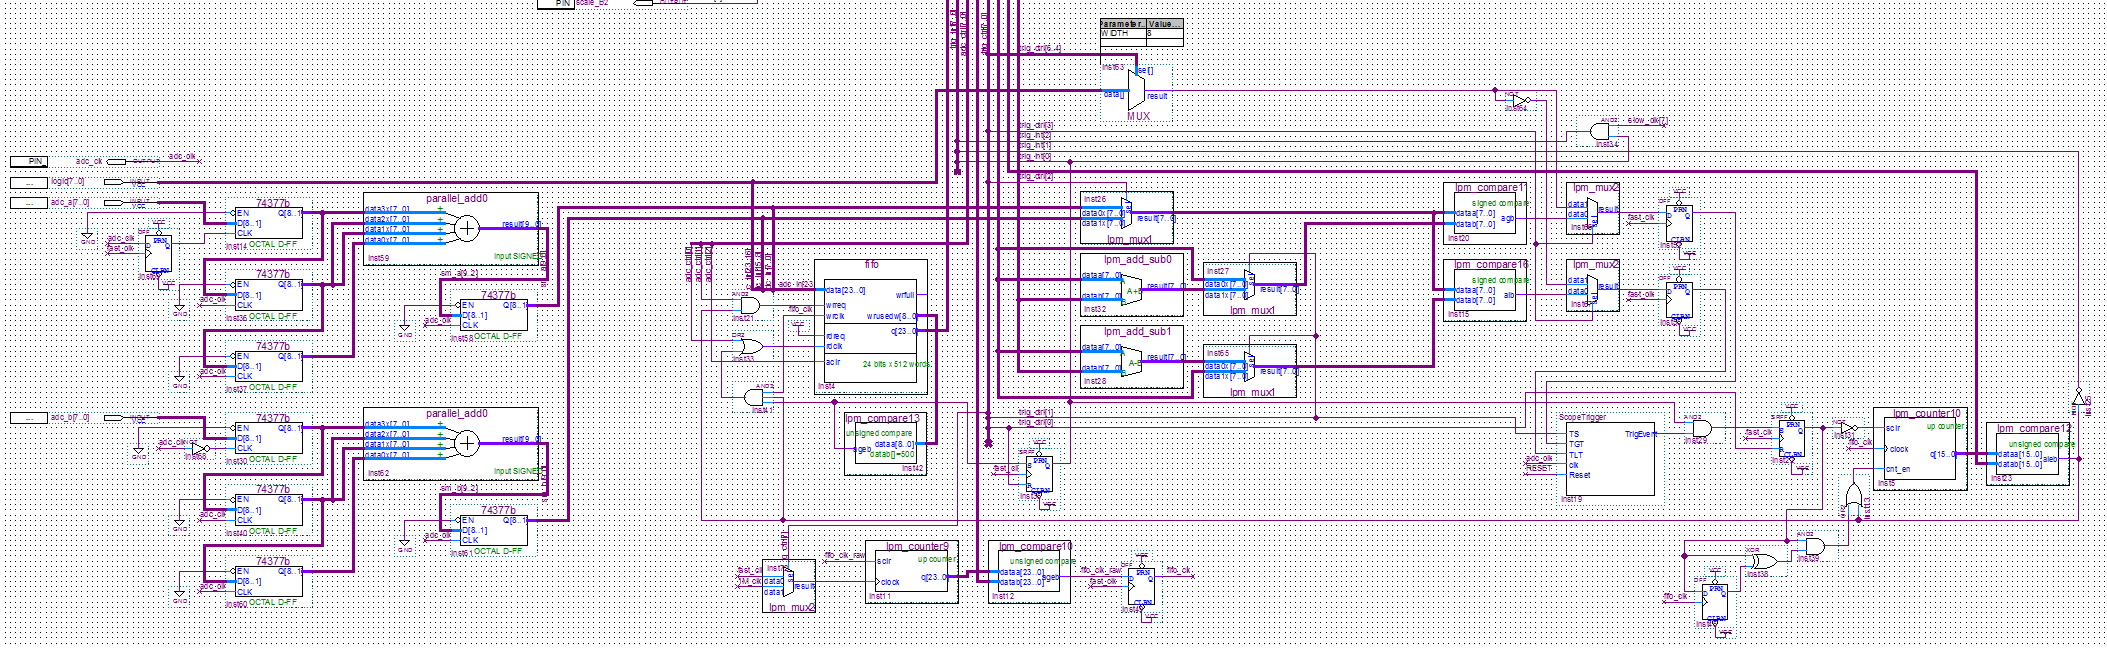
\includegraphics[width=6in]{fpga_logic/adc_overview.png}
		\caption{FPGA overview of scope sample handling}
\end{figure}

\begin{figure}[ht!]
    \centering
    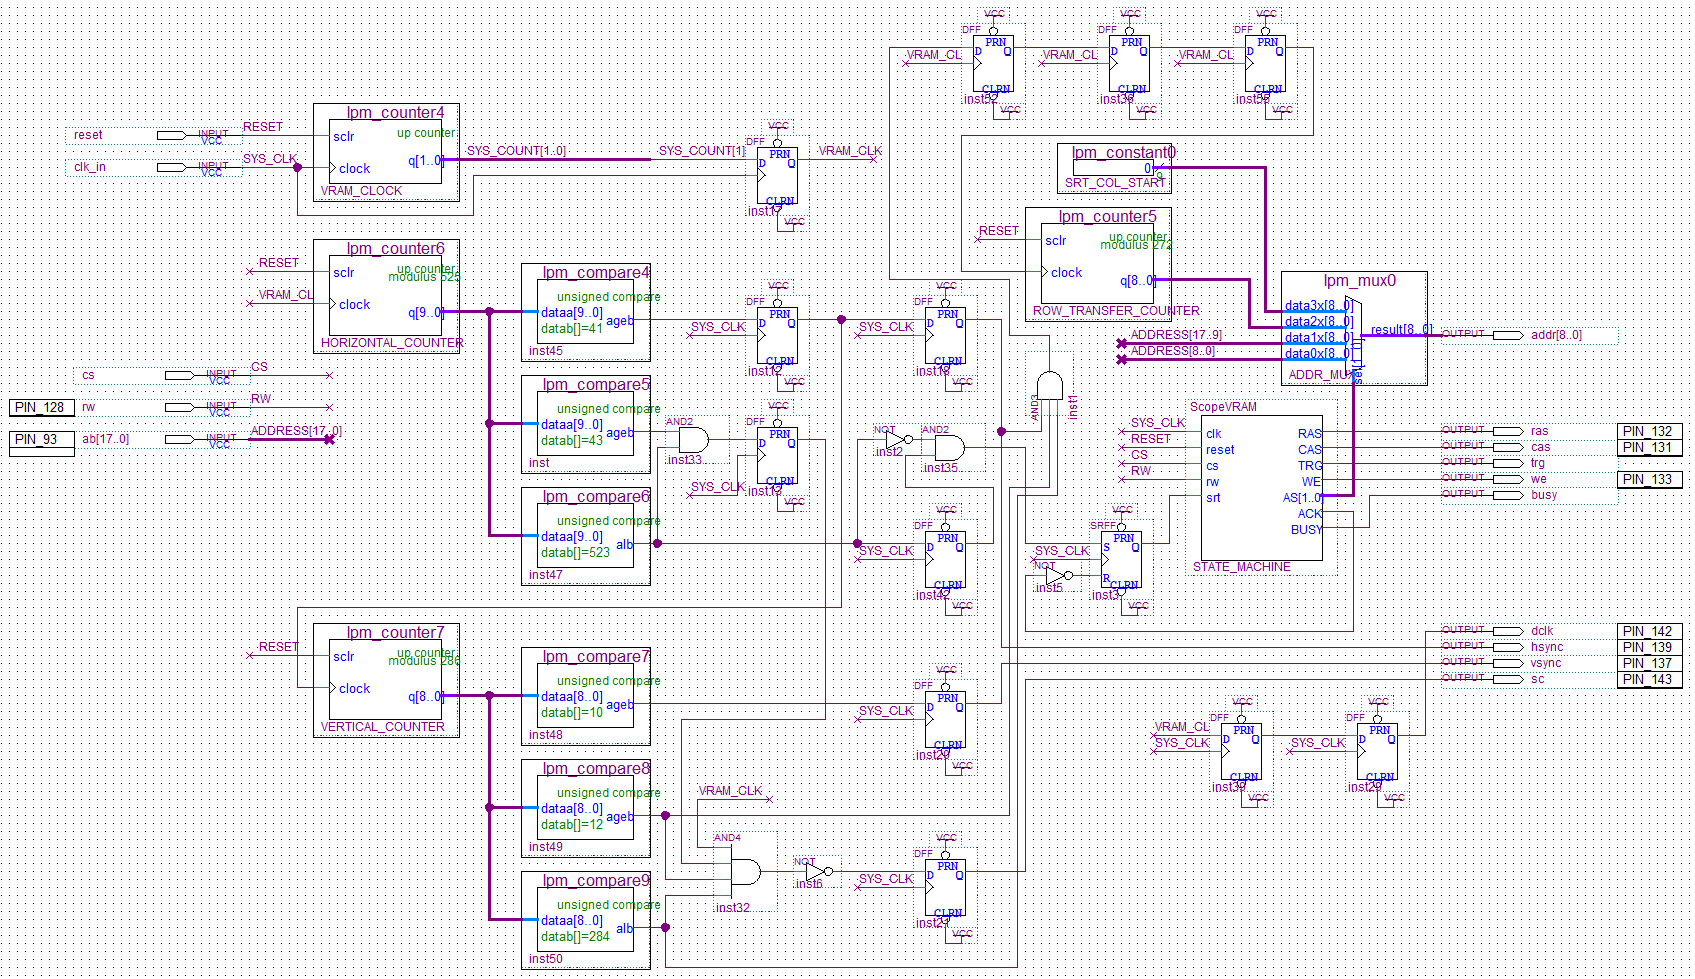
\includegraphics[width=6in]{fpga_logic/vram_disp_overview.png}
		\caption{FPGA overview of VRAM controller and display controller}
\end{figure}

\begin{figure}[ht!]
    \centering
    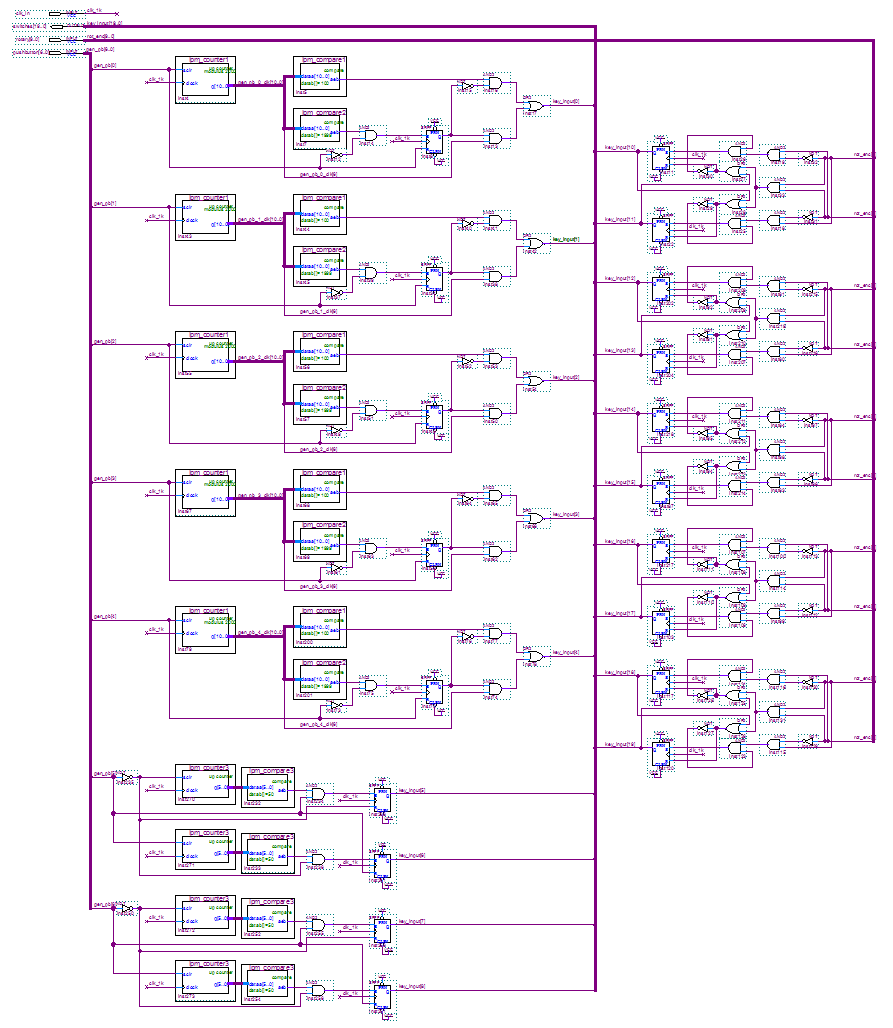
\includegraphics[width=6in]{fpga_logic/keys_overview.png}
		\caption{FPGA overview of key and rotary encoder input}
\end{figure}

\chapter{Memory Maps} \label{App:memorymaps}

\begin{figure}[ht!]
    \centering
    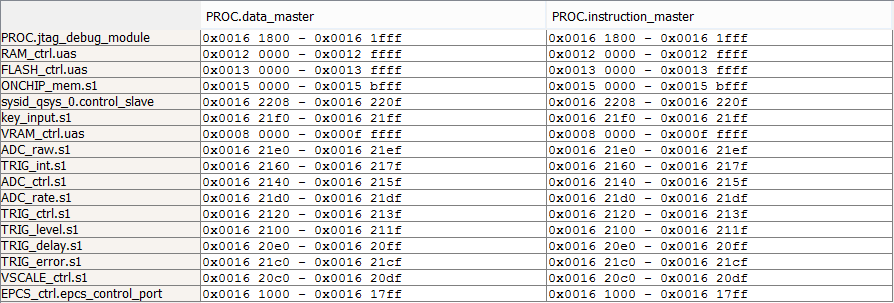
\includegraphics[width=6in]{fpga_logic/address_map.png}
		\caption{NIOS II address memory map}
\end{figure}

\chapter{Control Registers} \label{App:ctrlregs}

\begin{lstlisting}[language=C]
/*
 * system.h - SOPC Builder system and BSP software package information
 *
 * Machine generated for CPU 'PROC' in SOPC Builder design 'proc'
 * SOPC Builder design path: E:/agural/osc/proc.sopcinfo
 *
 * Generated: Sat Jun 14 01:48:11 GMT-08:00 2014
 */

/*
 * DO NOT MODIFY THIS FILE
 *
 * Changing this file will have subtle consequences
 * which will almost certainly lead to a nonfunctioning
 * system. If you do modify this file, be aware that your
 * changes will be overwritten and lost when this file
 * is generated again.
 *
 * DO NOT MODIFY THIS FILE
 */

/*
 * License Agreement
 *
 * Copyright (c) 2008
 * Altera Corporation, San Jose, California, USA.
 * All rights reserved.
 *
 * Permission is hereby granted, free of charge, to any person obtaining a
 * copy of this software and associated documentation files (the "Software"),
 * to deal in the Software without restriction, including without limitation
 * the rights to use, copy, modify, merge, publish, distribute, sublicense,
 * and/or sell copies of the Software, and to permit persons to whom the
 * Software is furnished to do so, subject to the following conditions:
 *
 * The above copyright notice and this permission notice shall be included in
 * all copies or substantial portions of the Software.
 *
 * THE SOFTWARE IS PROVIDED "AS IS", WITHOUT WARRANTY OF ANY KIND, EXPRESS OR
 * IMPLIED, INCLUDING BUT NOT LIMITED TO THE WARRANTIES OF MERCHANTABILITY,
 * FITNESS FOR A PARTICULAR PURPOSE AND NONINFRINGEMENT. IN NO EVENT SHALL THE
 * AUTHORS OR COPYRIGHT HOLDERS BE LIABLE FOR ANY CLAIM, DAMAGES OR OTHER
 * LIABILITY, WHETHER IN AN ACTION OF CONTRACT, TORT OR OTHERWISE, ARISING
 * FROM, OUT OF OR IN CONNECTION WITH THE SOFTWARE OR THE USE OR OTHER
 * DEALINGS IN THE SOFTWARE.
 *
 * This agreement shall be governed in all respects by the laws of the State
 * of California and by the laws of the United States of America.
 */

#ifndef __SYSTEM_H_
#define __SYSTEM_H_

/* Include definitions from linker script generator */
#include "linker.h"


/*
 * ADC_ctrl configuration
 *
 */

#define ADC_CTRL_BASE 0x162140
#define ADC_CTRL_BIT_CLEARING_EDGE_REGISTER 0
#define ADC_CTRL_BIT_MODIFYING_OUTPUT_REGISTER 1
#define ADC_CTRL_CAPTURE 0
#define ADC_CTRL_DATA_WIDTH 8
#define ADC_CTRL_DO_TEST_BENCH_WIRING 0
#define ADC_CTRL_DRIVEN_SIM_VALUE 0
#define ADC_CTRL_EDGE_TYPE "NONE"
#define ADC_CTRL_FREQ 36000000
#define ADC_CTRL_HAS_IN 0
#define ADC_CTRL_HAS_OUT 1
#define ADC_CTRL_HAS_TRI 0
#define ADC_CTRL_IRQ -1
#define ADC_CTRL_IRQ_INTERRUPT_CONTROLLER_ID -1
#define ADC_CTRL_IRQ_TYPE "NONE"
#define ADC_CTRL_NAME "/dev/ADC_ctrl"
#define ADC_CTRL_RESET_VALUE 0
#define ADC_CTRL_SPAN 32
#define ADC_CTRL_TYPE "altera_avalon_pio"
#define ALT_MODULE_CLASS_ADC_ctrl altera_avalon_pio


/*
 * ADC_rate configuration
 *
 */

#define ADC_RATE_BASE 0x1621d0
#define ADC_RATE_BIT_CLEARING_EDGE_REGISTER 0
#define ADC_RATE_BIT_MODIFYING_OUTPUT_REGISTER 0
#define ADC_RATE_CAPTURE 0
#define ADC_RATE_DATA_WIDTH 24
#define ADC_RATE_DO_TEST_BENCH_WIRING 0
#define ADC_RATE_DRIVEN_SIM_VALUE 0
#define ADC_RATE_EDGE_TYPE "NONE"
#define ADC_RATE_FREQ 36000000
#define ADC_RATE_HAS_IN 0
#define ADC_RATE_HAS_OUT 1
#define ADC_RATE_HAS_TRI 0
#define ADC_RATE_IRQ -1
#define ADC_RATE_IRQ_INTERRUPT_CONTROLLER_ID -1
#define ADC_RATE_IRQ_TYPE "NONE"
#define ADC_RATE_NAME "/dev/ADC_rate"
#define ADC_RATE_RESET_VALUE 0
#define ADC_RATE_SPAN 16
#define ADC_RATE_TYPE "altera_avalon_pio"
#define ALT_MODULE_CLASS_ADC_rate altera_avalon_pio


/*
 * ADC_raw configuration
 *
 */

#define ADC_RAW_BASE 0x1621e0
#define ADC_RAW_BIT_CLEARING_EDGE_REGISTER 0
#define ADC_RAW_BIT_MODIFYING_OUTPUT_REGISTER 0
#define ADC_RAW_CAPTURE 0
#define ADC_RAW_DATA_WIDTH 24
#define ADC_RAW_DO_TEST_BENCH_WIRING 0
#define ADC_RAW_DRIVEN_SIM_VALUE 0
#define ADC_RAW_EDGE_TYPE "NONE"
#define ADC_RAW_FREQ 36000000
#define ADC_RAW_HAS_IN 1
#define ADC_RAW_HAS_OUT 0
#define ADC_RAW_HAS_TRI 0
#define ADC_RAW_IRQ -1
#define ADC_RAW_IRQ_INTERRUPT_CONTROLLER_ID -1
#define ADC_RAW_IRQ_TYPE "NONE"
#define ADC_RAW_NAME "/dev/ADC_raw"
#define ADC_RAW_RESET_VALUE 0
#define ADC_RAW_SPAN 16
#define ADC_RAW_TYPE "altera_avalon_pio"
#define ALT_MODULE_CLASS_ADC_raw altera_avalon_pio


/*
 * CPU configuration
 *
 */

#define ALT_CPU_ARCHITECTURE "altera_nios2_qsys"
#define ALT_CPU_BIG_ENDIAN 0
#define ALT_CPU_BREAK_ADDR 0x00161820
#define ALT_CPU_CPU_FREQ 36000000u
#define ALT_CPU_CPU_ID_SIZE 1
#define ALT_CPU_CPU_ID_VALUE 0x00000000
#define ALT_CPU_CPU_IMPLEMENTATION "small"
#define ALT_CPU_DATA_ADDR_WIDTH 0x15
#define ALT_CPU_DCACHE_LINE_SIZE 0
#define ALT_CPU_DCACHE_LINE_SIZE_LOG2 0
#define ALT_CPU_DCACHE_SIZE 0
#define ALT_CPU_EXCEPTION_ADDR 0x00150020
#define ALT_CPU_FLUSHDA_SUPPORTED
#define ALT_CPU_FREQ 36000000
#define ALT_CPU_HARDWARE_DIVIDE_PRESENT 1
#define ALT_CPU_HARDWARE_MULTIPLY_PRESENT 1
#define ALT_CPU_HARDWARE_MULX_PRESENT 0
#define ALT_CPU_HAS_DEBUG_CORE 1
#define ALT_CPU_HAS_DEBUG_STUB
#define ALT_CPU_HAS_JMPI_INSTRUCTION
#define ALT_CPU_ICACHE_LINE_SIZE 32
#define ALT_CPU_ICACHE_LINE_SIZE_LOG2 5
#define ALT_CPU_ICACHE_SIZE 4096
#define ALT_CPU_INST_ADDR_WIDTH 0x15
#define ALT_CPU_NAME "PROC"
#define ALT_CPU_RESET_ADDR 0x00150000


/*
 * CPU configuration (with legacy prefix - don't use these anymore)
 *
 */

#define NIOS2_BIG_ENDIAN 0
#define NIOS2_BREAK_ADDR 0x00161820
#define NIOS2_CPU_FREQ 36000000u
#define NIOS2_CPU_ID_SIZE 1
#define NIOS2_CPU_ID_VALUE 0x00000000
#define NIOS2_CPU_IMPLEMENTATION "small"
#define NIOS2_DATA_ADDR_WIDTH 0x15
#define NIOS2_DCACHE_LINE_SIZE 0
#define NIOS2_DCACHE_LINE_SIZE_LOG2 0
#define NIOS2_DCACHE_SIZE 0
#define NIOS2_EXCEPTION_ADDR 0x00150020
#define NIOS2_FLUSHDA_SUPPORTED
#define NIOS2_HARDWARE_DIVIDE_PRESENT 1
#define NIOS2_HARDWARE_MULTIPLY_PRESENT 1
#define NIOS2_HARDWARE_MULX_PRESENT 0
#define NIOS2_HAS_DEBUG_CORE 1
#define NIOS2_HAS_DEBUG_STUB
#define NIOS2_HAS_JMPI_INSTRUCTION
#define NIOS2_ICACHE_LINE_SIZE 32
#define NIOS2_ICACHE_LINE_SIZE_LOG2 5
#define NIOS2_ICACHE_SIZE 4096
#define NIOS2_INST_ADDR_WIDTH 0x15
#define NIOS2_RESET_ADDR 0x00150000


/*
 * Define for each module class mastered by the CPU
 *
 */

#define __ALTERA_AVALON_EPCS_FLASH_CONTROLLER
#define __ALTERA_AVALON_ONCHIP_MEMORY2
#define __ALTERA_AVALON_PIO
#define __ALTERA_AVALON_SYSID_QSYS
#define __ALTERA_GENERIC_TRISTATE_CONTROLLER
#define __ALTERA_NIOS2_QSYS


/*
 * EPCS_ctrl configuration
 *
 */

#define ALT_MODULE_CLASS_EPCS_ctrl altera_avalon_epcs_flash_controller
#define EPCS_CTRL_BASE 0x161000
#define EPCS_CTRL_IRQ -1
#define EPCS_CTRL_IRQ_INTERRUPT_CONTROLLER_ID -1
#define EPCS_CTRL_NAME "/dev/EPCS_ctrl"
#define EPCS_CTRL_REGISTER_OFFSET 1024
#define EPCS_CTRL_SPAN 2048
#define EPCS_CTRL_TYPE "altera_avalon_epcs_flash_controller"


/*
 * FLASH_ctrl configuration
 *
 */

#define ALT_MODULE_CLASS_FLASH_ctrl altera_generic_tristate_controller
#define FLASH_CTRL_BASE 0x130000
#define FLASH_CTRL_IRQ -1
#define FLASH_CTRL_IRQ_INTERRUPT_CONTROLLER_ID -1
#define FLASH_CTRL_NAME "/dev/FLASH_ctrl"
#define FLASH_CTRL_SIZE 65536
#define FLASH_CTRL_SPAN 65536
#define FLASH_CTRL_TYPE "altera_generic_tristate_controller"


/*
 * ONCHIP_mem configuration
 *
 */

#define ALT_MODULE_CLASS_ONCHIP_mem altera_avalon_onchip_memory2
#define ONCHIP_MEM_ALLOW_IN_SYSTEM_MEMORY_CONTENT_EDITOR 0
#define ONCHIP_MEM_ALLOW_MRAM_SIM_CONTENTS_ONLY_FILE 0
#define ONCHIP_MEM_BASE 0x150000
#define ONCHIP_MEM_CONTENTS_INFO ""
#define ONCHIP_MEM_DUAL_PORT 0
#define ONCHIP_MEM_GUI_RAM_BLOCK_TYPE "AUTO"
#define ONCHIP_MEM_INIT_CONTENTS_FILE "proc_ONCHIP_mem"
#define ONCHIP_MEM_INIT_MEM_CONTENT 1
#define ONCHIP_MEM_INSTANCE_ID "NONE"
#define ONCHIP_MEM_IRQ -1
#define ONCHIP_MEM_IRQ_INTERRUPT_CONTROLLER_ID -1
#define ONCHIP_MEM_NAME "/dev/ONCHIP_mem"
#define ONCHIP_MEM_NON_DEFAULT_INIT_FILE_ENABLED 0
#define ONCHIP_MEM_RAM_BLOCK_TYPE "AUTO"
#define ONCHIP_MEM_READ_DURING_WRITE_MODE "DONT_CARE"
#define ONCHIP_MEM_SINGLE_CLOCK_OP 0
#define ONCHIP_MEM_SIZE_MULTIPLE 1
#define ONCHIP_MEM_SIZE_VALUE 49152
#define ONCHIP_MEM_SPAN 49152
#define ONCHIP_MEM_TYPE "altera_avalon_onchip_memory2"
#define ONCHIP_MEM_WRITABLE 1


/*
 * RAM_ctrl configuration
 *
 */

#define ALT_MODULE_CLASS_RAM_ctrl altera_generic_tristate_controller
#define RAM_CTRL_BASE 0x120000
#define RAM_CTRL_IRQ -1
#define RAM_CTRL_IRQ_INTERRUPT_CONTROLLER_ID -1
#define RAM_CTRL_NAME "/dev/RAM_ctrl"
#define RAM_CTRL_SIZE 65536
#define RAM_CTRL_SPAN 65536
#define RAM_CTRL_TYPE "altera_generic_tristate_controller"


/*
 * System configuration
 *
 */

#define ALT_DEVICE_FAMILY "Cyclone III"
#define ALT_ENHANCED_INTERRUPT_API_PRESENT
#define ALT_IRQ_BASE NULL
#define ALT_LOG_PORT "/dev/null"
#define ALT_LOG_PORT_BASE 0x0
#define ALT_LOG_PORT_DEV null
#define ALT_LOG_PORT_TYPE ""
#define ALT_NUM_EXTERNAL_INTERRUPT_CONTROLLERS 0
#define ALT_NUM_INTERNAL_INTERRUPT_CONTROLLERS 1
#define ALT_NUM_INTERRUPT_CONTROLLERS 1
#define ALT_STDERR "/dev/null"
#define ALT_STDERR_BASE 0x0
#define ALT_STDERR_DEV null
#define ALT_STDERR_TYPE ""
#define ALT_STDIN "/dev/null"
#define ALT_STDIN_BASE 0x0
#define ALT_STDIN_DEV null
#define ALT_STDIN_TYPE ""
#define ALT_STDOUT "/dev/null"
#define ALT_STDOUT_BASE 0x0
#define ALT_STDOUT_DEV null
#define ALT_STDOUT_TYPE ""
#define ALT_SYSTEM_NAME "proc"


/*
 * TRIG_ctrl configuration
 *
 */

#define ALT_MODULE_CLASS_TRIG_ctrl altera_avalon_pio
#define TRIG_CTRL_BASE 0x162120
#define TRIG_CTRL_BIT_CLEARING_EDGE_REGISTER 0
#define TRIG_CTRL_BIT_MODIFYING_OUTPUT_REGISTER 1
#define TRIG_CTRL_CAPTURE 0
#define TRIG_CTRL_DATA_WIDTH 8
#define TRIG_CTRL_DO_TEST_BENCH_WIRING 0
#define TRIG_CTRL_DRIVEN_SIM_VALUE 0
#define TRIG_CTRL_EDGE_TYPE "NONE"
#define TRIG_CTRL_FREQ 36000000
#define TRIG_CTRL_HAS_IN 0
#define TRIG_CTRL_HAS_OUT 1
#define TRIG_CTRL_HAS_TRI 0
#define TRIG_CTRL_IRQ -1
#define TRIG_CTRL_IRQ_INTERRUPT_CONTROLLER_ID -1
#define TRIG_CTRL_IRQ_TYPE "NONE"
#define TRIG_CTRL_NAME "/dev/TRIG_ctrl"
#define TRIG_CTRL_RESET_VALUE 0
#define TRIG_CTRL_SPAN 32
#define TRIG_CTRL_TYPE "altera_avalon_pio"


/*
 * TRIG_delay configuration
 *
 */

#define ALT_MODULE_CLASS_TRIG_delay altera_avalon_pio
#define TRIG_DELAY_BASE 0x1620e0
#define TRIG_DELAY_BIT_CLEARING_EDGE_REGISTER 0
#define TRIG_DELAY_BIT_MODIFYING_OUTPUT_REGISTER 1
#define TRIG_DELAY_CAPTURE 0
#define TRIG_DELAY_DATA_WIDTH 16
#define TRIG_DELAY_DO_TEST_BENCH_WIRING 0
#define TRIG_DELAY_DRIVEN_SIM_VALUE 0
#define TRIG_DELAY_EDGE_TYPE "NONE"
#define TRIG_DELAY_FREQ 36000000
#define TRIG_DELAY_HAS_IN 0
#define TRIG_DELAY_HAS_OUT 1
#define TRIG_DELAY_HAS_TRI 0
#define TRIG_DELAY_IRQ -1
#define TRIG_DELAY_IRQ_INTERRUPT_CONTROLLER_ID -1
#define TRIG_DELAY_IRQ_TYPE "NONE"
#define TRIG_DELAY_NAME "/dev/TRIG_delay"
#define TRIG_DELAY_RESET_VALUE 0
#define TRIG_DELAY_SPAN 32
#define TRIG_DELAY_TYPE "altera_avalon_pio"


/*
 * TRIG_error configuration
 *
 */

#define ALT_MODULE_CLASS_TRIG_error altera_avalon_pio
#define TRIG_ERROR_BASE 0x1621c0
#define TRIG_ERROR_BIT_CLEARING_EDGE_REGISTER 0
#define TRIG_ERROR_BIT_MODIFYING_OUTPUT_REGISTER 0
#define TRIG_ERROR_CAPTURE 0
#define TRIG_ERROR_DATA_WIDTH 8
#define TRIG_ERROR_DO_TEST_BENCH_WIRING 0
#define TRIG_ERROR_DRIVEN_SIM_VALUE 0
#define TRIG_ERROR_EDGE_TYPE "NONE"
#define TRIG_ERROR_FREQ 36000000
#define TRIG_ERROR_HAS_IN 0
#define TRIG_ERROR_HAS_OUT 1
#define TRIG_ERROR_HAS_TRI 0
#define TRIG_ERROR_IRQ -1
#define TRIG_ERROR_IRQ_INTERRUPT_CONTROLLER_ID -1
#define TRIG_ERROR_IRQ_TYPE "NONE"
#define TRIG_ERROR_NAME "/dev/TRIG_error"
#define TRIG_ERROR_RESET_VALUE 0
#define TRIG_ERROR_SPAN 16
#define TRIG_ERROR_TYPE "altera_avalon_pio"


/*
 * TRIG_int configuration
 *
 */

#define ALT_MODULE_CLASS_TRIG_int altera_avalon_pio
#define TRIG_INT_BASE 0x162160
#define TRIG_INT_BIT_CLEARING_EDGE_REGISTER 1
#define TRIG_INT_BIT_MODIFYING_OUTPUT_REGISTER 1
#define TRIG_INT_CAPTURE 1
#define TRIG_INT_DATA_WIDTH 8
#define TRIG_INT_DO_TEST_BENCH_WIRING 0
#define TRIG_INT_DRIVEN_SIM_VALUE 0
#define TRIG_INT_EDGE_TYPE "RISING"
#define TRIG_INT_FREQ 36000000
#define TRIG_INT_HAS_IN 1
#define TRIG_INT_HAS_OUT 0
#define TRIG_INT_HAS_TRI 0
#define TRIG_INT_IRQ 6
#define TRIG_INT_IRQ_INTERRUPT_CONTROLLER_ID 0
#define TRIG_INT_IRQ_TYPE "EDGE"
#define TRIG_INT_NAME "/dev/TRIG_int"
#define TRIG_INT_RESET_VALUE 0
#define TRIG_INT_SPAN 32
#define TRIG_INT_TYPE "altera_avalon_pio"


/*
 * TRIG_level configuration
 *
 */

#define ALT_MODULE_CLASS_TRIG_level altera_avalon_pio
#define TRIG_LEVEL_BASE 0x162100
#define TRIG_LEVEL_BIT_CLEARING_EDGE_REGISTER 0
#define TRIG_LEVEL_BIT_MODIFYING_OUTPUT_REGISTER 1
#define TRIG_LEVEL_CAPTURE 0
#define TRIG_LEVEL_DATA_WIDTH 8
#define TRIG_LEVEL_DO_TEST_BENCH_WIRING 0
#define TRIG_LEVEL_DRIVEN_SIM_VALUE 0
#define TRIG_LEVEL_EDGE_TYPE "NONE"
#define TRIG_LEVEL_FREQ 36000000
#define TRIG_LEVEL_HAS_IN 0
#define TRIG_LEVEL_HAS_OUT 1
#define TRIG_LEVEL_HAS_TRI 0
#define TRIG_LEVEL_IRQ -1
#define TRIG_LEVEL_IRQ_INTERRUPT_CONTROLLER_ID -1
#define TRIG_LEVEL_IRQ_TYPE "NONE"
#define TRIG_LEVEL_NAME "/dev/TRIG_level"
#define TRIG_LEVEL_RESET_VALUE 0
#define TRIG_LEVEL_SPAN 32
#define TRIG_LEVEL_TYPE "altera_avalon_pio"


/*
 * VRAM_ctrl configuration
 *
 */

#define ALT_MODULE_CLASS_VRAM_ctrl altera_generic_tristate_controller
#define VRAM_CTRL_BASE 0x80000
#define VRAM_CTRL_IRQ -1
#define VRAM_CTRL_IRQ_INTERRUPT_CONTROLLER_ID -1
#define VRAM_CTRL_NAME "/dev/VRAM_ctrl"
#define VRAM_CTRL_SPAN 524288
#define VRAM_CTRL_TYPE "altera_generic_tristate_controller"


/*
 * VSCALE_ctrl configuration
 *
 */

#define ALT_MODULE_CLASS_VSCALE_ctrl altera_avalon_pio
#define VSCALE_CTRL_BASE 0x1620c0
#define VSCALE_CTRL_BIT_CLEARING_EDGE_REGISTER 0
#define VSCALE_CTRL_BIT_MODIFYING_OUTPUT_REGISTER 1
#define VSCALE_CTRL_CAPTURE 0
#define VSCALE_CTRL_DATA_WIDTH 8
#define VSCALE_CTRL_DO_TEST_BENCH_WIRING 0
#define VSCALE_CTRL_DRIVEN_SIM_VALUE 0
#define VSCALE_CTRL_EDGE_TYPE "NONE"
#define VSCALE_CTRL_FREQ 36000000
#define VSCALE_CTRL_HAS_IN 0
#define VSCALE_CTRL_HAS_OUT 1
#define VSCALE_CTRL_HAS_TRI 0
#define VSCALE_CTRL_IRQ -1
#define VSCALE_CTRL_IRQ_INTERRUPT_CONTROLLER_ID -1
#define VSCALE_CTRL_IRQ_TYPE "NONE"
#define VSCALE_CTRL_NAME "/dev/VSCALE_ctrl"
#define VSCALE_CTRL_RESET_VALUE 0
#define VSCALE_CTRL_SPAN 32
#define VSCALE_CTRL_TYPE "altera_avalon_pio"


/*
 * hal configuration
 *
 */

#define ALT_MAX_FD 32
#define ALT_SYS_CLK none
#define ALT_TIMESTAMP_CLK none


/*
 * key_input configuration
 *
 */

#define ALT_MODULE_CLASS_key_input altera_avalon_pio
#define KEY_INPUT_BASE 0x1621f0
#define KEY_INPUT_BIT_CLEARING_EDGE_REGISTER 1
#define KEY_INPUT_BIT_MODIFYING_OUTPUT_REGISTER 0
#define KEY_INPUT_CAPTURE 1
#define KEY_INPUT_DATA_WIDTH 20
#define KEY_INPUT_DO_TEST_BENCH_WIRING 0
#define KEY_INPUT_DRIVEN_SIM_VALUE 0
#define KEY_INPUT_EDGE_TYPE "RISING"
#define KEY_INPUT_FREQ 36000000
#define KEY_INPUT_HAS_IN 1
#define KEY_INPUT_HAS_OUT 0
#define KEY_INPUT_HAS_TRI 0
#define KEY_INPUT_IRQ 5
#define KEY_INPUT_IRQ_INTERRUPT_CONTROLLER_ID 0
#define KEY_INPUT_IRQ_TYPE "EDGE"
#define KEY_INPUT_NAME "/dev/key_input"
#define KEY_INPUT_RESET_VALUE 0
#define KEY_INPUT_SPAN 16
#define KEY_INPUT_TYPE "altera_avalon_pio"


/*
 * sysid_qsys_0 configuration
 *
 */

#define ALT_MODULE_CLASS_sysid_qsys_0 altera_avalon_sysid_qsys
#define SYSID_QSYS_0_BASE 0x162208
#define SYSID_QSYS_0_ID -1431655766
#define SYSID_QSYS_0_IRQ -1
#define SYSID_QSYS_0_IRQ_INTERRUPT_CONTROLLER_ID -1
#define SYSID_QSYS_0_NAME "/dev/sysid_qsys_0"
#define SYSID_QSYS_0_SPAN 8
#define SYSID_QSYS_0_TIMESTAMP 1402739081
#define SYSID_QSYS_0_TYPE "altera_avalon_sysid_qsys"

#endif /* __SYSTEM_H_ */
\end{lstlisting}

\chapter{VHDL Code} \label{App:vhdlcode}

\section{VRAM State Machine Code}
\begin{lstlisting}[language=vhdl]
----------------------------------------------------------------------------
--
--  Oscilloscope VRAM State Machine
--
--  This is an implementation of a VRAM State machine for a digital scope in
--  VHDL.  There are three inputs to the system, one selects the trigger
--  slope and the other two determine the relationship between the trigger
--  level and the signal level.  The only output is a trigger signal which
--  indicates a trigger event has occurred.
--
--  The file contains multiple architectures for a Moore state machine
--  implementation to demonstrate the different ways of building a state
--  machine.
--
--
--  Revision History:
--     2014/02/23 Albert Gural      Created file and updated with VRAM
--                                  state machine.
--		 2014/06/07 Albert Gural		Added idle states to improve r/w speeds.
--
----------------------------------------------------------------------------


-- bring in the necessary packages
library  ieee;
use  ieee.std_logic_1164.all;


--
--  Oscilloscope VRAM entity declaration
--

entity  ScopeVRAM  is
    port (
        clk        :  in  std_logic;      -- clock input
        reset      :  in  std_logic;      -- reset to idle state (active low)
        cs         :  in  std_logic;      -- whether CPU is requesting R/W (active low)
        rw         :  in  std_logic;      -- whether CPU is requesting R or W
        srt        :  in  std_logic;      -- display requesting serial row transfer
        RAS        :  out std_logic;      -- row address select output
        CAS        :  out std_logic;      -- col address select output
        TRG        :  out std_logic;      -- trigger output (active low)
        WE         :  out std_logic;      -- write enable output (active low)
        AS         :  out std_logic_vector(1 downto 0); -- address select
                                                        -- 00 = low 9 bits
                                                        -- 01 = high 9 bits
                                                        -- 10 = row transfer
                                                        -- 11 = col transfer (0)
        ACK        :  out std_logic;      -- send acknowledge back to display driver
        BUSY       :  out std_logic       -- busy signal to CPU for read/write
    );
end  ScopeVRAM;

--
--  Oscilloscope VRAM Moore State Machine
--     State Assignment Architecture
--
--  This architecture just shows the basic state machine syntax when the state
--  assignments are made manually.  This is useful for minimizing output
--  decoding logic and avoiding glitches in the output (due to the decoding
--  logic).
--

architecture  assign_statebits  of  ScopeVRAM  is

    subtype  states  is  std_logic_vector(12 downto 0);     -- state type

    -- define the actual states as constants
    -- bits: [RAS][CAS][TRG][WE][AS<2>][ACK][BUSY]
    --       [type <000 IDLE, 010 READ, 011 WRITE, 100 REFRESH, 101 TRANSFER>]
    --       [number <00, 01, ...>]
    constant  IDLE      : states := "1111011100000";  -- idle (can accept R/W)
    constant  IDLE2     : states := "1111011100001";  -- idle (can accept R/W)
    constant  IDLE3     : states := "1111011100010";  -- idle (can accept R/W)
    constant  IDLE4     : states := "1111011100011";  -- idle (can accept R/W, srt, refresh)
    constant  READ1     : states := "1111011101000";  -- read cycle
    constant  READ2     : states := "0111011101000";  -- read cycle
    constant  READ3     : states := "0101001101000";  -- read cycle
    constant  READ4     : states := "0001001101000";  -- read cycle
    constant  READ5     : states := "0001001101001";  -- read cycle
    constant  READ6     : states := "0001001001010";  -- read cycle
    constant  READ7     : states := "1111001101000";  -- read cycle
    constant  READ8     : states := "1111001101001";  -- read cycle
    constant  READ9     : states := "1111001101010";  -- read cycle
    constant  WRITE1    : states := "0111011101100";  -- write cycle
    constant  WRITE2    : states := "0110001101100";  -- write cycle
    constant  WRITE3    : states := "0010001101100";  -- write cycle
    constant  WRITE4    : states := "0010001001101";  -- write cycle
    constant  WRITE5    : states := "1111001101100";  -- write cycle
    constant  WRITE6    : states := "1111001101101";  -- write cycle
    constant  WRITE7    : states := "1111001101110";  -- write cycle
    constant  TRANSFER1 : states := "1101101110100";  -- transfer cycle
    constant  TRANSFER2 : states := "0101101110100";  -- transfer cycle
    constant  TRANSFER3 : states := "0111111110100";  -- transfer cycle
    constant  TRANSFER4 : states := "0011111110100";  -- transfer cycle
    constant  TRANSFER5 : states := "1111010110100";  -- transfer cycle
    constant  TRANSFER6 : states := "1111011110100";  -- transfer cycle
    constant  REFRESH1  : states := "1111001110000";  -- refresh cycle
    constant  REFRESH2  : states := "1111001110001";  -- refresh cycle
    constant  REFRESH3  : states := "1011001110000";  -- refresh cycle
    constant  REFRESH4  : states := "0011001110000";  -- refresh cycle
    constant  REFRESH5  : states := "0011001110001";  -- refresh cycle
    constant  REFRESH6  : states := "0011001110010";  -- refresh cycle
    constant  REFRESH7  : states := "1111001110010";  -- refresh cycle
    constant  REFRESH8  : states := "1111001110011";  -- refresh cycle


    signal  CurrentState  :  states;    -- current state
    signal  NextState     :  states;    -- next state

begin


    -- the output is always the high bit of the state encoding
    RAS  <= CurrentState(12);
    CAS  <= CurrentState(11);
    TRG  <= CurrentState(10);
    WE   <= CurrentState(9);
    AS   <= CurrentState(8 downto 7);
    ACK  <= CurrentState(6);
    BUSY <= CurrentState(5);

    -- compute the next state (function of current state and inputs)

    transition:  process (reset, cs, rw, srt, CurrentState)
    begin

        case  CurrentState  is          -- do the state transition/output   
				
				when  IDLE =>               -- in idle state, do transition
                if  (cs = '0' and rw = '1')  then
                    NextState <= READ1;         -- start read cycle
                elsif  (cs = '0' and rw = '0')  then
                    NextState <= WRITE1;        -- start write cycle
                else
                    NextState <= IDLE2;      -- start refresh cycle
                end if;
				
				when  IDLE2 =>              -- in idle state, do transition
                if  (cs = '0' and rw = '1')  then
                    NextState <= READ1;         -- start read cycle
                elsif  (cs = '0' and rw = '0')  then
                    NextState <= WRITE1;        -- start write cycle
                else
                    NextState <= IDLE3;      -- start refresh cycle
                end if;
				
				when  IDLE3 =>              -- in idle state, do transition
                if  (cs = '0' and rw = '1')  then
                    NextState <= READ1;         -- start read cycle
                elsif  (cs = '0' and rw = '0')  then
                    NextState <= WRITE1;        -- start write cycle
                else
                    NextState <= IDLE4;      -- start refresh cycle
                end if;
			
            when  IDLE4 =>              -- in idle state, do transition
                if  (cs = '0' and rw = '1')  then
                    NextState <= READ1;         -- start read cycle
                elsif  (cs = '0' and rw = '0')  then
                    NextState <= WRITE1;        -- start write cycle
                elsif  (srt = '1')  then
                    NextState <= TRANSFER1;     -- start serial row transfer
                else
                    NextState <= REFRESH1;      -- start refresh cycle
                end if;

            when  READ1 =>              -- read cycle
                NextState <= READ2;     -- go to next part of read cycle

            when  READ2 =>              -- read cycle
                NextState <= READ3;     -- go to next part of read cycle

            when  READ3 =>              -- read cycle
                NextState <= READ4;     -- go to next part of read cycle

            when  READ4 =>              -- read cycle
                NextState <= READ5;     -- go to next part of read cycle

            when  READ5 =>              -- read cycle
                NextState <= READ6;     -- go to next part of read cycle

            when  READ6 =>              -- read cycle
                NextState <= READ7;     -- go to next part of read cycle

            when  READ7 =>              -- read cycle
                NextState <= READ8;     -- go to next part of read cycle

            when  READ8 =>              -- read cycle
                NextState <= READ9;     -- go to next part of read cycle

            when  READ9 =>              -- read cycle
                NextState <= IDLE;      -- go back to idle

            when  WRITE1 =>             -- write cycle
                NextState <= WRITE2;    -- go to next part of write cycle

            when  WRITE2 =>             -- write cycle
                NextState <= WRITE3;    -- go to next part of write cycle

            when  WRITE3 =>             -- write cycle
                NextState <= WRITE4;    -- go to next part of write cycle

            when  WRITE4 =>             -- write cycle
                NextState <= WRITE5;    -- go to next part of write cycle

            when  WRITE5 =>             -- write cycle
                NextState <= WRITE6;    -- go to next part of write cycle

            when  WRITE6 =>             -- write cycle
                NextState <= WRITE7;    -- go to next part of write cycle

            when  WRITE7 =>             -- write cycle
                NextState <= IDLE;      -- go back to idle

            when  TRANSFER1 =>          -- transfer cycle
                NextState <= TRANSFER2; -- go to next part of transfer cycle

            when  TRANSFER2 =>          -- transfer cycle
                NextState <= TRANSFER3; -- go to next part of transfer cycle

            when  TRANSFER3 =>          -- transfer cycle
                NextState <= TRANSFER4; -- go to next part of transfer cycle

            when  TRANSFER4 =>          -- transfer cycle
                NextState <= TRANSFER5; -- go to next part of transfer cycle

            when  TRANSFER5 =>          -- transfer cycle
                NextState <= TRANSFER6; -- go to next part of transfer cycle

            when  TRANSFER6 =>          -- transfer cycle
                NextState <= IDLE;      -- go back to idle

            when  REFRESH1 =>           -- refresh cycle
                NextState <= REFRESH2;  -- go to next part of refresh cycle

            when  REFRESH2 =>           -- refresh cycle
                NextState <= REFRESH3;  -- go to next part of refresh cycle

            when  REFRESH3 =>           -- refresh cycle
                NextState <= REFRESH4;  -- go to next part of refresh cycle

            when  REFRESH4 =>           -- refresh cycle
                NextState <= REFRESH5;  -- go to next part of refresh cycle

            when  REFRESH5 =>           -- refresh cycle
                NextState <= REFRESH6;  -- go to next part of refresh cycle

            when  REFRESH6 =>           -- refresh cycle
                NextState <= REFRESH7;  -- go to next part of refresh cycle

            when  REFRESH7 =>           -- refresh cycle
                NextState <= REFRESH8;  -- go to next part of refresh cycle

            when  REFRESH8 =>           -- refresh cycle
                NextState <= IDLE;      -- go back to idle

            when others =>              -- default
                NextState <= IDLE;      -- go back to idle

        end case;

        if  reset = '1'  then           -- reset overrides everything
            NextState <= IDLE;          --   go to idle on reset
        end if;

    end process transition;


    -- storage of current state (loads the next state on the clock)

    process (clk)
    begin

        if  clk = '1'  then             -- only change on rising edge of clock
            CurrentState <= NextState;  -- save the new state information
        end if;

    end process;


end  assign_statebits;
\end{lstlisting}

\newpage
\section{Oscilloscope Trigger Code}
\begin{lstlisting}[language=vhdl]
----------------------------------------------------------------------------
--
--  Oscilloscope Digital Trigger
--
--  This is an implementation of a trigger for a digital oscilloscope in
--  VHDL.  There are three inputs to the system, one selects the trigger
--  slope and the other two determine the relationship between the trigger
--  level and the signal level.  The only output is a trigger signal which
--  indicates a trigger event has occurred.
--
--  The file contains multiple architectures for a Moore state machine
--  implementation to demonstrate the different ways of building a state
--  machine.
--
--
--  Revision History:
--     13 Apr 04  Glen George       Initial revision.
--      4 Nov 05  Glen George       Updated comments.
--     17 Nov 07  Glen George       Updated comments.
--     13 Feb 10  Glen George       Added more example architectures.
--     07 Jun 14  Albert Gural      Added basic hysterises to reject LSB noise issues.
--
----------------------------------------------------------------------------


-- bring in the necessary packages
library  ieee;
use  ieee.std_logic_1164.all;


--
--  Oscilloscope Digital Trigger entity declaration
--

entity  ScopeTrigger  is
    port (
        TS         :  in  std_logic;      -- trigger slope (1 -> negative, 0 -> positive)
        TGT        :  in  std_logic;      -- signal level > trigger level + epsilon
        TLT        :  in  std_logic;      -- signal level < trigger level - epsilon
        clk        :  in  std_logic;      -- clock
        Reset      :  in  std_logic;      -- reset the system
        TrigEvent  :  out  std_logic      -- a trigger event has occurred
    );
end  ScopeTrigger;


--
--  Oscilloscope Digital Trigger Moore State Machine
--     State Assignment Architecture
--
--  This architecture just shows the basic state machine syntax when the state
--  assignments are made manually.  This is useful for minimizing output
--  decoding logic and avoiding glitches in the output (due to the decoding
--  logic).
--

architecture  assign_statebits  of  ScopeTrigger  is

    subtype  states  is  std_logic_vector(2 downto 0);     -- state type

    -- define the actual states as constants
    constant  IDLE      : states := "000";  -- waiting for start of trigger event
    constant  WAIT_POS  : states := "001";  -- waiting for positive slope trigger
    constant  WAIT_NEG  : states := "010";  -- waiting for negative slope trigger
    constant  TRIGGER   : states := "100";  -- got a trigger event


    signal  CurrentState  :  states;    -- current state
    signal  NextState     :  states;    -- next state

begin
    -- the output is always the high bit of the state encoding
    TrigEvent <= CurrentState(2);

    -- compute the next state (function of current state and inputs)
    transition:  process (Reset, TS, TGT, TLT, CurrentState)
    begin

        case  CurrentState  is          -- do the state transition/output

            when  IDLE =>               -- in idle state, do transition
                if  (TS = '0' and TLT = '1')  then
                    NextState <= WAIT_POS;      -- below trigger and + slope
                elsif  (TS = '1' and TGT = '1')  then
                    NextState <= WAIT_NEG;      -- above trigger and - slope
                else
                    NextState <= IDLE;          -- trigger not possible yet
                end if;

            when  WAIT_POS =>           -- waiting for positive slope trigger
                if  (TS = '0' and TGT = '0')  then
                    NextState <= WAIT_POS;      -- no trigger yet
                elsif  (TS = '0' and TGT = '1')  then
                    NextState <= TRIGGER;       -- got a trigger
                else
                    NextState <= IDLE;          -- trigger slope changed
                end if;

            when  WAIT_NEG =>           -- waiting for negative slope trigger
                if  (TS = '1' and TLT = '0')  then
                    NextState <= WAIT_NEG;      -- no trigger yet
                elsif  (TS = '1' and TLT = '1')  then
                    NextState <= TRIGGER;       -- got a trigger
                else
                    NextState <= IDLE;          -- trigger slope changed
                end if;

            when  TRIGGER =>            -- in the trigger state
                NextState <= IDLE;      -- always go back to idle

            when others =>              -- default
                NextState <= IDLE;      -- go back to idle

        end case;

        if  Reset = '1'  then           -- reset overrides everything
            NextState <= IDLE;          --   go to idle on reset
        end if;

    end process transition;


    -- storage of current state (loads the next state on the clock)

    process (clk)
    begin

        if  clk = '1'  then             -- only change on rising edge of clock
            CurrentState <= NextState;  -- save the new state information
        end if;

    end process;


end  assign_statebits;
\end{lstlisting}

\chapter{NIOS II Code} \label{App:niosiicode}

\section{Main Loop}
\begin{lstlisting}[language=C]
/****************************************************************************/
/*                                                                          */
/*                                 MAINLOOP                                 */
/*                             Main Program Loop                            */
/*                        Digital Oscilloscope Project                      */
/*                                 EE/CS 52                                 */
/*                                                                          */
/****************************************************************************/

/*
   This file contains the main processing loop (background) for the Digital
   Oscilloscope project.  The only global function included is:
      main - background processing loop

   The local functions included are:
      key_lookup - get a key and look up its keycode

   The locally global variable definitions included are:
      none


   Revision History
      3/8/94   Glen George       Initial revision.
      3/9/94   Glen George       Changed initialized const arrays to static
				 (in addition to const).
      3/9/94   Glen George       Moved the position of the const keyword in
				 declarations of arrays of pointers.
      3/13/94  Glen George       Updated comments.
      3/13/94  Glen George       Removed display_menu call after plot_trace,
				 the plot function takes care of the menu.
      3/17/97  Glen George       Updated comments.
      3/17/97  Glen George       Made key_lookup function static to make it
				 truly local.
      3/17/97  Glen George       Removed KEY_UNUSED and KEYCODE_UNUSED
				 references (no longer used).
      5/27/08  Glen George       Changed code to only check for sample done if
				 it is currently sampling.
*/



/* library include files */
  /* none */

/* local include files */
#include  "interfac.h"
#include  "scopedef.h"
#include  "keyproc.h"
#include  "menu.h"
#include  "tracutil.h"


/* local function declarations */
enum keycode  key_lookup(void);      /* translate key values into keycodes */
void key_int_installer(void);
void adc_int_installer(void);


/*
   main

   Description:      This procedure is the main program loop for the Digital
                     Oscilloscope.  It loops getting keys from the keypad,
                     processing those keys as is appropriate.  It also handles
                     starting scope sample collection and updating the LCD
		     screen.

   Arguments:        None.
   Return Value:     (int) - return code, always 0 (never returns).

   Input:            Keys from the keypad.
   Output:           Traces and menus to the display.

   Error Handling:   Invalid input is ignored.

   Algorithms:       The function is table-driven.  The processing routines
                     for each input are given in tables which are selected
                     based on the context (state) the program is operating in.
   Data Structures:  Array (process_key) to associate keys with actions
		     (functions to call).

   Global Variables: None.

   Author:           Glen George
   Last Modified:    May 27, 2008
*/

int  main() {
	key_int_installer();
	adc_int_installer();

	/* variables */
    enum keycode        key;		    /* an input key */

    enum status         state = MENU_ON;    /* current program state */

    unsigned char      *sample;		    /* a captured trace */

    /* key processing functions (one for each system state type and key) */
    enum status  (* const process_key[NUM_KEYCODES][NUM_STATES])(enum status) =
       /*   Current System State                        */
       /*  MENU_ON      MENU_OFF             Input Key  */
      { {  menu_key,    menu_key    },   /* <Menu>      */
        {  menu_up,     no_action   },   /* <Up>        */
        {  menu_down,   no_action   },   /* <Down>      */
        {  menu_left,   no_action   },   /* <Left>      */
        {  menu_right,  no_action   },   /* <Right>     */
        {  no_action,   no_action   } }; /* illegal key */



    /* first initialize everything */
    clear_display();		/* clear the display */

    init_trace();		/* initialize the trace routines */
    init_menu();		/* initialize the menu system */


    // infinite loop processing input
	//int x = 0;
    while(TRUE)  {
    	//x += 1;
		// if ready to do a trace, do it
		if (trace_rdy()) do_trace();

		//check if have a trace to display
		if (is_sampling() && ((sample = sample_done()) != NULL))  {

			//have a trace - output it
			plot_trace(sample);
			//done processing this trace
			trace_done();
		}

		//now check for keypad input
		if (key_available())  {

			//have keypad input - get the key
			key = key_lookup();

			//execute processing routine for that key
			state = process_key[key][state](state);
		}
    }


    /* done with main (never should get here), return 0 */
    return  0;

}




/*
   key_lookup

   Description:      This function gets a key from the keypad and translates
                     the raw keycode to an enumerated keycode for the main
                     loop.

   Arguments:        None.
   Return Value:     (enum keycode) - type of the key input on keypad.

   Input:            Keys from the keypad.
   Output:           None.

   Error Handling:   Invalid keys are returned as KEYCODE_ILLEGAL.

   Algorithms:       The function uses an array to lookup the key types.
   Data Structures:  Array of key types versus key codes.

   Global Variables: None.

   Author:           Glen George
   Last Modified:    Mar. 17, 1997

*/

enum keycode  	key_lookup()
{
    /* variables */

    const enum keycode  keycodes[] = /* array of keycodes */
        {		                    /* order must match keys array exactly */
           KEYCODE_MENU,      /* <Menu>     */   /* also need an extra element */
           KEYCODE_UP,        /* <Up>       */   /* for unknown key codes */
           KEYCODE_DOWN,      /* <Down>     */
           KEYCODE_LEFT,      /* <Left>     */
           KEYCODE_RIGHT,     /* <Right>    */
           KEYCODE_ILLEGAL    /* other keys */
        }; 

    const int  keys[] =   /* array of key values */
        {			 /* order must match keycodes array exactly */
           KEY_MENU,    /* <Menu>     */
           KEY_UP,      /* <Up>       */
           KEY_DOWN,    /* <Down>     */
           KEY_LEFT,    /* <Left>     */
           KEY_RIGHT,   /* <Right>    */
        }; 

    int  key; 		/* an input key */

    int  i;           	/* general loop index */



    /* get a key */
    key = getkey();


    /* lookup key in keys array */
    for (i = 0; ((i < (sizeof(keys)/sizeof(int))) && (key != keys[i])); i++);


    /* return the appropriate key type */
    return  keycodes[i];

}
\end{lstlisting}

\newpage
\section{Menu}
\subsection{menu}
\begin{lstlisting}[language=C]
/****************************************************************************/
/*                                                                          */
/*                                  MENU.H                                  */
/*                              Menu Functions                              */
/*                               Include File                               */
/*                       Digital Oscilloscope Project                       */
/*                                 EE/CS 52                                 */
/*                                                                          */
/****************************************************************************/

/*
   This file contains the constants and function prototypes for the functions
   which deal with menus (defined in menu.c) for the Digital Oscilloscope
   project.


   Revision History:
      3/8/94   Glen George       Initial revision.
      3/13/94  Glen George       Updated comments.
      3/13/94  Glen George       Added definitions for SELECTED,
      				 OPTION_NORMAL, and OPTION_SELECTED.
*/



#ifndef  __MENU_H__
    #define  __MENU_H__


/* library include files */
  /* none */

/* local include files */
#include  "interfac.h"
#include  "scopedef.h"
#include  "lcdout.h"




/* constants */

/* menu size */
#define  MENU_WIDTH   16		/* menu width (in characters) */
#define  MENU_HEIGHT   7		/* menu height (in characters) */
#define  MENU_SIZE_X  (MENU_WIDTH * HORIZ_SIZE)  /* menu width (in pixels) */
#define  MENU_SIZE_Y  (MENU_HEIGHT * VERT_SIZE)  /* menu height (in pixels) */

/* menu position */
#define  MENU_X    (LCD_WIDTH - MENU_WIDTH - 1)  /* x position (in characters) */
#define  MENU_Y    0			         /* y position (in characters) */
#define  MENU_UL_X (MENU_X * HORIZ_SIZE)         /* x position (in pixels) */
#define  MENU_UL_Y (MENU_Y * VERT_SIZE)          /* y position (in pixels) */

/* menu colors */
#define  SELECTED         REVERSE	/* color for a selected menu entry */
#define  OPTION_SELECTED  NORMAL        /* color for a selected menu entry option */
#define  OPTION_NORMAL    NORMAL        /* color for an unselected menu entry option */

/* number of menu entries */
#define  NO_MENU_ENTRIES  (sizeof(menu) / sizeof(struct menu_item))




/* structures, unions, and typedefs */

/* data for an item in a menu */
struct menu_item  {  const char  *s;		/* string for menu entry */
		     int          h_off;	/* horizontal offset of entry */
		     int          opt_off;	/* horizontal offset of option setting */
		     void       (*display)(int, int, int);	/* option display function */
		  };




/* function declarations */

/* menu initialization function */
void  init_menu(void);

/* menu display functions */
void  clear_menu(void);		   /* clear the menu display */
void  display_menu(void);	   /* display the menu */
void  refresh_menu(void);	   /* refresh the menu */

/* menu update functions */
void  reset_menu(void);		   /* reset the menu to first entry */
void  next_entry(void);		   /* go to the next menu entry */
void  previous_entry(void);	   /* go to the previous menu entry */

/* menu entry functions */
void  menu_entry_left(void);	   /* do the <Left> key for the menu entry */
void  menu_entry_right(void);	   /* do the <Right> key for the menu entry */


#endif
\end{lstlisting}

\begin{lstlisting}[language=C]
/****************************************************************************/
/*                                                                          */
/*                                   MENU                                   */
/*                              Menu Functions                              */
/*                       Digital Oscilloscope Project                       */
/*                                 EE/CS 52                                 */
/*                                                                          */
/****************************************************************************/

/*
   This file contains the functions for processing menu entries for the
   Digital Oscilloscope project.  These functions take care of maintaining the
   menus and handling menu updates for the system.  The functions included
   are:
      clear_menu       - remove the menu from the display
      display_menu     - display the menu
      init_menu        - initialize menus
      menu_entry_left  - take care of <Left> key for a menu entry
      menu_entry_right - take care of <Right> key for a menu entry
      next_entry       - next menu entry
      previous_entry   - previous menu entry
      refresh_menu     - re-display the menu if currently being displayed
      reset_menu       - reset the current selection to the top of the menu

   The local functions included are:
      display_entry    - display a menu entry (including option setting)

   The locally global variable definitions included are:
      menu             - the menu
      menu_display     - whether or not the menu is currently displayed
      menu_entry       - the currently selected menu entry


   Revision History
      3/8/94   Glen George       Initial revision.
      3/9/94   Glen George       Changed position of const keyword in array
				 declarations involving pointers.
      3/13/94  Glen George       Updated comments.
      3/13/94  Glen George       Added display_entry function to output a menu
				 entry and option setting to the LCD (affects
				 many functions).
      3/13/94  Glen George       Changed calls to set_status due to changing
      				 enum scale_status definition.
      3/13/94  Glen George       No longer clear the menu area before
				 restoring the trace in clear_menu() (not
				 needed).
      3/17/97  Glen George       Updated comments.
      3/17/97  Glen George       Fixed minor bug in reset_menu().
      3/17/97  Glen George       When initializing the menu in init_menu(),
				 set the delay to MIN_DELAY instead of 0 and
				 trigger to a middle value instead of
				 MIN_TRG_LEVEL_SET.
      5/3/06   Glen George       Changed to a more appropriate constant in
                                 display_entry().
      5/3/06   Glen George       Updated comments.
      5/9/06   Glen George       Changed menus to handle a list for mode and
	                         scale (move up and down list), instead of
			         toggling values.
*/



/* library include files */
  /* none */

/* local include files */
#include  "scopedef.h"
#include  "lcdout.h"
#include  "menu.h"
#include  "menuact.h"
#include  "tracutil.h"




/* local function declarations */
void  display_entry(int, int);      /* display a menu entry and its setting */




/* locally global variables */
int  menu_display;           /* TRUE if menu is currently displayed */

const struct menu_item  menu[] =	    /* the menu */
    { { "Mode",    0, 4, display_mode      },
      { "Scale",   0, 5, display_scale     },
      { "Sweep",   0, 5, display_sweep     },
      { "Trigger", 0, 7, no_display        },
      { "Level",   2, 7, display_trg_level },
      { "Slope",   2, 7, display_trg_slope },
      { "Delay",   2, 7, display_trg_delay },
    };

int  menu_entry;		    /* currently selected menu entry */




/*
   init_menu

   Description:      This function initializes the menu routines.  It sets
                     the current menu entry to the first entry, indicates the
		     display is off, and initializes the options (and
		     hardware) to normal trigger mode, scale displayed, the
		     fastest sweep rate, a middle trigger level, positive
		     trigger slope, and minimum delay.  Finally, it displays
		     the menu.

   Arguments:        None.
   Return Value:     None.

   Input:            None.
   Output:           The menu is displayed.

   Error Handling:   None.

   Algorithms:       None.
   Data Structures:  None.

   Global Variables: menu_display - reset to FALSE.
   		     menu_entry   - reset to first entry (0).

   Author:           Glen George
   Last Modified:    Mar. 17, 1997

*/

void  init_menu(void)
{
    /* variables */
      /* none */



    /* set the menu parameters */
    menu_entry = 0;		/* first menu entry */
    menu_display = FALSE;	/* menu is not currently displayed (but it will be shortly) */


    /* set the scope (option) parameters */
    set_trigger_mode(NORMAL_TRIGGER);	/* normal triggering */
    set_scale(SCALE_AXES);		/* scale is axes */
    set_sweep(0);			/* first sweep rate */
    set_trg_level((MIN_TRG_LEVEL_SET + MAX_TRG_LEVEL_SET) / 2);	/* middle trigger level */
    set_trg_slope(SLOPE_POSITIVE);	/* positive slope */
    set_trg_delay(0);		/* default delay */


    /* now display the menu */
    display_menu();


    /* done initializing, return */
    return;

}




/*
   clear_menu

   Description:      This function removes the menu from the display.  The
                     trace under the menu is restored.  The flag menu_display,
		     is cleared, indicating the menu is no longer being
		     displayed.  Note: if the menu is not currently being
		     displayed this function does nothing.

   Arguments:        None.
   Return Value:     None.

   Input:            None.
   Output:           The menu if displayed, is removed and the trace under it
   		     is rewritten.

   Error Handling:   None.

   Algorithms:       None.
   Data Structures:  None.

   Global Variables: menu_display - checked and set to FALSE.

   Author:           Glen George
   Last Modified:    Mar. 13, 1994

*/

void  clear_menu(void)
{
    /* variables */
      /* none */



    /* check if the menu is currently being displayed */
//    if (menu_display)  {
//
//        /* menu is being displayed - turn it off and restore the trace in that area */
//	restore_menu_trace();
//    }


    /* no longer displaying the menu */
    menu_display = FALSE;


    /* all done, return */
    return;

}




/*
   display_menu

   Description:      This function displays the menu.  The trace under the
                     menu is overwritten (but it was saved).  The flag
		     menu_display, is also set, indicating the menu is
		     currently being displayed.  Note: if the menu is already
		     being displayed this function does not redisplay it.

   Arguments:        None.
   Return Value:     None.

   Input:            None.
   Output:           The menu is displayed.

   Error Handling:   None.

   Algorithms:       None.
   Data Structures:  None.

   Global Variables: menu_display - set to TRUE.
   		     menu_entry   - used to highlight currently selected entry.

   Author:           Glen George
   Last Modified:    Mar. 13, 1994

*/

void  display_menu(void)
{
    /* variables */
    int  i;		/* loop index */



    /* check if the menu is currently being displayed */
    if (!menu_display)  {

        /* menu is not being displayed - turn it on */
	/* display it entry by entry */
	for (i = 0; i < NO_MENU_ENTRIES; i++)  {

	    /* display this entry - check if it should be highlighted */
	    if (i == menu_entry)
	        /* currently selected entry - highlight it */
	        display_entry(i, TRUE);
	    else
	        /* not the currently selected entry - "normal video" */
	        display_entry(i, FALSE);
        }
    }


    /* now are displaying the menu */
    menu_display = TRUE;


    /* all done, return */
    return;

}




/*
   refresh_menu

   Description:      This function displays the menu if it is currently being
		     displayed.  The trace under the menu is overwritten (but
		     it was already saved).

   Arguments:        None.
   Return Value:     None.

   Input:            None.
   Output:           The menu is displayed.

   Error Handling:   None.

   Algorithms:       None.
   Data Structures:  None.

   Global Variables: menu_display - determines if menu should be displayed.

   Author:           Glen George
   Last Modified:    Mar. 8, 1994

*/

void  refresh_menu(void)
{
    /* variables */
      /* none */



    /* check if the menu is currently being displayed */
    if (menu_display)  {

    	/* menu is currently being displayed - need to refresh it */
	/* do this by turning off the display, then forcing it back on */
	menu_display = FALSE;
	display_menu();
    }


    /* refreshed the menu if it was displayed, now return */
    return;

}




/*
   reset_menu

   Description:      This function resets the current menu selection to the
                     first menu entry.  If the menu is currently being
		     displayed the display is updated.

   Arguments:        None.
   Return Value:     None.

   Input:            None.
   Output:           The menu display is updated if it is being displayed.

   Error Handling:   None.

   Algorithms:       None.
   Data Structures:  None.

   Global Variables: menu_display - checked to see if menu is displayed.
   		     menu_entry   - reset to 0 (first entry).

   Author:           Glen George
   Last Modified:    Mar. 17, 1997

*/

void  reset_menu(void)
{
    /* variables */
      /* none */



    /* check if the menu is currently being displayed */
    if (menu_display)  {

        /* menu is being displayed */
	/* remove highlight from currently selected entry */
	display_entry(menu_entry, FALSE);
    }


    /* reset the currently selected entry */
    menu_entry = 0;


    /* finally, highlight the first entry if the menu is being displayed */
    if (menu_display)
	display_entry(menu_entry, TRUE);



    /* all done, return */
    return;

}




/*
   next_entry

   Description:      This function changes the current menu selection to the
                     next menu entry.  If the current selection is the last
		     entry in the menu, it is not changed.  If the menu is
		     currently being displayed, the display is updated.

   Arguments:        None.
   Return Value:     None.

   Input:            None.
   Output:           The menu display is updated if it is being displayed and
   		     the entry selected changes.

   Error Handling:   None.

   Algorithms:       None.
   Data Structures:  None.

   Global Variables: menu_display - checked to see if menu is displayed.
   		     menu_entry   - updated to a new entry (if not at end).

   Author:           Glen George
   Last Modified:    Mar. 13, 1994

*/

void  next_entry(void)
{
    /* variables */
      /* none */



    /* only update if not at end of the menu */
    if (menu_entry < (NO_MENU_ENTRIES - 1))  {

        /* not at the end of the menu */

	/* turn off current entry if displaying */
	if (menu_display)
            /* displaying menu - turn off currently selected entry */
	    display_entry(menu_entry, FALSE);

	/* update the menu entry to the next one */
	menu_entry++;

	/* now highlight this entry if displaying the menu */
	if (menu_display)
            /* displaying menu - highlight newly selected entry */
	    display_entry(menu_entry, TRUE);
    }


    /* all done, return */
    return;

}




/*
   previous_entry

   Description:      This function changes the current menu selection to the
                     previous menu entry.  If the current selection is the 
		     first entry in the menu, it is not changed.  If the menu
		     is currently being displayed, the display is updated.

   Arguments:        None.
   Return Value:     None.

   Input:            None.
   Output:           The menu display is updated if it is being displayed and
   		     the currently selected entry changes.

   Error Handling:   None.

   Algorithms:       None.
   Data Structures:  None.

   Global Variables: menu_display - checked to see if menu is displayed.
   		     menu_entry   - updated to a new entry (if not at start).

   Author:           Glen George
   Last Modified:    Mar. 13, 1994

*/

void  previous_entry(void)
{
    /* variables */
      /* none */



    /* only update if not at the start of the menu */
    if (menu_entry > 0)  {

        /* not at the start of the menu */

	/* turn off current entry if displaying */
	if (menu_display)
            /* displaying menu - turn off currently selected entry */
	    display_entry(menu_entry, FALSE);

	/* update the menu entry to the previous one */
	menu_entry--;

	/* now highlight this entry if displaying the menu */
	if (menu_display)
            /* displaying menu - highlight newly selected entry */
	    display_entry(menu_entry, TRUE);

    }


    /* all done, return */
    return;

}




/*
   menu_entry_left

   Description:      This function handles the <Left> key for the current menu
                     selection.  It does this by doing a table lookup on the
		     current menu selection.

   Arguments:        None.
   Return Value:     None.

   Input:            None.
   Output:           The menu display is updated if it is being displayed and
   		     the <Left> key causes a change to the display.

   Error Handling:   None.

   Algorithms:       Table lookup is used to determine what to do for the
   		     input key.
   Data Structures:  An array holds the table of key processing routines.

   Global Variables: menu_entry - used to select the processing function.

   Author:           Glen George
   Last Modified:    May 9, 2006

*/

void  menu_entry_left(void)
{
    /* variables */

    /* key processing functions */
    void  (* const process[])(void) =
       /*  Mode            Scale             Sweep           Trigger      */
        {  mode_down,      scale_down,       sweep_down,     trace_rearm,
           trg_level_down, trg_slope_toggle, trg_delay_down               };
       /*  Level           Slope             Delay                        */



    /* invoke the appropriate <Left> key function */
    process[menu_entry]();

    /* if displaying menu entries, display the new value */
    /* note: since it is being changed - know this option is selected */
    if (menu_display)  {
        menu[menu_entry].display((MENU_X + menu[menu_entry].opt_off),
    			         (MENU_Y + menu_entry), OPTION_SELECTED);
    }


    /* all done, return */
    return;

}




/*
   menu_entry_right

   Description:      This function handles the <Right> key for the current
                     menu selection.  It does this by doing a table lookup on
		     the current menu selection.

   Arguments:        None.
   Return Value:     None.

   Input:            None.
   Output:           The menu display is updated if it is being displayed and
   		     the <Right> key causes a change to the display.

   Error Handling:   None.

   Algorithms:       Table lookup is used to determine what to do for the
   		     input key.
   Data Structures:  An array holds the table of key processing routines.

   Global Variables: menu       - used to display the new menu value.
   		     menu_entry - used to select the processing function.

   Author:           Glen George
   Last Modified:    May 9, 2006

*/

void  menu_entry_right(void)
{
    /* variables */

    /* key processing functions */
    void  (* const process[])(void) =
       /*  Mode          Scale             Sweep           Trigger      */
        {  mode_up    ,  scale_up,     sweep_up,       trace_rearm,
           trg_level_up, trg_slope_toggle, trg_delay_up                 };
       /*  Level         Slope             Delay                        */



    /* invoke the appropriate <Right> key function */
    process[menu_entry]();

    /* if displaying menu entries, display the new value */
    /* note: since it is being changed - know this option is selected */
    if (menu_display)  {
        menu[menu_entry].display((MENU_X + menu[menu_entry].opt_off),
    			         (MENU_Y + menu_entry), OPTION_SELECTED);
    }


    /* all done, return */
    return;

}




/*
   display_entry

   Description:      This function displays the passed menu entry and its
   		     current option setting.  If the second argument is TRUE
		     it displays them with color SELECTED and OPTION_SELECTED
		     respectively.  If the second argument is FALSE it
		     displays the menu entry with color NORMAL and the option
		     setting with color OPTION_NORMAL.

   Arguments:        entry (int)    - menu entry to be displayed.
   		     selected (int) - whether or not the menu entry is
		     		      currently selected (determines the color
				      with which the entry is output).
   Return Value:     None.

   Input:            None.
   Output:           The menu entry is output to the LCD.

   Error Handling:   None.

   Algorithms:       None.
   Data Structures:  None.

   Global Variables: menu - used to display the menu entry.

   Author:           Glen George
   Last Modified:    Aug. 13, 2004

*/

void  display_entry(int entry, int selected)
{
    /* variables */
      /* none */



    /* output the menu entry with the appropriate color */
    plot_string((MENU_X + menu[entry].h_off), (MENU_Y + entry), menu[entry].s,
    		(selected ? SELECTED : NORMAL));
    /* also output the menu option with the appropriate color */
    menu[entry].display((MENU_X + menu[entry].opt_off), (MENU_Y + entry),
    			(selected ? OPTION_SELECTED : OPTION_NORMAL));


    /* all done outputting this menu entry - return */
    return;

}
\end{lstlisting}

\subsection{menuact}
\begin{lstlisting}[language=C]
/****************************************************************************/
/*                                                                          */
/*                                MENUACT.H                                 */
/*                          Menu Action Functions                           */
/*                               Include File                               */
/*                       Digital Oscilloscope Project                       */
/*                                 EE/CS 52                                 */
/*                                                                          */
/****************************************************************************/

/*
   This file contains the constants and function prototypes for the functions
   which carry out menu actions and display and initialize menu settings for
   the Digital Oscilloscope project (the functions are defined in menuact.c).


   Revision History:
      3/8/94   Glen George       Initial revision.
      3/13/94  Glen George       Updated comments.
      3/13/94  Glen George       Changed definition of enum scale_type (was
      				 enum scale_status).
      3/10/95  Glen George       Changed MAX_TRG_LEVEL_SET (maximum trigger
      				 level) to 127 to match specification.
      3/17/97  Glen George       Updated comments.
      5/3/06   Glen George       Updated comments.
      5/9/06   Glen George       Added a new mode (AUTO_TRIGGER) and a new
                                 scale (SCALE_GRID).
      5/9/06   Glen George       Added menu functions for mode and scale to
                                 move up and down a list instead of just
				 toggling the selection.
      5/9/06   Glen George       Added declaration for the accessor to the
                                 current trigger mode (get_trigger_mode).
*/



#ifndef  __MENUACT_H__
    #define  __MENUACT_H__


/* library include files */
  /* none */

/* local include files */
#include  "interfac.h"
#include  "lcdout.h"




/* constants */

/* min and max trigger level settings */
#define  MIN_TRG_LEVEL_SET   0
#define  MAX_TRG_LEVEL_SET   127

/* number of different sweep rates */
#define  NO_SWEEP_RATES     (sizeof(sweep_rates) / sizeof(struct sweep_info))




/* structures, unions, and typedefs */

/* types of triggering modes */
enum trigger_type  {  NORMAL_TRIGGER,		/* normal triggering */
		      AUTO_TRIGGER,		/* automatic triggering */
		      ONESHOT_TRIGGER		/* one-shot triggering */
		   };

/* types of displayed scales */
enum scale_type    {  SCALE_NONE,		/* no scale is displayed */
		      SCALE_AXES,		/* scale is a set of axes */
		      SCALE_GRID		/* scale is a grid */
		   };

/* types of trigger slopes */
enum slope_type    {  SLOPE_POSITIVE,		/* positive trigger slope */
		      SLOPE_NEGATIVE		/* negative trigger slope */
		   };

/* sweep rate information */
struct sweep_info  {  long int     sample_rate;    /* sample rate */
		      const char  *s;		   /* sweep rate string */
		   };




/* function declarations */

/* menu option actions */
void  no_menu_action(void);    /* no action to perform */
void  mode_down(void);         /* change to the "next" trigger mode */
void  mode_up(void);           /* change to the "previous" trigger mode */
void  scale_down(void);        /* change to the "next" scale type */
void  scale_up(void);          /* change to the "previous" scale type */
void  sweep_down(void);        /* decrease the sweep rate */
void  sweep_up(void);          /* increase the sweep rate */
void  trg_level_down(void);    /* decrease the trigger level */
void  trg_level_up(void);      /* increase the trigger level */
void  trg_slope_toggle(void);  /* toggle the trigger slope */
void  trg_delay_down(void);    /* decrease the trigger delay */
void  trg_delay_up(void);      /* increase the trigger delay */

/* option accessor routines */
enum trigger_type  get_trigger_mode(void);  /* get the current trigger mode */

/* option initialization routines */
void  set_trigger_mode(enum trigger_type);  /* set the trigger mode */
void  set_trigger_normal(void);  			/* normal trigger mode */
void  set_trigger_auto(void);  				/* auto trigger mode */
void  set_trigger_single(void);  			/* single trigger mode */
void  set_scale(enum scale_type);           /* set the scale type */
void  set_sweep(int);         		    /* set the sweep rate */
void  set_trg_level(int);     		    /* set the trigger level */
void  set_trg_slope(enum slope_type);       /* set the trigger slope */
void  set_trg_delay(long int);     	    /* set the tigger delay */

/* option display routines */
void  no_display(int, int, int);	 /* no option setting to display */
void  display_mode(int, int, int);       /* display trigger mode */
void  display_scale(int, int, int);      /* display the scale type */
void  display_sweep(int, int, int);      /* display the sweep rate */
void  display_trg_level(int, int, int);  /* display the trigger level */
void  display_trg_slope(int, int, int);  /* display the trigger slope */
void  display_trg_delay(int, int, int);  /* display the tigger delay */


#endif
\end{lstlisting}

\begin{lstlisting}[language=C]
/****************************************************************************/
/*                                                                          */
/*                                 MENUACT                                  */
/*                          Menu Action Functions                           */
/*                       Digital Oscilloscope Project                       */
/*                                 EE/CS 52                                 */
/*                                                                          */
/****************************************************************************/

/*
   This file contains the functions for carrying out menu actions for the
   Digital Oscilloscope project.  These functions are invoked when the <Left>
   or <Right> key is pressed for a menu item.  Also included are the functions
   for displaying the current menu option selection.  The functions included
   are:
      display_mode      - display trigger mode
      display_scale     - display the scale type
      display_sweep     - display the sweep rate
      display_trg_delay - display the tigger delay
      display_trg_level - display the trigger level
      display_trg_slope - display the trigger slope
      get_trigger_mode  - get the current trigger mode
      mode_down         - go to the "next" trigger mode
      mode_up           - go to the "previous" trigger mode
      no_display        - nothing to display for option setting
      no_menu_action    - no action to perform for <Left> or <Right> key
      scale_down        - go to the "next" scale type
      scale_up          - go to the "previous" scale type
      set_scale         - set the scale type
      set_sweep         - set the sweep rate
      set_trg_delay     - set the tigger delay
      set_trg_level     - set the trigger level
      set_trg_slope     - set the trigger slope
      set_trigger_mode  - set the trigger mode
      sweep_down        - decrease the sweep rate
      sweep_up          - increase the sweep rate
      trg_delay_down    - decrease the trigger delay
      trg_delay_up      - increase the trigger delay
      trg_level_down    - decrease the trigger level
      trg_level_up      - increase the trigger level
      trg_slope_toggle  - toggle the trigger slope between "+" and "-"

   The local functions included are:
      adjust_trg_delay  - adjust the trigger delay for a new sweep rate
      cvt_num_field     - converts a numeric field value to a string

   The locally global variable definitions included are:
      delay         - current trigger delay
      level         - current trigger level
      scale         - current display scale type
      slope         - current trigger slope
      sweep         - current sweep rate
      sweep_rates   - table of information on possible sweep rates
      trigger_mode  - current triggering mode


   Revision History
      3/8/94   Glen George       Initial revision.
      3/13/94  Glen George       Updated comments.
      3/13/94  Glen George       Changed all arrays of constant strings to be
      				 so compiler generates correct code.
      3/13/94  Glen George       Changed scale to type enum scale_type and
      				 output the selection as "None" or "Axes".
				 This will allow for easier future expansion.
      3/13/94  Glen George       Changed name of set_axes function (in
      				 tracutil.c) to set_display_scale.
      3/10/95  Glen George       Changed calculation of displayed trigger
      				 level to use constants MIN_TRG_LEVEL_SET and
				 MAX_TRG_LEVEL_SET to get the trigger level
				 range.
      3/17/97  Glen George       Updated comments.
      5/3/06   Glen George       Changed sweep definitions to include new
      				 sweep rates of 100 ns, 200 ns, 500 ns, and
			         1 us and updated functions to handle these
				 new rates.
      5/9/06   Glen George       Added new a triggering mode (automatic
                                 triggering) and a new scale (grid) and
                                 updated functions to implement these options.
      5/9/06   Glen George       Added functions for setting the triggering
                                 mode and scale by going up and down the list
                                 of possibilities instead of just toggling
                                 between one of two possibilities (since there
				 are more than two now).
      5/9/06   Glen George       Added accessor function (get_trigger_mode)
                                 to be able to get the current trigger mode.
*/



/* library include files */
  /* none */

/* local include files */
#include  "interfac.h"
#include  "scopedef.h"
#include  "lcdout.h"
#include  "menuact.h"
#include  "tracutil.h"




/* local function declarations */
void  adjust_trg_delay(int, int);       /* adjust the trigger delay for new sweep */
void  cvt_num_field(long int, char *);	/* convert a number to a string */




/* locally global variables */

/* trace parameters */
enum trigger_type   trigger_mode;	/* current triggering mode */
enum scale_type     scale;	 		/* current scale type */
int		   			sweep;        	/* sweep rate index */
int		   			level;	 		/* current trigger level */
enum slope_type     slope;	 		/* current trigger slope */
long int	        delay;	 		/* current trigger delay */

/* sweep rate information */
const struct sweep_info  sweep_rates[] =
    { {200000000L, " 5 ns  " },
      {100000000L, " 10 ns " },
      { 50000000L, " 20 ns " },
      { 20000000L, " 50 ns " },
      { 10000000L, " 100 ns" },
      {  5000000L, " 200 ns" },
      {  2000000L, " 500 ns" },
      {  1000000L, " 1 \004s  " },
      {   500000L, " 2 \004s  " },
      {   200000L, " 5 \004s  " },
      {   100000L, " 10 \004s " },
      {    50000L, " 20 \004s " },
      {    20000L, " 50 \004s " },
      {    10000L, " 100 \004s" },
      {     5000L, " 200 \004s" },
      {     2000L, " 500 \004s" },
      {     1000L, " 1 ms  "    },
      {      500L, " 2 ms  "    },
      {      200L, " 5 ms  "    },
      {      100L, " 10 ms "    },
      {       50L, " 20 ms "    } };




/*
   no_menu_action

   Description:      This function handles a menu action when there is nothing
                     to be done.  It just returns.

   Arguments:        None.
   Return Value:     None.

   Input:            None.
   Output:           None.

   Error Handling:   None.

   Algorithms:       None.
   Data Structures:  None.

   Global Variables: None.

   Author:           Glen George
   Last Modified:    Mar. 8, 1994

*/

void  no_menu_action()
{
    /* variables */
      /* none */



    /* nothing to do - return */
    return;

}




/*
   no_display

   Description:      This function handles displaying a menu option's setting
                     when there is nothing to display.  It just returns,
		     ignoring all arguments.

   Arguments:        x_pos (int) - x position (in character cells) at which to
   				   display the menu option (not used).
   		     y_pos (int) - y position (in character cells) at which to
   				   display the menu option (not used).
		     style (int) - style with which to display the menu option
		     		   (not used).
   Return Value:     None.

   Input:            None.
   Output:           None.

   Error Handling:   None.

   Algorithms:       None.
   Data Structures:  None.

   Global Variables: None.

   Author:           Glen George
   Last Modified:    Mar. 8, 1994

*/

void  no_display(int x_pos, int y_pos, int style)
{
    /* variables */
      /* none */



    /* nothing to do - return */
    return;

}




/*
   set_trigger_mode

   Description:      This function sets the triggering mode to the passed
                     value.

   Arguments:        m (enum trigger_type) - mode to which to set the
   					     triggering mode.
   Return Value:     None.

   Input:            None.
   Output:           None.

   Error Handling:   None.

   Algorithms:       None.
   Data Structures:  None.

   Global Variables: trigger_mode - initialized to the passed value.

   Author:           Glen George
   Last Modified:    Mar. 8, 1994

*/

void  set_trigger_mode(enum trigger_type m)
{
    /* variables */
      /* none */



    /* set the trigger mode */
    trigger_mode = m;

    /* set the new mode */
    set_mode(trigger_mode);


    /* all done setting the trigger mode - return */
    return;

}




/*
   set_trigger_normal

   Description:      This function sets the triggering mode to normal.

   Arguments:        None.
   Return Value:     None.

   Input:            None.
   Output:           None.

   Error Handling:   None.

   Algorithms:       None.
   Data Structures:  None.

   Global Variables: trigger_mode - initialized to the passed value.

   Author:           Albert Gural
   Last Modified:    Jun. 13, 2014

*/

void  set_trigger_normal()
{
    /* variables */
      /* none */



    /* set the trigger mode */
    trigger_mode = NORMAL_TRIGGER;

    /* set the new mode */
    set_mode(trigger_mode);


    /* all done setting the trigger mode - return */
    return;

}




/*
   set_trigger_auto

   Description:      This function sets the triggering mode to auto.

   Arguments:        None.
   Return Value:     None.

   Input:            None.
   Output:           None.

   Error Handling:   None.

   Algorithms:       None.
   Data Structures:  None.

   Global Variables: trigger_mode - initialized to the passed value.

   Author:           Albert Gural
   Last Modified:    Jun. 13, 2014

*/

void  set_trigger_auto()
{
    /* variables */
      /* none */



    /* set the trigger mode */
    trigger_mode = AUTO_TRIGGER;

    /* set the new mode */
    set_mode(trigger_mode);


    /* all done setting the trigger mode - return */
    return;

}




/*
   set_trigger_single

   Description:      This function sets the triggering mode to single/one-shot.

   Arguments:        None.
   Return Value:     None.

   Input:            None.
   Output:           None.

   Error Handling:   None.

   Algorithms:       None.
   Data Structures:  None.

   Global Variables: trigger_mode - initialized to the passed value.

   Author:           Albert Gural
   Last Modified:    Jun. 13, 2014

*/

void  set_trigger_single()
{
    /* variables */
      /* none */



    /* set the trigger mode */
    trigger_mode = ONESHOT_TRIGGER;

    /* set the new mode */
    set_mode(trigger_mode);


    /* all done setting the trigger mode - return */
    return;

}




/*
   get_trigger_mode

   Description:      This function returns the current triggering mode.

   Arguments:        None.
   Return Value:     (enum trigger_type) - current triggering mode.

   Input:            None.
   Output:           None.

   Error Handling:   None.

   Algorithms:       None.
   Data Structures:  None.

   Global Variables: trigger_mode - value is returned (not changed).

   Author:           Glen George
   Last Modified:    May 9, 2006

*/

enum trigger_type  get_trigger_mode()
{
    /* variables */
      /* none */



    /* return the current trigger mode */
    return  trigger_mode;

}




/*
   mode_down

   Description:      This function handles moving down the list of trigger
                     modes.  It changes to the "next" triggering mode and
                     sets that as the current mode.

   Arguments:        None.
   Return Value:     None.

   Input:            None.
   Output:           None.

   Error Handling:   None.

   Algorithms:       None.
   Data Structures:  None.

   Global Variables: trigger_mode - changed to "next" trigger mode.

   Author:           Glen George
   Last Modified:    May 9, 2006

*/

void  mode_down()
{
    /* variables */
      /* none */



    /* move to the "next" triggering mode */
    if (trigger_mode == NORMAL_TRIGGER)
        trigger_mode = AUTO_TRIGGER;
    else if (trigger_mode == AUTO_TRIGGER)
        trigger_mode = ONESHOT_TRIGGER;
    else
        trigger_mode = NORMAL_TRIGGER;

    /* set the new mode */
    set_mode(trigger_mode);


    /* all done with the trigger mode - return */
    return;

}




/*
   mode_up

   Description:      This function handles moving up the list of trigger
                     modes.  It changes to the "previous" triggering mode and
                     sets that as the current mode.

   Arguments:        None.
   Return Value:     None.

   Input:            None.
   Output:           None.

   Error Handling:   None.

   Algorithms:       None.
   Data Structures:  None.

   Global Variables: trigger_mode - changed to "previous" trigger mode.

   Author:           Glen George
   Last Modified:    May 9, 2006

*/

void  mode_up()
{
    /* variables */
      /* none */



    /* move to the "previous" triggering mode */
    if (trigger_mode == NORMAL_TRIGGER)
        trigger_mode = ONESHOT_TRIGGER;
    else if (trigger_mode == AUTO_TRIGGER)
        trigger_mode = NORMAL_TRIGGER;
    else
        trigger_mode = AUTO_TRIGGER;

    /* set the new mode */
    set_mode(trigger_mode);


    /* all done with the trigger mode - return */
    return;

}




/*
   display_mode

   Description:      This function displays the current triggering mode at the
                     passed position, in the passed style.

   Arguments:        x_pos (int) - x position (in character cells) at which to
   				   display the trigger mode.
   		     y_pos (int) - y position (in character cells) at which to
   				   display the trigger mode.
		     style (int) - style with which to display the trigger
		     		   mode.
   Return Value:     None.

   Input:            None.
   Output:           The trigger mode is displayed at the passed position on
   		     the screen.

   Error Handling:   None.

   Algorithms:       None.
   Data Structures:  None.

   Global Variables: trigger_mode - determines which string is displayed.

   Author:           Glen George
   Last Modified:    May 9, 2006

*/

void  display_mode(int x_pos, int y_pos, int style)
{
    /* variables */

    /* the mode strings (must match enumerated type) */
    const char * const  modes[] =  {  " Normal   ",
                                             " Automatic",
                                             " One-Shot "  };



    /* display the trigger mode */
    plot_string(x_pos, y_pos, modes[trigger_mode], style);


    /* all done displaying the trigger mode - return */
    return;

}




/*
   set_scale

   Description:      This function sets the scale type to the passed value.

   Arguments:        s (enum scale_type) - scale type to which to initialize
   					   the scale status.
   Return Value:     None.

   Input:            None.
   Output:           The new trace display is updated with the new scale.

   Error Handling:   None.

   Algorithms:       None.
   Data Structures:  None.

   Global Variables: scale - initialized to the passed value.

   Author:           Glen George
   Last Modified:    Mar. 13, 1994

*/

void  set_scale(enum scale_type s)
{
    /* variables */
      /* none */



    /* set the scale type */
    scale = s;

    /* output the scale appropriately */
    set_display_scale(scale);


    /* all done setting the scale type - return */
    return;

}




/*
   scale_down

   Description:      This function handles moving down the list of scale
                     types.  It changes to the "next" type of scale and sets
   		     this as the current scale type.

   Arguments:        None.
   Return Value:     None.

   Input:            None.
   Output:           The new scale is output to the trace display.

   Error Handling:   None.

   Algorithms:       None.
   Data Structures:  None.

   Global Variables: scale - changed to the "next" scale type.

   Author:           Glen George
   Last Modified:    May 9, 2006

*/

void  scale_down()
{
    /* variables */
      /* none */



    /* change to the "next" scale type */
    if (scale == SCALE_NONE)
        scale = SCALE_AXES;
    else if (scale == SCALE_AXES)
        scale = SCALE_GRID;
    else
        scale = SCALE_NONE;

    /* set the scale type */
    set_display_scale(scale);


    /* all done with toggling the scale type - return */
    return;

}




/*
   scale_up

   Description:      This function handles moving up the list of scale types.
                     It changes to the "previous" type of scale and sets this
   		     as the current scale type.

   Arguments:        None.
   Return Value:     None.

   Input:            None.
   Output:           The new scale is output to the trace display.

   Error Handling:   None.

   Algorithms:       None.
   Data Structures:  None.

   Global Variables: scale - changed to the "previous" scale type.

   Author:           Glen George
   Last Modified:    May 9, 2006

*/

void  scale_up()
{
    /* variables */
      /* none */



    /* change to the "previous" scale type */
    if (scale == SCALE_NONE)
        scale = SCALE_GRID;
    else if (scale == SCALE_AXES)
        scale = SCALE_NONE;
    else
        scale = SCALE_AXES;

    /* set the scale type */
    set_display_scale(scale);


    /* all done with toggling the scale type - return */
    return;

}




/*
   display_scale

   Description:      This function displays the current scale type at the
                     passed position, in the passed style.

   Arguments:        x_pos (int) - x position (in character cells) at which to
   				   display the scale type.
   		     y_pos (int) - y position (in character cells) at which to
   				   display the scale type.
		     style (int) - style with which to display the scale type.
   Return Value:     None.

   Input:            None.
   Output:           The scale type is displayed at the passed position on the
   		     display.

   Error Handling:   None.

   Algorithms:       None.
   Data Structures:  None.

   Global Variables: scale - determines which string is displayed.

   Author:           Glen George
   Last Modified:    Mar. 13, 1994

*/

void  display_scale(int x_pos, int y_pos, int style)
{
    /* variables */

    /* the scale type strings (must match enumerated type) */
    const char * const  scale_stat[] =  {  " None",
                                                  " Axes",
                                                  " Grid"  };



    /* display the scale status */
    plot_string(x_pos, y_pos, scale_stat[scale], style);


    /* all done displaying the scale status - return */
    return;

}




/*
   set_sweep

   Description:      This function sets the sweep rate to the passed value.
                     The passed value gives the sweep rate to choose from the
		     list of sweep rates (it gives the list index).

   Arguments:        s (int) - index into the list of sweep rates to which to
   			       set the current sweep rate.
   Return Value:     None.

   Input:            None.
   Output:           None.

   Error Handling:   The passed index is not checked for validity.

   Algorithms:       None.
   Data Structures:  None.

   Global Variables: sweep - initialized to the passed value.

   Author:           Glen George
   Last Modified:    Mar. 8, 1994

*/

void  set_sweep(int s)
{
    /* variables */
    int  sample_size;		/* sample size for this sweep rate */



    /* set the new sweep rate */
    sweep = s;

    /* set the sweep rate for the hardware */
    sample_size = set_sample_rate(sweep_rates[sweep].sample_rate);
    /* also set the sample size for the trace capture */
    set_trace_size(sample_size);


    /* all done initializing the sweep rate - return */
    return;

}




/*
   sweep_down

   Description:      This function handles decreasing the current sweep rate.
   		     The new sweep rate (and sample size) is sent to the
		     hardware (and trace routines).  If an attempt is made to
		     lower the sweep rate below the minimum value it is not
		     changed.  This routine also updates the sweep delay based
		     on the new sweep rate (to keep the delay time constant).

   Arguments:        None.
   Return Value:     None.

   Input:            None.
   Output:           None.

   Error Handling:   None.

   Algorithms:       None.
   Data Structures:  None.

   Global Variables: sweep - decremented if not already 0.
   		     delay - increased to keep delay time constant.

   Known Bugs:       The updated delay time is not displayed.  Since the time
   		     is typically only rounded to the new sample rate, this is
		     not a major problem.

   Author:           Glen George
   Last Modified:    Mar. 8, 1994

*/

void  sweep_down()
{
    /* variables */
    int  sample_size;		/* sample size for the new sweep rate */



    /* decrease the sweep rate, if not already the minimum */
    if (sweep > 0)  {
        /* not at minimum, adjust delay for new sweep */
	adjust_trg_delay(sweep, (sweep - 1));
	/* now set new sweep rate */
        sweep--;
    }

    /* set the sweep rate for the hardware */
    sample_size = set_sample_rate(sweep_rates[sweep].sample_rate);
    /* also set the sample size for the trace capture */
    set_trace_size(sample_size);


    /* all done with lowering the sweep rate - return */
    return;

}




/*
   sweep_up

   Description:      This function handles increasing the current sweep rate.
   		     The new sweep rate (and sample size) is sent to the
		     hardware (and trace routines).  If an attempt is made to
		     raise the sweep rate above the maximum value it is not
		     changed.  This routine also updates the sweep delay based
		     on the new sweep rate (to keep the delay time constant).

   Arguments:        None.
   Return Value:     None.

   Input:            None.
   Output:           None.

   Error Handling:   None.

   Algorithms:       None.
   Data Structures:  None.

   Global Variables: sweep - incremented if not already the maximum value.
   		     delay - decreased to keep delay time constant.

   Known Bugs:       The updated delay time is not displayed.  Since the time
   		     is typically only rounded to the new sample rate, this is
		     not a major problem.

   Author:           Glen George
   Last Modified:    Mar. 8, 1994

*/

void  sweep_up()
{
    /* variables */
    int  sample_size;		/* sample size for the new sweep rate */



    /* increase the sweep rate, if not already the maximum */
    if (sweep < (NO_SWEEP_RATES - 1))  {
        /* not at maximum, adjust delay for new sweep */
	adjust_trg_delay(sweep, (sweep + 1));
	/* now set new sweep rate */
        sweep++;
    }

    /* set the sweep rate for the hardware */
    sample_size = set_sample_rate(sweep_rates[sweep].sample_rate);
    /* also set the sample size for the trace capture */
    set_trace_size(sample_size);


    /* all done with raising the sweep rate - return */
    return;

}




/*
   display_sweep

   Description:      This function displays the current sweep rate at the
                     passed position, in the passed style.

   Arguments:        x_pos (int) - x position (in character cells) at which to
   				   display the sweep rate.
   		     y_pos (int) - y position (in character cells) at which to
   				   display the sweep rate.
		     style (int) - style with which to display the sweep rate.
   Return Value:     None.

   Input:            None.
   Output:           The sweep rate is displayed at the passed position on the
   		     display.

   Error Handling:   None.

   Algorithms:       None.
   Data Structures:  None.

   Global Variables: sweep - determines which string is displayed.

   Author:           Glen George
   Last Modified:    Mar. 8, 1994

*/

void  display_sweep(int x_pos, int y_pos, int style)
{
    /* variables */
      /* none */



    /* display the sweep rate */
    plot_string(x_pos, y_pos, sweep_rates[sweep].s, style);


    /* all done displaying the sweep rate - return */
    return;

}




/*
   set_trg_level

   Description:      This function sets the trigger level to the passed value.

   Arguments:        l (int) - value to which to set the trigger level.
   Return Value:     None.

   Input:            None.
   Output:           None.

   Error Handling:   The passed value is not checked for validity.

   Algorithms:       None.
   Data Structures:  None.

   Global Variables: level - initialized to the passed value.

   Author:           Glen George
   Last Modified:    Mar. 8, 1994

*/

void  set_trg_level(int l)
{
    /* variables */
      /* none */



    /* set the trigger level */
    level = l;

    /* set the trigger level in hardware too */
    set_trigger(level, slope);


    /* all done initializing the trigger level - return */
    return;

}




/*
   trg_level_down

   Description:      This function handles decreasing the current trigger
   		     level.  The new trigger level is sent to the hardware.
		     If an attempt is made to lower the trigger level below
		     the minimum value it is not changed.

   Arguments:        None.
   Return Value:     None.

   Input:            None.
   Output:           None.

   Error Handling:   None.

   Algorithms:       None.
   Data Structures:  None.

   Global Variables: level - decremented if not already at the minimum value.

   Author:           Glen George
   Last Modified:    Mar. 8, 1994

*/

void  trg_level_down()
{
    /* variables */
      /* none */



    /* decrease the trigger level, if not already the minimum */
    if (level > MIN_TRG_LEVEL_SET)
        level--;

    /* set the trigger level for the hardware */
    set_trigger(level, slope);


    /* all done with lowering the trigger level - return */
    return;

}




/*
   trg_level_up

   Description:      This function handles increasing the current trigger
   		     level.  The new trigger level is sent to the hardware.
		     If an attempt is made to raise the trigger level above
		     the maximum value it is not changed.

   Arguments:        None.
   Return Value:     None.

   Input:            None.
   Output:           None.

   Error Handling:   None.

   Algorithms:       None.
   Data Structures:  None.

   Global Variables: level - incremented if not already the maximum value.

   Author:           Glen George
   Last Modified:    Mar. 8, 1994

*/

void  trg_level_up()
{
    /* variables */
      /* none */



    /* increase the trigger level, if not already the maximum */
    if (level < MAX_TRG_LEVEL_SET)
        level++;

    /* tell the hardware the new trigger level */
    set_trigger(level, slope);


    /* all done raising the trigger level - return */
    return;

}




/*
   display_trg_level

   Description:      This function displays the current trigger level at the
                     passed position, in the passed style.

   Arguments:        x_pos (int) - x position (in character cells) at which to
   				   display the trigger level.
   		     y_pos (int) - y position (in character cells) at which to
   				   display the trigger level.
		     style (int) - style with which to display the trigger
		     		   level.
   Return Value:     None.

   Input:            None.
   Output:           The trigger level is displayed at the passed position on
   		     the display.

   Error Handling:   None.

   Algorithms:       None.
   Data Structures:  None.

   Global Variables: level - determines the value displayed.

   Author:           Glen George
   Last Modified:    Mar. 10, 1995

*/

void  display_trg_level(int x_pos, int y_pos, int style)
{
    /* variables */
    char      level_str[] = "        "; /* string containing the trigger level */
    long int  l;			/* trigger level in mV */



    /* compute the trigger level in millivolts */
    l = ((long int) MAX_LEVEL - MIN_LEVEL) * level / (MAX_TRG_LEVEL_SET - MIN_TRG_LEVEL_SET) + MIN_LEVEL;

    /* convert the level to the string (leave first character blank) */
    cvt_num_field(l, &level_str[1]);

    /* add in the units */
    level_str[7] = 'V';


    /* now finally display the trigger level */
    plot_string(x_pos, y_pos, level_str, style);


    /* all done displaying the trigger level - return */
    return;

}




/*
   set_trg_slope

   Description:      This function sets the trigger slope to the passed value.

   Arguments:        s (enum slope_type) - trigger slope type to which to set
   					   the locally global slope.
   Return Value:     None.

   Input:            None.
   Output:           None.

   Error Handling:   None.

   Algorithms:       None.
   Data Structures:  None.

   Global Variables: slope - set to the passed value.

   Author:           Glen George
   Last Modified:    Mar. 8, 1994

*/

void  set_trg_slope(enum slope_type s)
{
    /* variables */
      /* none */



    /* set the slope type */
    slope = s;

    /* also tell the hardware what the slope is */
    set_trigger(level, slope);


    /* all done setting the trigger slope - return */
    return;

}




/*
   trg_slope_toggle

   Description:      This function handles toggling (and setting) the current
   		     trigger slope.

   Arguments:        None.
   Return Value:     None.

   Input:            None.
   Output:           None.

   Error Handling:   None.

   Algorithms:       None.
   Data Structures:  None.

   Global Variables: slope - toggled.

   Author:           Glen George
   Last Modified:    Mar. 8, 1994

*/

void  trg_slope_toggle()
{
    /* variables */
      /* none */



    /* toggle the trigger slope */
    if (slope == SLOPE_POSITIVE)
        slope = SLOPE_NEGATIVE;
    else
        slope = SLOPE_POSITIVE;

    /* set the new trigger slope */
    set_trigger(level, slope);


    /* all done with the trigger slope - return */
    return;

}




/*
   display_trg_slope

   Description:      This function displays the current trigger slope at the
                     passed position, in the passed style.

   Arguments:        x_pos (int) - x position (in character cells) at which to
   				   display the trigger slope.
   		     y_pos (int) - y position (in character cells) at which to
   				   display the trigger slope.
		     style (int) - style with which to display the trigger
		     		   slope.
   Return Value:     None.

   Input:            None.
   Output:           The trigger slope is displayed at the passed position on
   		     the screen.

   Error Handling:   None.

   Algorithms:       None.
   Data Structures:  None.

   Global Variables: slope - determines which string is displayed.

   Author:           Glen George
   Last Modified:    Mar. 13, 1994

*/

void  display_trg_slope(int x_pos, int y_pos, int style)
{
    /* variables */

    /* the trigger slope strings (must match enumerated type) */
    const char * const  slopes[] =  {  " +", " -"  };



    /* display the trigger slope */
    plot_string(x_pos, y_pos, slopes[slope], style);


    /* all done displaying the trigger slope - return */
    return;

}




/*
   set_trg_delay

   Description:      This function sets the trigger delay to the passed value.

   Arguments:        d (long int) - value to which to set the trigger delay.
   Return Value:     None.

   Input:            None.
   Output:           None.

   Error Handling:   The passed value is not checked for validity.

   Algorithms:       None.
   Data Structures:  None.

   Global Variables: delay - initialized to the passed value.

   Author:           Glen George
   Last Modified:    Mar. 8, 1994

*/

void  set_trg_delay(long int d)
{
    /* variables */
      /* none */



    /* set the trigger delay */
    delay = d;

    /* set the trigger delay in hardware too */
    set_delay(delay);


    /* all done initializing the trigger delay - return */
    return;

}




/*
   trg_delay_down

   Description:      This function handles decreasing the current trigger
   		     delay.  The new trigger delay is sent to the hardware.
		     If an attempt is made to lower the trigger delay below
		     the minimum value it is not changed.

   Arguments:        None.
   Return Value:     None.

   Input:            None.
   Output:           None.

   Error Handling:   None.

   Algorithms:       None.
   Data Structures:  None.

   Global Variables: delay - decremented if not already at the minimum value.

   Author:           Glen George
   Last Modified:    Mar. 8, 1994

*/

void  trg_delay_down()
{
    /* variables */
      /* none */



    /* decrease the trigger delay, if not already the minimum */
    if (delay > MIN_DELAY)
        delay--;

    /* set the trigger delay for the hardware */
    set_delay(delay);


    /* all done with lowering the trigger delay - return */
    return;

}




/*
   trg_delay_up

   Description:      This function handles increasing the current trigger
   		     delay.  The new trigger delay is sent to the hardware.
		     If an attempt is made to raise the trigger delay above
		     the maximum value it is not changed.

   Arguments:        None.
   Return Value:     None.

   Input:            None.
   Output:           None.

   Error Handling:   None.

   Algorithms:       None.
   Data Structures:  None.

   Global Variables: delay - incremented if not already the maximum value.

   Author:           Glen George
   Last Modified:    Mar. 8, 1994

*/

void  trg_delay_up()
{
    /* variables */
      /* none */



    /* increase the trigger delay, if not already the maximum */
    if (delay < MAX_DELAY)
        delay++;

    /* tell the hardware the new trigger delay */
    set_delay(delay);


    /* all done raising the trigger delay - return */
    return;

}




/*
   adjust_trg_delay

   Description:      This function adjusts the trigger delay for a new sweep
   		     rate.  The factor to adjust the delay by is determined
		     by looking up the sample rates in the sweep_rates array.
		     If the delay goes out of range, due to the adjustment it
		     is reset to the maximum or minimum valid value.

   Arguments:        old_sweep (int) - old sweep rate (index into sweep_rates
   				       array).
		     new_sweep (int) - new sweep rate (index into sweep_rates
   				       array).
   Return Value:     None.

   Input:            None.
   Output:           None.

   Error Handling:   None.

   Algorithms:       The delay is multiplied by 10 times the ratio of the
   		     sweep sample rates then divided by 10.  This is done to
		     avoid floating point arithmetic and integer truncation
		     problems.
   Data Structures:  None.

   Global Variables: delay - adjusted based on passed sweep rates.

   Known Bugs:       The updated delay time is not displayed.  Since the time
   		     is typically only rounded to the new sample rate, this is
		     not a major problem.

   Author:           Glen George
   Last Modified:    Mar. 8, 1994

*/

void  adjust_trg_delay(int old_sweep, int new_sweep)
{
    /* variables */
      /* none */



    /* multiply by 10 times the ratio of sweep rates */
    delay *= (10 * sweep_rates[new_sweep].sample_rate) / sweep_rates[old_sweep].sample_rate;
    /* now divide the factor of 10 back out */
    delay /= 10;

    /* make sure delay is not out of range */
    if (delay > MAX_DELAY)
        /* delay is too large - set to maximum */
        delay = MAX_DELAY;
    if (delay < MIN_DELAY)
        /* delay is too small - set to minimum */
	delay = MIN_DELAY;


    /* tell the hardware the new trigger delay */
    set_delay(delay);


    /* all done adjusting the trigger delay - return */
    return;

}




/*
   display_trg_delay

   Description:      This function displays the current trigger delay at the
                     passed position, in the passed style.

   Arguments:        x_pos (int) - x position (in character cells) at which to
   				   display the trigger delay.
   		     y_pos (int) - y position (in character cells) at which to
   				   display the trigger delay.
		     style (int) - style with which to display the trigger
		     		   delay.
   Return Value:     None.

   Input:            None.
   Output:           The trigger delay is displayed at the passed position on
   		     the display.

   Error Handling:   None.

   Algorithms:       None.
   Data Structures:  None.

   Global Variables: delay - determines the value displayed.

   Author:           Glen George
   Last Modified:    May 3, 2006

*/

void  display_trg_delay(int x_pos, int y_pos, int style)
{
    /* variables */
    char      delay_str[] = "         "; /* string containing the trigger delay */
    long int  units_adj;		 /* adjustment to get to microseconds */

    long int  d;                         /* delay in appropriate units */


    /* compute the delay in the appropriate units */
    /* have to watch out for overflow, so be careful */
    if (sweep_rates[sweep].sample_rate > 10000000L) {
    	d = delay * (1000000000L / sweep_rates[sweep].sample_rate);
    	/* need to divide by 1000000 to get milliseconds */
    	units_adj = 1000000;
    } else if (sweep_rates[sweep].sample_rate > 1000000L)  {
        /* have a fast sweep rate, could overflow */
        /* first compute in units of 100 ns */
        d = delay * (10000000L / sweep_rates[sweep].sample_rate);
		/* now convert to nanoseconds */
		d *= 100L;
		/* need to divide by 1000 to get to microseconds */
		units_adj = 1000;
    } else  {
        /* slow sweep rate, don't have to worry about overflow */
        d = delay * (1000000L / sweep_rates[sweep].sample_rate);
		/* already in microseconds, so adjustment is 1 */
		units_adj = 1;
    }

    /* convert it to the string (leave first character blank) */
    cvt_num_field(d, &delay_str[1]);

    /* add in the units */
    if (units_adj == 1000000) {
        /* delay is in nanoseconds */
		delay_str[7] = '\004';
		delay_str[8] = 's';
    } else if (((d / units_adj) < 1000) && ((d / units_adj) > -1000) && (units_adj == 1000)) {
        /* delay is in microseconds */
		delay_str[7] = '\004';
		delay_str[8] = 's';
    } else if (((d / units_adj) < 1000000) && ((d / units_adj) > -1000000)) {
        /* delay is in milliseconds */
		delay_str[7] = 'm';
		delay_str[8] = 's';
    } else if (((d / units_adj) < 1000000000) && ((d / units_adj) > -1000000000))  {
        /* delay is in seconds */
		delay_str[7] = 's';
		delay_str[8] = ' ';
    } else  {
        /* delay is in kiloseconds */
		delay_str[7] = 'k';
		delay_str[8] = 's';
    }


    /* now actually display the trigger delay */
    plot_string(x_pos, y_pos, delay_str, style);


    /* all done displaying the trigger delay - return */
    return;

}




/*
   cvt_num_field

   Description:      This function converts the passed number (numeric field
                     value) to a string and returns that in the passed string
		     reference.  The number may be signed, and a sign (+ or -)
		     is always generated.  The number is assumed to have three
		     digits to the right of the decimal point.  Only the four
		     most significant digits of the number are displayed and
		     the decimal point is shifted appropriately.  (Four digits
		     are always generated by the function).

   Arguments:        n (long int) - numeric field value to convert.
   		     s (char *)   - pointer to string in which to return the
		     		    converted field value.
   Return Value:     None.

   Input:            None.
   Output:           None.

   Error Handling:   None.

   Algorithms:       The algorithm used assumes four (4) digits are being
   		     converted.
   Data Structures:  None.

   Global Variables: None.

   Known Bugs:       If the passed long int is the largest negative long int,
   		     the function will display garbage.

   Author:           Glen George
   Last Modified:    Mar. 8, 1994

*/

void  cvt_num_field(long int n, char *s)
{
    /* variables */
    int  dp = 3;		/* digits to right of decimal point */
    int  d;			/* digit weight (power of 10) */

    int  i = 0;			/* string index */



    /* first get the sign (and make n positive for conversion) */
    if (n < 0)  {
        /* n is negative, set sign and convert to positive */
	s[i++] = '-';
	n = -n;
    }
    else  {
        /* n is positive, set sign only */
	s[i++] = '+';
    }


    /* make sure there are no more than 4 significant digits */
    while (n > 9999)  {
        /* have more than 4 digits - get rid of one */
	n /= 10;
	/* adjust the decimal point */
	dp--;
    }

    /* if decimal point is non-positive, make positive */
    /* (assume will take care of adjustment with output units in this case) */
    while (dp <= 0)
       dp += 3;


    /* adjust dp to be digits to the right of the decimal point */
    /* (assuming 4 digits) */
    dp = 4 - dp;


    /* finally, loop getting and converting digits */
    for (d = 1000; d > 0; d /= 10)  {

        /* check if need decimal the decimal point now */
	if (dp-- == 0)
	    /* time for decimal point */
	    s[i++] = '.';

	/* get and convert this digit */
	s[i++] = (n / d) + '0';
	/* remove this digit from n */
	n %= d;
    }


    /* all done converting the number, return */
    return;

}
\end{lstlisting}

\newpage
\section{Interface and Definitions}
\subsection{macros}
\lstset{language=[niosii]Assembler}
\begin{lstlisting}
################################################################################
#                                                                              #
#                               Convenient Macros                              #
#                  Convenient assembly macros for general use                  #
#                                   EE/CS 52                                   #
#                                                                              #
################################################################################


/*
 *  Albert Gural
 *  EE/CS 52
 *  TA: Dan Pipe-Mazo
 *
 *  File Description:	Provides macros for convenience.
 *
 *  Revision History:
 *		05/14/2014	Albert Gural	Wrote initial macros (PUSH, POP, SAVE, RESTORE).
 *      06/02/2014  Albert Gural 	Updated with more macros (STWI, MOVWI).
 *
 */


/*
 *  STWI
 *
 *  Description: Acts like sthio, but for word-size values. Also, can be
 *  directly supplied with the address and immediage value (no need for
 *  the value to be passed in a register).
 *
 *  Arguments:
 *  addr - immediate that gives the address of the memory to write to
 *  val  - immediate that gives the value to write to that memory
 *
 *  Return Value: (none)
 *
 */

.macro STWI	addr, val
	PUSH	r9
	PUSH	r10
	
	MOVWI	r9, \addr
	MOVWI	r10, \val
	stwio	r10, (r9)
	
	POP		r10
	POP		r9
.endm


/*
 *  MOVWI
 *
 *  Description: Acts like movhi, but for word-size values.
 *
 *  Arguments:
 *  reg - register to write value to
 *  val - value to update register with
 *
 *  Return Value: (none)
 *
 */

.macro MOVWI reg, val
	movhi	\reg, %hi(\val)
	ori		\reg, \reg, %lo(\val)
.endm


/*
 *  PUSH
 *
 *  Description: Pushes the supplied register on to the stack.
 *
 *  Arguments:
 *  reg - The register
 *
 *  Return Value: (none)
 *
 */

.macro PUSH reg
	subi sp, sp, 4
	stw \reg, 0(sp)
.endm


/*
 *  POP
 *
 *  Description: Pops from the stack to the supplied register
 *
 *  Arguments:
 *  reg - The register
 *
 *  Return Value: (none)
 *
 */

.macro POP reg
	ldw \reg, 0(sp)
	addi sp, sp, 4
.endm


/*
 *  SAVE
 *
 *  Description: Sets up the stack frame correctly so that a function can use
 *  the stack, then restore it to the same it was before the function was called.
 *
 *  Arguments: (none)
 *
 *  Return Value: (none)
 *
 */

.macro SAVE
	PUSH	r31
	PUSH	fp
	mov		fp, sp
.endm


/*
 *  RESTORE
 *
 *  Description: Restores the stack frame to the state it was in before the
 *  matching SAVE was called. This requires that the stack pointer not be
 *  tampered with in any non-trivial way (that is, in a way besides standard
 *  push/pop). Also requires that pushes and pops are always balanced correctly.
 *
 *  Arguments: (none)
 *
 *  Return Value: (none)
 *
 */

.macro RESTORE
	mov		sp, fp
	POP		fp
	POP		r31
.endm
\end{lstlisting}

\subsection{pio}
\begin{lstlisting}
################################################################################
#                                                                              #
#                                  pio.m                                       #
#                            PIO Include File                                  #
#                                EE/CS 52                                      #
#                                                                              #
################################################################################

/*
* Albert Gural
* EE/CS 52
* TA: Dan Pipe-Mazo
*
* File Description: 
*
* Revision History:
* 		02/10/2011 		Dan Pipe-Mazo	Initial Revision.
*		05/16/2014		Albert Gural	Modified descriptors.
*
*/

.equ	PIO_IRQ_MASK, 8
.equ	PIO_EDGE_CAP, 12
.equ	PIO_OUTSET, 16
.equ	PIO_OUTCLR, 20
\end{lstlisting}

\subsection{scopedef}
\begin{lstlisting}[language=C]
/****************************************************************************/
/*                                                                          */
/*                                SCOPEDEF.H                                */
/*                           General Definitions                            */
/*                               Include File                               */
/*                       Digital Oscilloscope Project                       */
/*                                 EE/CS 52                                 */
/*                                                                          */
/****************************************************************************/

/*
   This file contains the general definitions for the Digital Oscilloscope
   project.  This includes constant and structure definitions along with the
   function declarations for the assembly language functions.


   Revision History:
      3/8/94   Glen George       Initial revision.
      3/13/94  Glen George       Updated comments.
      3/17/97  Glen George       Removed KEYCODE_UNUSED (no longer used).
      5/3/06   Glen George       Added conditional definitions for handling
                                 different architectures.
      5/9/06   Glen George       Updated declaration of start_sample() to
                                 match the new specification.
      5/27/08  Glen George       Added check for __nios__ definition to also
                                 indicate the compilation is for an Altera
			         NIOS CPU.
*/



#ifndef  __SCOPEDEF_H__
    #define  __SCOPEDEF_H__


/* library include files */
  /* none */

/* local include files */
#include  "interfac.h"
#include  "lcdout.h"




/* constants */

/* general constants */
#define  FALSE       0
#define  TRUE        !FALSE
#define  NULL        (void *) 0

/* display size (in characters) */
#define  LCD_WIDTH   (SIZE_X / HORIZ_SIZE)
#define  LCD_HEIGHT  (SIZE_Y / VERT_SIZE)




/* macros */

/* let __nios__ also mean a NIOS compilation */
#ifdef  __nios__
  #define  NIOS			/* use the standard NIOS defintion */
#endif

/* add the definitions necessary for the Altera NIOS chip */
#ifdef  NIOS
  #define  FLAT_MEMORY		/* use the flat memory model */
#endif


/* if a flat memory model don't need far pointers */
#ifdef  FLAT_MEMORY
  #define  far
#endif




/* structures, unions, and typedefs */

/* program states */
enum status  {  MENU_ON,	/* menu is displayed with the cursor in it */
		MENU_OFF,	/* menu is not displayed - no cursor */
		NUM_STATES	/* number of states */
	     };

/* key codes */
enum keycode  {  KEYCODE_MENU,      /* <Menu>     */
	         KEYCODE_UP,        /* <Up>       */
	         KEYCODE_DOWN,      /* <Down>     */
	         KEYCODE_LEFT,      /* <Left>     */
	         KEYCODE_RIGHT,     /* <Right>    */
	         KEYCODE_ILLEGAL,   /* other keys */
		 NUM_KEYCODES       /* number of key codes */
              }; 




/* function declarations */

/* keypad functions */
unsigned char key_available(void);					// key is available
int getkey(void);  									// get a key

/* display functions  */
void clear_display(void);			      			// clear the display
void plot_pixel(unsigned int, unsigned int, int);   // output a pixel

/* sampling parameter functions */
int set_sample_rate(long int);						// set the sample rate
void set_trigger(int, int);							// set trigger level and slope
void set_delay(long int);							// set the trigger delay time

/* sampling functions */
void start_sample(int);								// capture a sample
unsigned char **sample_done(void);					// sample captured status


#endif
\end{lstlisting}

\subsection{interfac}
\begin{lstlisting}[language=C]
/****************************************************************************/
/*                                                                          */
/*                                INTERFAC.H                                */
/*                           Interface Definitions                          */
/*                               Include File                               */
/*                       Digital Oscilloscope Project                       */
/*                                 EE/CS 52                                 */
/*                                                                          */
/****************************************************************************/

/*
   This file contains the constants for interfacing between the C code and
   the assembly code/hardware for the Digital Oscilloscope project.  This is
   a sample interface file to allow compilation of the .c files.


   Revision History:
      3/8/94   Glen George       Initial revision.
      3/13/94  Glen George       Updated comments.
      3/17/97  Glen George       Added constant MAX_SAMPLE_SIZE and removed
	                         KEY_UNUSED.
*/



#ifndef  __INTERFAC_H__
    #define  __INTERFAC_H__


/* library include files */
  /* none */

/* local include files */
  /* none */




/* constants */

/* keypad constants */
#define  KEY_MENU       0	/* <Menu>      */
#define  KEY_UP         1	/* <Up>        */
#define  KEY_DOWN       2	/* <Down>      */
#define  KEY_LEFT       3	/* <Left>      */
#define  KEY_RIGHT      4	/* <Right>     */
#define  KEY_ILLEGAL    6	/* illegal key */

/* display constants */
#define  SIZE_X         480		/* size in the x dimension */
#define  SIZE_Y			272     /* size in the y dimension */
#define  PIXEL_BLACK    0x0000
#define  PIXEL_WHITE    0xFF7F
#define  PIXEL_GRAY     0x1042
#define  PIXEL_RED		0x1F00
#define  PIXEL_ORANGE	0x7F01
#define  PIXEL_YELLOW	0xFF03
#define	 PIXEL_GREEN	0xE003
#define	 PIXEL_DGREEN	0xE001
#define	 PIXEL_CYAN		0x007F
#define  PIXEL_BLUE		0x007C
#define	 PIXEL_PURPLE	0x147C
#define	 PIXEL_VIOLET	0x1F7C

#define	 PIXEL_BGND		0x001C
#define	 PIXEL_A		0xFF7F
#define	 PIXEL_B		0x007F
#define	 PIXEL_L1		0x1F7C
#define	 PIXEL_L2		0x147C
#define	 PIXEL_L3		0x007C

/* scope parameters */
#define  MIN_DELAY	   -240		/* minimum trigger delay */
#define  MAX_DELAY     50000	/* maximum trigger delay */
#define  MIN_LEVEL     0		/* minimum trigger level (in mV) */
#define  MAX_LEVEL     5000		/* maximum trigger level (in mV) */

/* sampling parameters */
#define  MAX_SAMPLE_SIZE   2400 /* maximum size of a sample (in samples) */

/* useful macros */
#define max(a,b) \
   ({ __typeof__ (a) _a = (a); \
       __typeof__ (b) _b = (b); \
     _a > _b ? _a : _b; })
#define min(a,b) \
   ({ __typeof__ (a) _a = (a); \
       __typeof__ (b) _b = (b); \
     _a < _b ? _a : _b; })

#endif
\end{lstlisting}



\newpage
\section{Key Processing}
\subsection{keyproc}
\begin{lstlisting}[language=C]
/****************************************************************************/
/*                                                                          */
/*                                KEYPROC.H                                 */
/*                         Key Processing Functions                         */
/*                               Include File                               */
/*                       Digital Oscilloscope Project                       */
/*                                 EE/CS 52                                 */
/*                                                                          */
/****************************************************************************/

/*
   This file contains the constants and function prototypes for the key
   processing functions (defined in keyproc.c) for the Digital Oscilloscope
   project.


   Revision History:
      3/8/94   Glen George       Initial revision.
      3/13/94  Glen George       Updated comments.
*/



#ifndef  __KEYPROC_H__
    #define  __KEYPROC_H__


/* library include files */
  /* none */

/* local include files */
#include  "scopedef.h"




/* constants */
    /* none */




/* structures, unions, and typedefs */
    /* none */




/* function declarations */

enum status  no_action(enum status);      /* nothing to do */

enum status  menu_key(enum status);	  /* process the <Menu> key */

enum status  menu_up(enum status);	  /* <Up> key in a menu */
enum status  menu_down(enum status);	  /* <Down> key in a menu */
enum status  menu_left(enum status);	  /* <Left> key in a menu */
enum status  menu_right(enum status);	  /* <Right> key in a menu */


#endif
\end{lstlisting}

\begin{lstlisting}[language=C]
/****************************************************************************/
/*                                                                          */
/*                                 KEYPROC                                  */
/*                         Key Processing Functions                         */
/*                       Digital Oscilloscope Project                       */
/*                                 EE/CS 52                                 */
/*                                                                          */
/****************************************************************************/

/*
   This file contains the key processing functions for the Digital
   Oscilloscope project.  These functions are called by the main loop of the
   system.  The functions included are:
      menu_down  - process the <Down> key while in a menu
      menu_key   - process the <Menu> key
      menu_left  - process the <Left> key while in a menu
      menu_right - process the <Right> key while in a menu
      menu_up    - process the <Up> key while in a menu
      no_action  - nothing to do

   The local functions included are:
      none

   The locally global variable definitions included are:
      none


   Revision History
      3/8/94   Glen George       Initial revision.
      3/13/94  Glen George       Updated comments.
*/



/* library include files */
  /* none */

/* local include files */
#include  "scopedef.h"
#include  "keyproc.h"
#include  "menu.h"




/*
   no_action

   Description:      This function handles a key when there is nothing to be
                     done.  It just returns.

   Arguments:        cur_state (enum status) - the current system state.
   Return Value:     (enum status) - the new system state (same as current
   		     state).

   Input:            None.
   Output:           None.

   Error Handling:   None.

   Algorithms:       None.
   Data Structures:  None.

   Global Variables: None.

   Author:           Glen George
   Last Modified:    Mar. 8, 1994

*/

enum status  no_action(enum status cur_state)
{
    /* variables */
      /* none */



    /* return the current state */
    return  cur_state;

}




/*
   menu_key

   Description:      This function handles the <Menu> key.  If the passed
                     state is MENU_ON, the menu is turned off.  If the passed
		     state is MENU_OFF, the menu is turned on.  The returned
		     state is the "opposite" of the passed state.

   Arguments:        cur_state (enum status) - the current system state.
   Return Value:     (enum status) - the new system state ("opposite" of the
   		     as current state).

   Input:            None.
   Output:           The menu is either turned on or off.

   Error Handling:   None.

   Algorithms:       None.
   Data Structures:  None.

   Global Variables: None.

   Author:           Glen George
   Last Modified:    Mar. 8, 1994

*/

enum status  menu_key(enum status cur_state)
{
    /* variables */
      /* none */



    /* check if need to turn the menu on or off */
    if (cur_state == MENU_ON)
        /* currently the menu is on, turn it off */
	clear_menu();
    else
        /* currently the menu is off, turn it on */
	display_menu();


    /* all done, return the "opposite" of the current state */
    if (cur_state == MENU_ON)
        /* state was MENU_ON, change it to MENU_OFF */
        return  MENU_OFF;
    else
        /* state was MENU_OFF, change it to MENU_ON */
        return  MENU_ON;

}




/*
   menu_up

   Description:      This function handles the <Up> key when in a menu.  It
                     goes to the previous menu entry and leaves the system
		     state unchanged.

   Arguments:        cur_state (enum status) - the current system state.
   Return Value:     (enum status) - the new system state (same as current
   		     state).

   Input:            None.
   Output:           The menu display is updated.

   Error Handling:   None.

   Algorithms:       None.
   Data Structures:  None.

   Global Variables: None.

   Author:           Glen George
   Last Modified:    Mar. 8, 1994

*/

enum status  menu_up(enum status cur_state)
{
    /* variables */
      /* none */



    /* go to the previous menu entry */
    previous_entry();


    /* return the current state */
    return  cur_state;

}




/*
   menu_down

   Description:      This function handles the <Down> key when in a menu.  It
                     goes to the next menu entry and leaves the system state
		     unchanged.

   Arguments:        cur_state (enum status) - the current system state.
   Return Value:     (enum status) - the new system state (same as current
   		     state).

   Input:            None.
   Output:           The menu display is updated.

   Error Handling:   None.

   Algorithms:       None.
   Data Structures:  None.

   Global Variables: None.

   Author:           Glen George
   Last Modified:    Mar. 8, 1994

*/

enum status  menu_down(enum status cur_state)
{
    /* variables */
      /* none */



    /* go to the next menu entry */
    next_entry();


    /* return the current state */
    return  cur_state;

}




/*
   menu_left

   Description:      This function handles the <Left> key when in a menu.  It
                     invokes the left function for the current menu entry and
		     leaves the system state unchanged.

   Arguments:        cur_state (enum status) - the current system state.
   Return Value:     (enum status) - the new system state (same as current
   		     state).

   Input:            None.
   Output:           The menu display may be updated.

   Error Handling:   None.

   Algorithms:       None.
   Data Structures:  None.

   Global Variables: None.

   Author:           Glen George
   Last Modified:    Mar. 8, 1994

*/

enum status  menu_left(enum status cur_state)
{
    /* variables */
      /* none */



    /* invoke the <Left> key function for the current menu entry */
    menu_entry_left();


    /* return the current state */
    return  cur_state;

}




/*
   menu_right

   Description:      This function handles the <Right> key when in a menu.  It
                     invokes the right function for the current menu entry and
		     leaves the system state unchanged.

   Arguments:        cur_state (enum status) - the current system state.
   Return Value:     (enum status) - the new system state (same as current
   		     state).

   Input:            None.
   Output:           The menu display may be updated.

   Error Handling:   None.

   Algorithms:       None.
   Data Structures:  None.

   Global Variables: None.

   Author:           Glen George
   Last Modified:    Mar. 8, 1994

*/

enum status  menu_right(enum status cur_state)
{
    /* variables */
      /* none */



    /* invoke the <Right> key function for the current menu entry */
    menu_entry_right();


    /* return the current state */
    return  cur_state;

}
\end{lstlisting}

\subsection{keyint}
\lstset{language=[niosii]Assembler}
\begin{lstlisting}
################################################################################
#                                                                              #
#                             Key Interrupt Handler                            #
#                 	 Rotary Encoder and Menu Button Routines                   #
#                                   EE/CS 52                                   #
#                                                                              #
################################################################################


/*
 *  Albert Gural
 *  EE/CS 52
 *  TA: Dan Pipe-Mazo
 *
 *  File Description:	TODO
 *
 *  Table of Contents:	TODO
 *
 *  Revision History:
 *      02/09/2012  Dan Pipe-Mazo	Initial Revision.
 *		05/14/2014	Albert Gural	Begain writing assembly functions to handle
 *									keypress interrupts.
 *
 */

 /*  Local Include Files   */
#include "macros.m"
#include "pio.m"
#include "interfac.h"
#include "../osc_bsp/system.h"


.section  .text         #start code section


/*
 *  key_int_installer
 *
 *  Description: Installs a callback function for the key interrupts.
 *
 *  Arguments: (none)
 *
 *  Return Value: (none)
 *
 */

.global key_int_installer
.type	key_int_installer, @function

key_int_installer:
	SAVE

	# Enable all switch interrupts.
	movhi	r8, %hi(KEY_INPUT_BASE)
	ori		r8, r8, %lo(KEY_INPUT_BASE)
	movhi	r9, %hi(SWITCH_ALL)
	ori		r9, r9, %lo(SWITCH_ALL)
	stw		r9, PIO_IRQ_MASK(r8)

	# Install the interrupt handler
	mov		r4, r0
	movi	r5, KEY_INPUT_IRQ
	movhi	r6, %hi(key_handler)
	ori		r6, r6, %lo(key_handler)
	mov		r7, r0
	PUSH	r0
	call	alt_ic_isr_register
	POP		r0

key_int_installer_done:
	RESTORE
	ret


/*
 *  key_handler
 *
 *  Description: Callback function for what should happen when a key interrupt occurs.
 *  For menu keys, the key is saved until automatically requested by the main
 *  loop code. For the hardware-mimic keys, the desired key action is taken immediately.
 *
 *  Arguments: (none)
 *
 *  Return Value: (none)
 *
 */

.type key_handler,@function

key_handler:
	SAVE

	# Key should now be available. Update key_press.
	movi	r8, 1
	movia	r9, key_press
	stb		r8, (r9)

	# Clear interrupts.
	movhi	r8, %hi(KEY_INPUT_BASE)
	ori		r8, r8, %lo(KEY_INPUT_BASE)
	stw		r0, PIO_IRQ_MASK(r8)

	# Get the edge capture register.
	movhi	r8, %hi(KEY_INPUT_BASE)
	ori		r8, r8, %lo(KEY_INPUT_BASE)
	ldw		r8, PIO_EDGE_CAP(r8)

	# Check each bit (starting at 0) and see if set.
	movi	r9, 1
	movi	r11, 0

loop_keys:
	and		r10, r8, r9
	bne		r10, r0, key_lookup
	slli	r9, r9, 1
	addi	r11, r11, 1
	br		loop_keys

	# Once the key is found (r11), use the lookup table to set key_value.
key_lookup:
	movia	r8, key_map
	add		r8, r8, r11
	ldb		r8,	(r8)

	movia	r10, key_value
	stb		r8, (r10)

	# Do a lookup.
	movia	r4, set_trigger_normal
	movi	r12, 5
	beq		r11, r12, call_action
	movia	r4, set_trigger_single
	movi	r12, 6
	beq		r11, r12, call_action

	movia	r4, trg_slope_toggle
	movi	r12, 7
	beq		r11, r12, call_action
	movia	r4, trg_slope_toggle
	movi	r12, 8
	beq		r11, r12, call_action

	movia	r4, sweep_down
	movi	r12, 10
	beq		r11, r12, call_action
	movia	r4, sweep_up
	movi	r12, 11
	beq		r11, r12, call_action

	movia	r4, trg_level_up
	movi	r12, 16
	beq		r11, r12, call_action
	movia	r4, trg_level_down
	movi	r12, 17
	beq		r11, r12, call_action

	movia	r4, trg_delay_up
	movi	r12, 18
	beq		r11, r12, call_action
	movia	r4, trg_delay_down
	movi	r12, 19
	beq		r11, r12, call_action

key_lookup_cont:
	# Clear the edge capture register (write 1 to clear).
	movhi	r8, %hi(KEY_INPUT_BASE)
	ori		r8, r8, %lo(KEY_INPUT_BASE)
	movhi	r9, %hi(SWITCH_ALL)
	ori		r9, r9, %lo(SWITCH_ALL)
	stw		r9, PIO_EDGE_CAP(r8)

	# Re-enable interrupts.
	movhi	r8, %hi(KEY_INPUT_BASE)
	ori		r8, r8, %lo(KEY_INPUT_BASE)
	movhi	r9, %hi(SWITCH_ALL)
	ori		r9, r9, %lo(SWITCH_ALL)
	stw		r9, PIO_IRQ_MASK(r8)

key_handler_done:
	RESTORE
	ret

/* For certain keys, no menu action is desired. In these cases, the action
 * should be directly performed; not stored for later. This function calls a
 * particular action, saving and restoring the necessary registers. */
call_action:
	PUSH	r8
	PUSH	r9
	PUSH	r10
	PUSH	r11
	PUSH	r12
	PUSH	r13
	PUSH	r14
	PUSH	r15

	callr	r4

	POP		r15
	POP		r14
	POP		r13
	POP		r12
	POP		r11
	POP		r10
	POP		r9
	POP		r8
	br		key_lookup_cont


/*
 *  key_available
 *
 *  Description: Returns whether a key is available.
 *
 *  Arguments: (none)
 *
 *  Return Value:
 *  0 - no key available
 *  1 - key available
 *
 */

.global key_available
.type	key_available, @function

key_available:
	SAVE

	# Simply return the value in key_press.
	movia	r2, key_press
	ldb		r2, (r2)

key_available_done:
	RESTORE
	ret


/*
 *  get_key
 *
 *  Description: Waits until a key is available, then returns that key code.
 *
 *  Arguments: (none)
 *
 *  Return Value: key code value
 *
 */

.global	getkey
.type	getkey, @function

getkey:
	SAVE

	# Block until legal key arrives (which is also when key_press = TRUE).
	movia	r8, key_value
	ldb		r8, (r8)
	movi	r9, KEY_ILLEGAL
	beq		r8, r9, getkey

	# Get return value.
	movia	r2, key_value
	ldb		r2, (r2)

	# Update key_value with KEY_ILLEGAL.
	movia	r10, key_value
	stb		r9, (r10)

	# Update key_press with FALSE.
	movia	r10, key_press
	stb		r0, (r10)

getkey_done:
	RESTORE
	ret


/*
 *  key_map
 *
 *  Description: Lookup table for the key I/O bit to a key code value.
 *
 */

key_map:
			.byte	KEY_MENU
			.byte	KEY_UP
			.byte	KEY_DOWN
			.byte	KEY_LEFT
			.byte	KEY_RIGHT
			.byte	KEY_MENU
			.byte	KEY_MENU
			.byte	KEY_MENU
			.byte	KEY_MENU
			.byte	KEY_MENU
			.byte	KEY_MENU
			.byte	KEY_MENU
			.byte	KEY_MENU
			.byte	KEY_MENU
			.byte	KEY_MENU
			.byte	KEY_MENU
			.byte	KEY_MENU
			.byte	KEY_MENU
			.byte	KEY_MENU
			.byte	KEY_MENU
			.byte	KEY_ILLEGAL


.section  .data     #start data section

key_press:	.byte	0		# Gives whether a key has been pressed.
key_value:	.byte	0		# Gives the value of the pressed key.
\end{lstlisting}


\newpage
\section{Display Processing}
\subsection{lcdout}
\begin{lstlisting}[language=C]
/****************************************************************************/
/*                                                                          */
/*                                 LCDOUT.H                                 */
/*                           LCD Output Functions                           */
/*                               Include File                               */
/*                       Digital Oscilloscope Project                       */
/*                                EE/CS  52                                 */
/*                                                                          */
/****************************************************************************/

/*
   This file contains the constants and function prototypes for the LCD output
   functions used in the Digital Oscilloscope project and defined in lcdout.c.


   Revision History:
      3/8/94   Glen George       Initial revision.
      3/13/94  Glen George       Updated comments.
      3/17/97  Glen George       Added enumerated type char_style and updated
                                    function prototypes.
*/




#ifndef  __LCDOUT_H__
    #define  __LCDOUT_H__


/* library include files */
  /* none */

/* local include files */
  /* none */




/* constants */

/* character output styles */

/* size of a character (includes 1 pixel space to the left and below character) */
#define  VERT_SIZE    8         /* vertical size (in pixels -> 7+1) */
#define  HORIZ_SIZE   6         /* horizontal size (in pixels -> 5+1) */




/* structures, unions, and typedefs */

/* character output styles */
enum  char_style  {  NORMAL,    /* "normal video" */
                     REVERSE	/* "reverse video" */
	          };




/* function declarations */

void  clear_region(int, int, int, int);		  /* clear part of the display */

void  plot_hline(int, int, int);		  /* draw a horizontal line */
void  plot_vline(int, int, int);		  /* draw a vertical line */

void  plot_char(int, int, char, enum char_style); /* output a character */
void  plot_string(int, int, const char *, enum char_style);  /* output a string */


#endif
\end{lstlisting}

\begin{lstlisting}[language=C]
/****************************************************************************/
/*                                                                          */
/*                                  LCDOUT                                  */
/*                           LCD Output Functions                           */
/*                       Digital Oscilloscope Project                       */
/*                                 EE/CS 52                                 */
/*                                                                          */
/****************************************************************************/

/*
   This file contains the functions for doing output to the LCD screen for the
   Digital Oscilloscope project.  The functions included are:
      clear_region - clear a region of the display
      plot_char    - output a character
      plot_hline   - draw a horizontal line
      plot_string  - output a string
      plot_vline   - draw a vertical line

   The local functions included are:
      none

   The locally global variable definitions included are:
      none


   Revision History
      3/8/94   Glen George       Initial revision.
      3/13/94  Glen George       Updated comments.
      3/13/94  Glen George       Simplified code in plot_string function.
      3/17/97  Glen George       Updated comments.
      3/17/97  Glen George       Change plot_char() and plot_string() to use
			         enum char_style instead of an int value.
      5/27/98  Glen George       Change plot_char() to explicitly declare the
			         size of the external array to avoid linker
			         errors.
*/



/* library include files */
  /* none */

/* local include files */
#include  "interfac.h"
#include  "scopedef.h"
#include  "lcdout.h"




/*
   clear_region

   Description:      This function clears the passed region of the display.
                     The region is described by its upper left corner pixel
                     coordinate and the size (in pixels) in each dimension.

   Arguments:        x_ul (int)   - x coordinate of upper left corner of the
   				    region to be cleared.
   		     y_ul (int)   - y coordinate of upper left corner of the
   				    region to be cleared.
		     x_size (int) - horizontal size of the region.
		     y_size (int) - vertical size of the region.
   Return Value:     None.

   Input:            None.
   Output:           A portion of the screen is cleared (set to PIXEL_WHITE).

   Error Handling:   No error checking is done on the coordinates.

   Algorithms:       None.
   Data Structures:  None.

   Global Variables: None.

   Author:           Glen George
   Last Modified:    Mar. 8, 1994

*/

void  clear_region(int x_ul, int y_ul, int x_size, int y_size)
{
    /* variables */
    int  x;		/* x coordinate to clear */
    int  y;		/* y coordinate to clear */



    /* loop, clearing the display */
    for (x = x_ul; x < (x_ul + x_size); x++)  {
        for (y = y_ul; y < (y_ul + y_size); y++)  {

	    /* clear this pixel */
	    plot_pixel(x, y, PIXEL_BGND);
        }
    }


    /* done clearing the display region - return */
    return;

}




/*
   plot_hline

   Description:      This function draws a horizontal line from the passed
                     position for the passed length.  The line is always drawn
                     with the color PIXEL_BLACK.  The position (0,0) is the
		     upper left corner of the screen.

   Arguments:        start_x (int) - starting x coordinate of the line.
   		     start_y (int) - starting y coordinate of the line.
		     length (int)  - length of the line (positive for a line
		     		     to the "right" and negative for a line to
				     the "left").
   Return Value:     None.

   Input:            None.
   Output:           A horizontal line is drawn at the specified position.

   Error Handling:   No error checking is done on the coordinates.

   Algorithms:       None.
   Data Structures:  None.

   Global Variables: None.

   Author:           Glen George
   Last Modified:    Mar. 7, 1994

*/

void  plot_hline(int start_x, int start_y, int length)
{
    /* variables */
    int  x;		/* x position while plotting */

    int  init_x;	/* starting x position to plot */
    int  end_x;		/* ending x position to plot */



    /* check if a line to the "right" or "left" */
    if (length > 0)  {

        /* line to the "right" - start at start_x, end at start_x + length */
	init_x = start_x;
	end_x = start_x + length;
    }
    else  {

        /* line to the "left" - start at start_x + length, end at start_x */
	init_x = start_x + length;
	end_x = start_x;
    }


    /* loop, outputting points for the line (always draw to the "right") */
    for (x = init_x; x < end_x; x++)
        /* plot a point of the line */
	plot_pixel(x, start_y, PIXEL_GREEN);


    /* done plotting the line - return */
    return;

}




/*
   plot_vline

   Description:      This function draws a vertical line from the passed
                     position for the passed length.  The line is always drawn
                     with the color PIXEL_BLACK.  The position (0,0) is the
		     upper left corner of the screen.

   Arguments:        start_x (int) - starting x coordinate of the line.
   		     start_y (int) - starting y coordinate of the line.
		     length (int)  - length of the line (positive for a line
		     		     going "down" and negative for a line
				     going "up").
   Return Value:     None.

   Input:            None.
   Output:           A vertical line is drawn at the specified position.

   Error Handling:   No error checking is done on the coordinates.

   Algorithms:       None.
   Data Structures:  None.

   Global Variables: None.

   Author:           Glen George
   Last Modified:    Mar. 7, 1994

*/

void  plot_vline(int start_x, int start_y, int length)
{
    /* variables */
    int  y;		/* y position while plotting */

    int  init_y;	/* starting y position to plot */
    int  end_y;		/* ending y position to plot */



    /* check if an "up" or "down" line */
    if (length > 0)  {

        /* line going "down" - start at start_y, end at start_y + length */
	init_y = start_y;
	end_y = start_y + length;
    }
    else  {

        /* line going "up" - start at start_y + length, end at start_y */
	init_y = start_y + length;
	end_y = start_y;
    }


    /* loop, outputting points for the line (always draw "down") */
    for (y = init_y; y < end_y; y++)
        /* plot a point of the line */
	plot_pixel(start_x, y, PIXEL_GREEN);


    /* done plotting the line - return */
    return;

}




/*
   plot_char

   Description:      This function outputs the passed character to the LCD
                     screen at passed location.  The passed location is given
                     as a character position with (0,0) being the upper left
		     corner of the screen.  The character can be drawn in
		     "normal video" (black on white) or "reverse video" (white
		     on black).

   Arguments:        pos_x (int)             - x coordinate (in character
   				               cells) of the character.
		     pos_y (int)             - y coordinate (in character
   				               cells) of the character.
		     c (char)                - the character to plot.
		     style (enum char_style) - style with which to plot the
		     		               character (NORMAL or REVERSE).
   Return Value:     None.

   Input:            None.
   Output:           A character is output to the LCD screen.

   Error Handling:   No error checking is done on the coordinates or the
   		     character (to ensure there is a bit pattern for it).

   Algorithms:       None.
   Data Structures:  The character bit patterns are stored in an external
   		     array.

   Global Variables: None.

   Author:           Glen George
   Last Modified:    May 27, 2008

*/

void  plot_char(int pos_x, int pos_y, char c, enum char_style style)
{
    /* variables */

    /* pointer to array of character bit patterns */
    extern const unsigned char   char_patterns[(VERT_SIZE - 1) * 128];

    int  bits;          /* a character bit pattern */

    int  col;		/* column loop index */
    int  row;           /* character row loop index */

    int  x;		/* x pixel position for the character */
    int  y;		/* y pixel position for the character */



    /* setup the pixel positions for the character */
    x = pos_x * HORIZ_SIZE;
    y = pos_y * VERT_SIZE;


    /* loop outputting the bits to the screen */
    for (row = 0; row < VERT_SIZE; row++)  {

        /* get the character bits for this row from the character table */
	if (row == (VERT_SIZE - 1))
	    /* last row - blank it */
	    bits = 0;
	else
	    /* in middle of character, get the row from the bit patterns */
            bits = char_patterns[(c * (VERT_SIZE - 1)) + row];

	/* take care of "normal/reverse video" */
	if (style == REVERSE)
	    /* invert the bits for "reverse video" */
	    bits = ~bits;

        /* get the bits "in position" (high bit is output first */
	bits <<= (8 - HORIZ_SIZE);


	/* now output the row of the character, pixel by pixel */
	for (col = 0; col < HORIZ_SIZE; col++)  {

            /* output this pixel in the appropriate color */
	    if ((bits & 0x80) == 0)
	        /* blank pixel - output in PIXEL_WHITE */
		plot_pixel(x + col, y, PIXEL_BGND);
	    else
	        /* black pixel - output in PIXEL_BLACK */
		plot_pixel(x + col, y, PIXEL_GREEN);

	    /* shift the next bit into position */
	    bits <<= 1;
        }


	/* next row - update the y position */
	y++;
    }


    /* all done, return */
    return;

}




/*
   plot_string

   Description:      This function outputs the passed string to the LCD screen
                     at passed location.  The passed location is given as a
                     character position with (0,0) being the upper left corner
		     of the screen.  There is no line wrapping, so the entire
		     string must fit on the passed line (pos_y).  The string
		     can be drawn in "normal video" (black on white) or
		     "reverse video" (white on black).

   Arguments:        pos_x (int)             - x coordinate (in character
   				               cells) of the start of the
					       string.
		     pos_y (int)             - y coordinate (in character
   				               cells) of the start of the
					       string.
		     s (const char *)        - the string to output.
		     style (enum char style) - style with which to plot
		     		               characters of the string.
   Return Value:     None.

   Input:            None.
   Output:           A string is output to the LCD screen.

   Error Handling:   No checking is done to insure the string is fully on the
   		     screen (the x and y coordinates and length of the string
		     are not checked).

   Algorithms:       None.
   Data Structures:  None.

   Global Variables: None.

   Author:           Glen George
   Last Modified:    Mar. 17, 1997

*/

void  plot_string(int pos_x, int pos_y, const char *s, enum char_style style)
{
    /* variables */
      /* none */



    /* loop, outputting characters from string s */
    while (*s != '\0')

        /* output this character and move to the next character and screen position */
	plot_char(pos_x++, pos_y, *s++, style);


    /* all done, return */
    return;

}
\end{lstlisting}

\subsection{char57}
\begin{lstlisting}[language=C]
/****************************************************************************/
/*                                                                          */
/*                                  CHAR57                                  */
/*                           5x7 Dot Matrix Codes                           */
/*                       Digital Oscilloscope Project                       */
/*                                 EE/CS 52                                 */
/*                                                                          */
/****************************************************************************/

/*
   This file contains a table of dot matrix patterns for vertically scanned
   5x7 characters.  The table entries are in ASCII order with 7 bytes per 
   character.  The table starts with 32 special characters (mostly blank
   characters) then space, the start of the printable ASCII character set.
   The table is called char_patterns.  In each byte (horizontal row) the
   leftmost pixel is given by bit 4 and the rightmost by bit 0.


   Revision History
      5/27/08  Glen George       Initial revision (from 3/10/95 version of
                                 char57.asm).
*/




/* library include files */
  /* none */

/* local include files */
  /* none */



/* the character pattern table */
const unsigned char  char_patterns[] = {

    0x00, 0x00, 0x00, 0x00, 0x00, 0x00, 0x00,   /* UNUSED (0x00)            */
    0x04, 0x0E, 0x15, 0x04, 0x04, 0x04, 0x04,   /* up arrow (0x01)          */
    0x04, 0x04, 0x04, 0x04, 0x15, 0x0E, 0x04,   /* down arrow (0x02)        */
    0x00, 0x04, 0x08, 0x1F, 0x08, 0x04, 0x00,   /* left arrow (0x03)        */
    0x00, 0x11, 0x11, 0x11, 0x1B, 0x14, 0x10,   /* greek u (mu) (0x04)      */
    0x00, 0x04, 0x02, 0x1F, 0x02, 0x04, 0x00,   /* right arrow (0x05)       */
    0x00, 0x11, 0x0A, 0x04, 0x0A, 0x11, 0x00,   /* multiply symbol (0x06)   */
    0x00, 0x04, 0x00, 0x1F, 0x00, 0x04, 0x00,   /* divide symbol (0x07)     */
    0x04, 0x04, 0x1F, 0x04, 0x04, 0x00, 0x1F,   /* plus/minus symbol (0x08) */
    0x00, 0x00, 0x00, 0x00, 0x00, 0x00, 0x00,   /* UNUSED (0x09)            */
    0x00, 0x00, 0x00, 0x00, 0x00, 0x00, 0x00,   /* UNUSED (0x0A)            */
    0x00, 0x00, 0x00, 0x00, 0x00, 0x00, 0x00,   /* UNUSED (0x0B)            */
    0x00, 0x00, 0x00, 0x00, 0x00, 0x00, 0x00,   /* UNUSED (0x0C)            */
    0x00, 0x00, 0x00, 0x00, 0x00, 0x00, 0x00,   /* UNUSED (0x0D)            */
    0x00, 0x00, 0x00, 0x00, 0x00, 0x00, 0x00,   /* UNUSED (0x0E)            */
    0x00, 0x00, 0x00, 0x00, 0x00, 0x00, 0x00,   /* UNUSED (0x0F)            */
    0x00, 0x00, 0x00, 0x00, 0x00, 0x00, 0x00,   /* UNUSED (0x10)            */
    0x00, 0x00, 0x00, 0x00, 0x00, 0x00, 0x00,   /* UNUSED (0x11)            */
    0x00, 0x00, 0x00, 0x00, 0x00, 0x00, 0x00,   /* UNUSED (0x12)            */
    0x00, 0x00, 0x00, 0x00, 0x00, 0x00, 0x00,   /* UNUSED (0x13)            */
    0x00, 0x00, 0x00, 0x00, 0x00, 0x00, 0x00,   /* UNUSED (0x14)            */
    0x00, 0x00, 0x00, 0x00, 0x00, 0x00, 0x00,   /* UNUSED (0x15)            */
    0x00, 0x00, 0x00, 0x00, 0x00, 0x00, 0x00,   /* UNUSED (0x16)            */
    0x00, 0x00, 0x00, 0x00, 0x00, 0x00, 0x00,   /* UNUSED (0x17)            */
    0x00, 0x00, 0x00, 0x00, 0x00, 0x00, 0x00,   /* UNUSED (0x18)            */
    0x00, 0x00, 0x00, 0x00, 0x00, 0x00, 0x00,   /* UNUSED (0x19)            */
    0x00, 0x00, 0x00, 0x00, 0x00, 0x00, 0x00,   /* UNUSED (0x1A)            */
    0x00, 0x00, 0x00, 0x00, 0x00, 0x00, 0x00,   /* UNUSED (0x1B)            */
    0x00, 0x00, 0x00, 0x00, 0x00, 0x00, 0x00,   /* UNUSED (0x1C)            */
    0x00, 0x00, 0x00, 0x00, 0x00, 0x00, 0x00,   /* UNUSED (0x1D)            */
    0x00, 0x00, 0x00, 0x00, 0x00, 0x00, 0x00,   /* UNUSED (0x1E)            */
    0x00, 0x00, 0x00, 0x00, 0x00, 0x00, 0x00,   /* UNUSED (0x1F)            */
    0x00, 0x00, 0x00, 0x00, 0x00, 0x00, 0x00,   /* space (0x20)             */
    0x04, 0x04, 0x04, 0x04, 0x04, 0x00, 0x04,   /* !                        */
    0x0A, 0x0A, 0x0A, 0x00, 0x00, 0x00, 0x00,   /* "                        */
    0x0A, 0x0A, 0x1F, 0x0A, 0x1F, 0x0A, 0x0A,   /* #                        */
    0x04, 0x0F, 0x14, 0x0E, 0x05, 0x1E, 0x04,   /* $                        */
    0x18, 0x19, 0x02, 0x04, 0x08, 0x13, 0x03,   /* %                        */
    0x08, 0x14, 0x14, 0x08, 0x15, 0x12, 0x0D,   /* &                        */
    0x0C, 0x0C, 0x08, 0x10, 0x00, 0x00, 0x00,   /* '                        */
    0x02, 0x04, 0x08, 0x08, 0x08, 0x04, 0x02,   /* (                        */
    0x08, 0x04, 0x02, 0x02, 0x02, 0x04, 0x08,   /* )                        */
    0x04, 0x15, 0x0E, 0x1F, 0x0E, 0x15, 0x04,   /* *                        */
    0x00, 0x04, 0x04, 0x1F, 0x04, 0x04, 0x00,   /* +                        */
    0x00, 0x00, 0x00, 0x0C, 0x0C, 0x08, 0x10,   /* ,                        */
    0x00, 0x00, 0x00, 0x1F, 0x00, 0x00, 0x00,   /* -                        */
    0x00, 0x00, 0x00, 0x00, 0x00, 0x0C, 0x0C,   /* .                        */
    0x00, 0x01, 0x02, 0x04, 0x08, 0x10, 0x00,   /* /                        */
    0x0E, 0x11, 0x13, 0x15, 0x19, 0x11, 0x0E,   /* 0                        */
    0x04, 0x0C, 0x04, 0x04, 0x04, 0x04, 0x0E,   /* 1                        */
    0x0E, 0x11, 0x01, 0x0E, 0x10, 0x10, 0x1F,   /* 2                        */
    0x0E, 0x11, 0x01, 0x06, 0x01, 0x11, 0x0E,   /* 3                        */
    0x02, 0x06, 0x0A, 0x12, 0x1F, 0x02, 0x02,   /* 4                        */
    0x1F, 0x10, 0x1E, 0x01, 0x01, 0x11, 0x0E,   /* 5                        */
    0x06, 0x08, 0x10, 0x1E, 0x11, 0x11, 0x0E,   /* 6                        */
    0x1F, 0x01, 0x02, 0x04, 0x08, 0x10, 0x10,   /* 7                        */
    0x0E, 0x11, 0x11, 0x0E, 0x11, 0x11, 0x0E,   /* 8                        */
    0x0E, 0x11, 0x11, 0x0F, 0x01, 0x02, 0x0C,   /* 9                        */
    0x00, 0x0C, 0x0C, 0x00, 0x0C, 0x0C, 0x00,   /* :                        */
    0x0C, 0x0C, 0x00, 0x0C, 0x0C, 0x08, 0x10,   /* ;                        */
    0x02, 0x04, 0x08, 0x10, 0x08, 0x04, 0x02,   /* <                        */
    0x00, 0x00, 0x1F, 0x00, 0x1F, 0x00, 0x00,   /* =                        */
    0x08, 0x04, 0x02, 0x01, 0x02, 0x04, 0x08,   /* >                        */
    0x0E, 0x11, 0x01, 0x02, 0x04, 0x00, 0x04,   /* ?                        */
    0x0E, 0x11, 0x01, 0x0D, 0x15, 0x15, 0x0E,   /* @                        */
    0x04, 0x0A, 0x11, 0x11, 0x1F, 0x11, 0x11,   /* A                        */
    0x1E, 0x09, 0x09, 0x0E, 0x09, 0x09, 0x1E,   /* B                        */
    0x0E, 0x11, 0x10, 0x10, 0x10, 0x11, 0x0E,   /* C                        */
    0x1E, 0x09, 0x09, 0x09, 0x09, 0x09, 0x1E,   /* D                        */
    0x1F, 0x10, 0x10, 0x1C, 0x10, 0x10, 0x1F,   /* E                        */
    0x1F, 0x10, 0x10, 0x1C, 0x10, 0x10, 0x10,   /* F                        */
    0x0F, 0x10, 0x10, 0x13, 0x11, 0x11, 0x0F,   /* G                        */
    0x11, 0x11, 0x11, 0x1F, 0x11, 0x11, 0x11,   /* H                        */
    0x0E, 0x04, 0x04, 0x04, 0x04, 0x04, 0x0E,   /* I                        */
    0x01, 0x01, 0x01, 0x01, 0x01, 0x11, 0x0E,   /* J                        */
    0x11, 0x12, 0x14, 0x18, 0x14, 0x12, 0x11,   /* K                        */
    0x10, 0x10, 0x10, 0x10, 0x10, 0x10, 0x1F,   /* L                        */
    0x11, 0x1B, 0x15, 0x15, 0x11, 0x11, 0x11,   /* M                        */
    0x11, 0x19, 0x15, 0x13, 0x11, 0x11, 0x11,   /* N                        */
    0x0E, 0x11, 0x11, 0x11, 0x11, 0x11, 0x0E,   /* O                        */
    0x1E, 0x11, 0x11, 0x1E, 0x10, 0x10, 0x10,   /* P                        */
    0x0E, 0x11, 0x11, 0x11, 0x15, 0x12, 0x0D,   /* Q                        */
    0x1E, 0x11, 0x11, 0x1E, 0x14, 0x12, 0x11,   /* R                        */
    0x0E, 0x11, 0x10, 0x0E, 0x01, 0x11, 0x0E,   /* S                        */
    0x1F, 0x04, 0x04, 0x04, 0x04, 0x04, 0x04,   /* T                        */
    0x11, 0x11, 0x11, 0x11, 0x11, 0x11, 0x0E,   /* U                        */
    0x11, 0x11, 0x11, 0x0A, 0x0A, 0x04, 0x04,   /* V                        */
    0x11, 0x11, 0x11, 0x11, 0x15, 0x1B, 0x11,   /* W                        */
    0x11, 0x11, 0x0A, 0x04, 0x0A, 0x11, 0x11,   /* X                        */
    0x11, 0x11, 0x0A, 0x04, 0x04, 0x04, 0x04,   /* Y                        */
    0x1F, 0x01, 0x02, 0x04, 0x08, 0x10, 0x1F,   /* Z                        */
    0x0E, 0x08, 0x08, 0x08, 0x08, 0x08, 0x0E,   /* [                        */
    0x00, 0x10, 0x08, 0x04, 0x02, 0x01, 0x00,   /* \                        */
    0x0E, 0x02, 0x02, 0x02, 0x02, 0x02, 0x0E,   /* ]                        */
    0x04, 0x0A, 0x11, 0x00, 0x00, 0x00, 0x00,   /* ^                        */
    0x00, 0x00, 0x00, 0x00, 0x00, 0x00, 0x1F,   /* _                        */
    0x06, 0x06, 0x04, 0x02, 0x00, 0x00, 0x00,   /* `                        */
    0x00, 0x00, 0x0E, 0x01, 0x0F, 0x11, 0x0F,   /* a                        */
    0x10, 0x10, 0x16, 0x19, 0x11, 0x19, 0x16,   /* b                        */
    0x00, 0x00, 0x0E, 0x11, 0x10, 0x11, 0x0E,   /* c                        */
    0x01, 0x01, 0x0D, 0x13, 0x11, 0x13, 0x0D,   /* d                        */
    0x00, 0x00, 0x0E, 0x11, 0x1F, 0x10, 0x0E,   /* e                        */
    0x02, 0x05, 0x04, 0x0E, 0x04, 0x04, 0x04,   /* f                        */
    0x0D, 0x13, 0x13, 0x0D, 0x01, 0x11, 0x0E,   /* g                        */
    0x10, 0x10, 0x16, 0x19, 0x11, 0x11, 0x11,   /* h                        */
    0x04, 0x00, 0x0C, 0x04, 0x04, 0x04, 0x0E,   /* i                        */
    0x01, 0x00, 0x01, 0x01, 0x01, 0x11, 0x0E,   /* j                        */
    0x10, 0x10, 0x12, 0x14, 0x18, 0x14, 0x12,   /* k                        */
    0x0C, 0x04, 0x04, 0x04, 0x04, 0x04, 0x0E,   /* l                        */
    0x00, 0x00, 0x1A, 0x15, 0x15, 0x15, 0x15,   /* m                        */
    0x00, 0x00, 0x16, 0x19, 0x11, 0x11, 0x11,   /* n                        */
    0x00, 0x00, 0x0E, 0x11, 0x11, 0x11, 0x0E,   /* o                        */
    0x16, 0x19, 0x11, 0x19, 0x16, 0x10, 0x10,   /* p                        */
    0x0D, 0x13, 0x11, 0x13, 0x0D, 0x01, 0x01,   /* q                        */
    0x00, 0x00, 0x16, 0x19, 0x10, 0x10, 0x10,   /* r                        */
    0x00, 0x00, 0x0F, 0x10, 0x0E, 0x01, 0x1E,   /* s                        */
    0x04, 0x04, 0x1F, 0x04, 0x04, 0x05, 0x02,   /* t                        */
    0x00, 0x00, 0x11, 0x11, 0x11, 0x13, 0x0D,   /* u                        */
    0x00, 0x00, 0x11, 0x11, 0x11, 0x0A, 0x04,   /* v                        */
    0x00, 0x00, 0x11, 0x11, 0x15, 0x15, 0x0A,   /* w                        */
    0x00, 0x00, 0x11, 0x0A, 0x04, 0x0A, 0x11,   /* x                        */
    0x11, 0x11, 0x11, 0x0F, 0x01, 0x11, 0x0E,   /* y                        */
    0x00, 0x00, 0x1F, 0x02, 0x04, 0x08, 0x1F,   /* z                        */
    0x02, 0x04, 0x04, 0x08, 0x04, 0x04, 0x02,   /* {                        */
    0x04, 0x04, 0x04, 0x00, 0x04, 0x04, 0x04,   /* |                        */
    0x08, 0x04, 0x04, 0x02, 0x04, 0x04, 0x08,   /* }                        */
    0x08, 0x15, 0x02, 0x00, 0x00, 0x00, 0x00,   /* ~                        */
    0x0A, 0x15, 0x0A, 0x15, 0x0A, 0x15, 0x0A    /* DEL (0x7F)               */

};
\end{lstlisting}


\newpage
\section{Trace Processing}
\subsection{tracutil}
\begin{lstlisting}[language=C]
/****************************************************************************/
/*                                                                          */
/*                                TRACUTIL.H                                */
/*                         Trace Utility Functions                          */
/*                               Include File                               */
/*                       Digital Oscilloscope Project                       */
/*                                 EE/CS 52                                 */
/*                                                                          */
/****************************************************************************/

/*
   This file contains the constants and function prototypes for the trace
   utility functions (defined in tracutil.c) for the Digital Oscilloscope
   project.


   Revision History:
      3/8/94   Glen George       Initial revision.
      3/13/94  Glen George       Updated comments.
      3/13/94  Glen George       Changed name of set_axes function to
      				 set_display_scale.
      5/9/06   Glen George       Added the constants for grids and tick marks.
      5/27/08  Glen George       Added is_sampling() function to be able to
	                         tell if the system is currently taking a
				 sample.
      6/3/08   Glen George       Removed Y_SCALE_FACTOR - no longer used to 
	                         fix problems with non-power of 2 display
				 sizes.
*/



#ifndef  __TRACUTIL_H__
    #define  __TRACUTIL_H__


/* library include files */
  /* none */

/* local include files */
#include  "interfac.h"
#include  "menuact.h"




/* constants */

/* plot size */
#define  PLOT_SIZE_X	SIZE_X		/* plot takes entire screen width */
#define  PLOT_SIZE_Y	SIZE_Y		/* plot takes entire screen height */

/* axes position and size */
#define  X_AXIS_START   0		   /* starting x position of x-axis */
#define  X_AXIS_END     (PLOT_SIZE_X - 1)  /* ending x position of x-axis */
#define  X_AXIS_POS	(PLOT_SIZE_Y / 2)  /* y position of x-axis */
#define  Y_AXIS_START   0		   /* starting y position of y-axis */
#define  Y_AXIS_END     (PLOT_SIZE_Y - 1)  /* ending y position of y-axis */
#define  Y_AXIS_POS	(PLOT_SIZE_X / 2)  /* x position of y-axis */

/* tick mark and grid constants */
#define  TICK_LEN       5    		/* length of axis tick mark */
/* tick mark counts are for a single quadrant, thus total number of tick */
/* marks or grids is twice this number */
#define  X_TICK_CNT     5		/* always 5 tick marks on x axis */
#define  X_TICK_SIZE    (PLOT_SIZE_X / (2 * X_TICK_CNT))   /* distance between tick marks */
#define  Y_TICK_SIZE    X_TICK_SIZE     /* same size as x */
#define  Y_TICK_CNT     (PLOT_SIZE_Y / (2 * Y_TICK_SIZE))  /* number of y tick marks */
#define  X_GRID_START   0		   /* starting x position of x grid */
#define  X_GRID_END     (PLOT_SIZE_X - 1)  /* ending x position of x grid */
#define  Y_GRID_START   0		   /* starting y position of y-axis */
#define  Y_GRID_END     (PLOT_SIZE_Y - 1)  /* ending y position of y-axis */

/* maximum size of the save area (in pixels) */
#define  SAVE_SIZE_X	120	/* maximum width */
#define  SAVE_SIZE_Y	16	/* maximum height */




/* structures, unions, and typedefs */
    /* none */




/* function declarations */

/* initialize the trace utility routines */
void  init_trace(void);

/* trace status functions */
void  set_mode(enum trigger_type);  /* set the triggering mode */
int   is_sampling(void);	    /* currently trying to take a sample */
int   trace_rdy(void);              /* determine if ready to start a trace */
void  trace_done(void);             /* signal a trace has been completed */
void  trace_rearm(void);            /* re-enable tracing */

/* trace save area functions */
void  clear_saved_areas(void);		  /* clears all saved areas */
void  restore_menu_trace(void);           /* restore the trace under menus */
void  set_save_area(int, int, int, int);  /* set an area of a trace to save */
void  restore_trace(void);                /* restore saved area of a trace */

/* set the scale type */
void  set_display_scale(enum scale_type);

/* setup and plot a trace */
void  set_trace_size(int);              /* set the number of samples in a trace */
void  do_trace(void);                   /* start a trace */
void  plot_trace(unsigned char**);      /* plot a trace (sampled data) */


#endif
\end{lstlisting}

\begin{lstlisting}[language=C]
/****************************************************************************/
/*                                                                          */
/*                                 TRACUTIL                                 */
/*                         Trace Utility Functions                          */
/*                       Digital Oscilloscope Project                       */
/*                                 EE/CS 52                                 */
/*                                                                          */
/****************************************************************************/

/*
   This file contains the utility functions for handling traces (capturing
   and displaying data) for the Digital Oscilloscope project.  The functions
   included are:
      clear_saved_areas  - clear all the save areas
      do_trace           - start a trace
      init_trace         - initialize the trace routines
      plot_trace         - plot a trace (sampled data)
      restore_menu_trace - restore the saved area under the menus
      restore_trace      - restore the saved area of a trace
      set_display_scale  - set the type of displayed scale (and display it)
      set_mode           - set the triggering mode
      set_save_area      - determine an area of a trace to save
      set_trace_size     - set the number of samples in a trace
      trace_done         - inform this module that a trace has been completed
      trace_rdy          - determine if system is ready to start another trace
      trace_rearm        - re-enable tracing (in one-shot triggering mode)

   The local functions included are:
      none

   The locally global variable definitions included are:
      cur_scale    - current scale type
      sample_size  - the size of the sample for the trace
      sampling     - currently doing a sample
      saved_area   - saved trace under a specified area
      saved_axis_x - saved trace under the x lines (axes or grid)
      saved_axis_y - saved trace under the y lines (axes or grid)
      saved_menu   - saved trace under the menu
      saved_pos_x  - starting position (x coorindate) of area to save
      saved_pos_y  - starting position (y coorindate) of area to save
      saved_end_x  - ending position (x coorindate) of area to save
      saved_end_y  - ending position (y coorindate) of area to save
      trace_status - whether or not ready to start another trace


   Revision History
      3/8/94   Glen George       Initial revision.
      3/13/94  Glen George       Updated comments.
      3/13/94  Glen George       Fixed inversion of signal in plot_trace.
      3/13/94  Glen George       Added sampling flag and changed the functions
      			    	 init_trace, do_trace and trace_done to update
				 the flag.  Also the function trace_rdy now
				 uses it.  The function set_mode was updated
				 to always say a trace is ready for normal
				 triggering.
      3/13/94  Glen George       Fixed bug in trace restoring due to operator
			         misuse (&& instead of &) in the functions
				 set_axes, restore_menu_trace, and
				 restore_trace.
      3/13/94  Glen George       Fixed bug in trace restoring due to the clear
			         function (clear_saved_areas) not clearing all
				 of the menu area.
      3/13/94  Glen George       Fixed comparison bug when saving traces in
			         plot_trace.
      3/13/94  Glen George       Changed name of set_axes to set_display_scale
			         and the name of axes_state to cur_scale to
				 more accurately reflect the function/variable
				 use (especially if add scale display types).
      3/17/97  Glen George       Updated comments.
      3/17/97  Glen George       Changed set_display_scale to use plot_hline
			         and plot_vline functions to output axes.
      5/3/06   Glen George       Updated formatting.
      5/9/06   Glen George       Updated do_trace function to match the new
                                 definition of start_sample().
      5/9/06   Glen George       Removed normal_trg variable, its use is now
                                 handled by the get_trigger_mode() accessor.
      5/9/06   Glen George       Added tick marks to the axes display.
      5/9/06   Glen George       Added ability to display a grid.
      5/27/08  Glen George       Added is_sampling() function to be able to
	                         tell if the system is currently taking a
				 sample.
      5/27/08  Glen George       Changed set_mode() to always turn off the
	                         sampling flag so samples with the old mode
                                 setting are ignored.
      6/3/08   Glen George       Fixed problems with non-power of 2 display
				 sizes not working.
*/



/* library include files */
  /* none */

/* local include files */
#include  "scopedef.h"
#include  "lcdout.h"
#include  "menu.h"
#include  "menuact.h"
#include  "tracutil.h"




/* locally global variables */

int  trace_status;	/* ready to start another trace */

int  sampling;           /* currently sampling data */

int  sample_size; 	/* number of data points in a sample */

enum scale_type  cur_scale;	/* current display scale type */

/* traces (sampled data) saved under the axes */
unsigned char  saved_axis_x[2 * Y_TICK_CNT + 1][PLOT_SIZE_X/8];	/* saved trace under x lines */
unsigned char  saved_axis_y[2 * X_TICK_CNT + 1][PLOT_SIZE_Y/8];	/* saved trace under y lines */

/* traces (sampled data) saved under the menu */
unsigned char  saved_menu[MENU_SIZE_Y][(MENU_SIZE_X + 7)/8];

/* traces (sampled data) saved under any area */
unsigned char  saved_area[SAVE_SIZE_Y][SAVE_SIZE_X/8]; /* saved trace under any area */
int	      saved_pos_x;    /* starting x position of saved area */
int	      saved_pos_y;    /* starting y position of saved area */
int	      saved_end_x;    /* ending x position of saved area */
int	      saved_end_y;    /* ending y position of saved area */

/* saved traces for quick redraw */
int trace_A[PLOT_SIZE_X];
int trace_B[PLOT_SIZE_X];
int trace_L[PLOT_SIZE_X];
int saved_trace_A[PLOT_SIZE_X];
int saved_trace_B[PLOT_SIZE_X];
int saved_trace_L[PLOT_SIZE_X];


/*
   init_trace

   Description:      This function initializes all of the locally global
                     variables used by these routines.  The saved areas are
		     set to non-existant with cleared saved data.  Normal
		     normal triggering is set, the system is ready for a
		     trace, the scale is turned off and the sample size is set
		     to the screen size.

   Arguments:        None.
   Return Value:     None.

   Input:            None.
   Output:           None.

   Error Handling:   None.

   Algorithms:       None.
   Data Structures:  None.

   Global Variables: trace_status - set to TRUE.
		     sampling     - set to FALSE.
		     cur_scale    - set to SCALE_NONE (no displayed scale).
		     sample_size  - set to screen size (SIZE_X).
		     saved_axis_x - cleared.
		     saved_axis_y - cleared.
		     saved_menu   - cleared.
		     saved_area   - cleared.
		     saved_pos_x  - set to off-screen.
		     saved_pos_y  - set to off-screen.
		     saved_end_x  - set to off-screen.
		     saved_end_y  - set to off-screen.

   Author:           Glen George
   Last Modified:    May 9, 2006

*/

void  init_trace()
{
    /* variables */
      /* none */



    /* initialize system status variables */

    /* ready for a trace */
    trace_status = TRUE;

    /* not currently sampling data */
    sampling = FALSE;

    /* turn off the displayed scale */
    cur_scale = SCALE_NONE;

    /* sample size is the screen size */
    sample_size = SIZE_X;


    /* clear save areas */
    clear_saved_areas();

    /* also clear the general saved area location variables (off-screen) */
    saved_pos_x = SIZE_X + 1;
    saved_pos_y = SIZE_Y + 1;
    saved_end_x = SIZE_X + 1;
    saved_end_y = SIZE_Y + 1;


    /* done initializing, return */
    return;

}




/*
   set_mode

   Description:      This function sets the locally global triggering mode
                     based on the passed value (one of the possible enumerated
		     values).  The triggering mode is used to determine when
		     the system is ready for another trace.  The sampling flag
                     is also reset so a new sample will be started (if that is
                     appropriate).

   Arguments:        trigger_mode (enum trigger_type) - the mode with which to
   							set the triggering.
   Return Value:     None.

   Input:            None.
   Output:           None.

   Error Handling:   None.

   Algorithms:       None.
   Data Structures:  None.

   Global Variables: sampling     - set to FALSE to turn off sampling
	             trace_status - set to TRUE if not one-shot triggering.

   Author:           Glen George
   Last Modified:    May 27, 2008

*/

void  set_mode(enum trigger_type trigger_mode)
{
    /* variables */
      /* none */



    /* if not one-shot triggering - ready for trace too */
    trace_status = (trigger_mode != ONESHOT_TRIGGER);


    /* turn off the sampling flag so will start a new sample */
    sampling = FALSE;


    /* all done, return */
    return;

}




/*
   is_sampling

   Description:      This function determines whether the system is currently
                     taking a sample or not.  This is just the value of the
		     sampling flag.

   Arguments:        None.
   Return Value:     (int) - the current sampling status (TRUE if currently
   		     trying to take a sample, FALSE otherwise).

   Input:            None.
   Output:           None.

   Error Handling:   None.

   Algorithms:       None.
   Data Structures:  None.

   Global Variables: sampling - determines if taking a sample or not.

   Author:           Glen George
   Last Modified:    May 27, 2008

*/

int  is_sampling()
{
    /* variables */
      /* none */



    /* currently sampling if sampling flag is set */
    return  sampling;

}




/*
   trace_rdy

   Description:      This function determines whether the system is ready to
                     start another trace.  This is determined by whether or
		     not the system is still sampling (sampling flag) and if
		     it is ready for another trace (trace_status flag).

   Arguments:        None.
   Return Value:     (int) - the current trace status (TRUE if ready to do
   		     another trace, FALSE otherwise).

   Input:            None.
   Output:           None.

   Error Handling:   None.

   Algorithms:       None.
   Data Structures:  None.

   Global Variables: sampling     - determines if ready for another trace.
   		     trace_status - determines if ready for another trace.

   Author:           Glen George
   Last Modified:    Mar. 13, 1994

*/

int  trace_rdy()
{
    /* variables */
      /* none */



    /* ready for another trace if not sampling and trace is ready */
    return  (!sampling && trace_status);

}




/*
   trace_done

   Description:      This function is called to indicate a trace has been
                     completed.  If in normal triggering mode this means the
		     system is ready for another trace.

   Arguments:        None.
   Return Value:     None.

   Input:            None.
   Output:           None.

   Error Handling:   None.

   Algorithms:       None.
   Data Structures:  None.

   Global Variables: trace_status - may be set to TRUE.
   		     sampling     - set to FALSE.

   Author:           Glen George
   Last Modified:    May 9, 2006

*/

void  trace_done()
{
    /* variables */
      /* none */



    /* done with a trace - if retriggering, ready for another one */
    if (get_trigger_mode() != ONESHOT_TRIGGER)
        /* in a retriggering mode - set trace_status to TRUE (ready) */
	trace_status = TRUE;

    /* no longer sampling data */
    sampling = FALSE;


    /* done so return */
    return;

}




/*
   trace_rearm

   Description:      This function is called to rearm the trace.  It sets the
                     trace status to ready (TRUE).  It is used to rearm the
		     trigger in one-shot mode.

   Arguments:        None.
   Return Value:     None.

   Input:            None.
   Output:           None.

   Error Handling:   None.

   Algorithms:       None.
   Data Structures:  None.

   Global Variables: trace_status - set to TRUE.

   Author:           Glen George
   Last Modified:    Mar. 8, 1994

*/

void  trace_rearm()
{
    /* variables */
      /* none */



    /* rearm the trace - set status to ready (TRUE) */
    trace_status = TRUE;


    /* all done - return */
    return;

}




/*
   set_trace_size

   Description:      This function sets the locally global sample size to the
                     passed value.  This is used to scale the data when
		     plotting a trace.

   Arguments:        size (int) - the trace sample size.
   Return Value:     None.

   Input:            None.
   Output:           None.

   Error Handling:   None.

   Algorithms:       None.
   Data Structures:  None.

   Global Variables: sample_size - set to the passed value.

   Author:           Glen George
   Last Modified:    Mar. 8, 1994

*/

void  set_trace_size(int size)
{
    /* variables */
      /* none */



    /* set the locally global sample size */
    sample_size = size;


    /* all done, return */
    return;

}




/*
   set_display_scale

   Description:      This function sets the displayed scale type to the passed
   		     argument.  If the scale is turned on, it draws it.  If it
		     is turned off (SCALE_NONE), it restores the saved trace
		     under the scale.  Scales can be axes with tick marks
                     (SCALE_AXES) or a grid (SCALE_GRID).

   Arguments:        scale (scale_type) - new scale type.
   Return Value:     None.

   Input:            None.
   Output:           Either a scale is output or the trace under the old scale
   		     is restored.

   Error Handling:   None.

   Algorithms:       None.
   Data Structures:  None.

   Global Variables: cur_scale    - set to the passed value.
   		     saved_axis_x - used to restore trace data under x-axis.
   		     saved_axis_y - used to restore trace data under y-axis.

   Author:           Glen George
   Last Modified:    May 9, 2006

*/

void  set_display_scale(enum scale_type scale)
{
    /* variables */
    int  p;             /* x or y coordinate */

    int  i;		/* loop indices */
    int  j;



    /* whenever change scale type, need to clear out previous scale */
    /* unnecessary if going to SCALE_GRID or from SCALE_NONE or not changing the scale */
    if ((scale != SCALE_GRID) && (cur_scale != SCALE_NONE) && (scale != cur_scale))  {

        /* need to restore the trace under the lines (tick, grid, or axis) */

	/* go through all points on horizontal lines */
	for (j = -Y_TICK_CNT; j <= Y_TICK_CNT; j++)  {

	    /* get y position of the line */
	    p = X_AXIS_POS + j * Y_TICK_SIZE;
	    /* make sure it is in range */
	    if (p >= PLOT_SIZE_Y)
	        p = PLOT_SIZE_Y - 1;
	    if (p < 0)
	        p = 0;

	    /* look at entire horizontal line */
	    for (i = 0; i < PLOT_SIZE_X; i++)  {
	        /* check if this point is on or off (need to look at bits) */
		if ((saved_axis_x[j + Y_TICK_CNT][i / 8] & (0x80 >> (i % 8))) == 0)
		    /* saved pixel is off */
		    plot_pixel(i, p, PIXEL_BGND);
		else
		    /* saved pixel is on */
		    plot_pixel(i, p, PIXEL_RED);
	    }
	}

	/* go through all points on vertical lines */
	for (j = -X_TICK_CNT; j <= X_TICK_CNT; j++)  {

	    /* get x position of the line */
	    p = Y_AXIS_POS + j * X_TICK_SIZE;
	    /* make sure it is in range */
	    if (p >= PLOT_SIZE_X)
	        p = PLOT_SIZE_X - 1;
	    if (p < 0)
	        p = 0;

	    /* look at entire vertical line */
	    for (i = 0; i < PLOT_SIZE_Y; i++)  {
	        /* check if this point is on or off (need to look at bits) */
		if ((saved_axis_y[j + X_TICK_CNT][i / 8] & (0x80 >> (i % 8))) == 0)
		    /* saved pixel is off */
		    plot_pixel(p, i, PIXEL_BGND);
		else
		    /* saved pixel is on */
		    plot_pixel(p, i, PIXEL_RED);
	    }
	}
    }


    /* now handle the scale type appropriately */
    switch (scale)  {

    	case SCALE_AXES:    /* axes for the scale */
    	case SCALE_GRID:    /* grid for the scale */

		            /* draw x lines (grid or tick marks) */
			    for (i = -Y_TICK_CNT; i <= Y_TICK_CNT; i++)  {

				/* get y position of the line */
				p = X_AXIS_POS + i * Y_TICK_SIZE;
				/* make sure it is in range */
				if (p >= PLOT_SIZE_Y)
				    p = PLOT_SIZE_Y - 1;
				if (p < 0)
				    p = 0;

				/* should we draw a grid, an axis, or a tick mark */
				if (scale == SCALE_GRID)
				    /* drawing a grid line */
			            plot_hline(X_GRID_START, p, (X_GRID_END - X_GRID_START));
				else if (i == 0)
				    /* drawing the x axis */
			            plot_hline(X_AXIS_START, p, (X_AXIS_END - X_AXIS_START));
				else
				    /* must be drawing a tick mark */
			            plot_hline((Y_AXIS_POS - (TICK_LEN / 2)), p, TICK_LEN);
			    }

		            /* draw y lines (grid or tick marks) */
			    for (i = -X_TICK_CNT; i <= X_TICK_CNT; i++)  {

				/* get x position of the line */
				p = Y_AXIS_POS + i * X_TICK_SIZE;
				/* make sure it is in range */
				if (p >= PLOT_SIZE_X)
				    p = PLOT_SIZE_X - 1;
			        if (p < 0)
				    p = 0;

				/* should we draw a grid, an axis, or a tick mark */
				if (scale == SCALE_GRID)
				    /* drawing a grid line */
			            plot_vline(p, Y_GRID_START, (Y_GRID_END - Y_GRID_START));
				else if (i == 0)
				    /* drawing the y axis */
			            plot_vline(p, Y_AXIS_START, (Y_AXIS_END - Y_AXIS_START));
				else
				    /* must be drawing a tick mark */
			            plot_vline(p, (X_AXIS_POS - (TICK_LEN / 2)), TICK_LEN);
			    }

			    /* done with the axes */
			    break;

        case SCALE_NONE:    /* there is no scale */
			    /* already restored plot so nothing to do */
			    break;

    }


    /* now remember the new (now current) scale type */
    cur_scale = scale;


    /* scale is taken care of, return */
    return;

}




/*
   clear_saved_areas

   Description:      This function clears all the saved areas (for saving the
                     trace under the axes, menus, and general areas).

   Arguments:        None.
   Return Value:     None.

   Input:            None.
   Output:           None.

   Error Handling:   None.

   Algorithms:       None.
   Data Structures:  None.

   Global Variables: saved_axis_x - cleared.
		     saved_axis_y - cleared.
		     saved_menu   - cleared.
		     saved_area   - cleared.

   Author:           Glen George
   Last Modified:    May 9, 2006

*/

void  clear_saved_areas()
{
    /* variables */
    int  i;		/* loop indices */
    int  j;



    /* clear x-axis and y-axis save areas */
    for (j = 0; j <= (2 * Y_TICK_CNT); j++)
        for (i = 0; i < (SIZE_X / 8); i++)
            saved_axis_x[j][i] = 0;
    for (j = 0; j <= (2 * X_TICK_CNT); j++)
        for (i = 0; i < (SIZE_Y / 8); i++)
            saved_axis_y[j][i] = 0;

    /* clear the menu save ares */
    for (i = 0; i < MENU_SIZE_Y; i++)
        for (j = 0; j < ((MENU_SIZE_X + 7) / 8); j++)
	    saved_menu[i][j] = 0;

    /* clear general save area */
    for (i = 0; i < SAVE_SIZE_Y; i++)
        for (j = 0; j < (SAVE_SIZE_X / 8); j++)
	    saved_area[i][j] = 0;


    /* done clearing the saved areas - return */
    return;

}




/*
   restore_menu_trace

   Description:      This function restores the trace under the menu when the
                     menus are turned off.  (The trace was previously saved.)

   Arguments:        None.
   Return Value:     None.

   Input:            None.
   Output:           The trace under the menu is restored to the LCD screen.

   Error Handling:   None.

   Algorithms:       None.
   Data Structures:  None.

   Global Variables: saved_menu - used to restore trace data under the menu.

   Author:           Glen George
   Last Modified:    Mar. 13, 1994

*/

void  restore_menu_trace()
{
    /* variables */
    int  bit_position;	/* position of bit to restore (in saved data) */
    int  bit_offset;    /* offset (in bytes) of bit within saved row */

    int  x;		/* loop indices */
    int  y;



    /* loop, restoring the trace under the menu */
    for (y = MENU_UL_Y; y < (MENU_UL_Y + MENU_SIZE_Y); y++)  {

        /* starting a row - initialize bit position */
	bit_position = 0x80;	/* start at high-order bit in the byte */
	bit_offset = 0;		/* first byte of the row */

        for (x = MENU_UL_X; x < (MENU_UL_X + MENU_SIZE_X); x++)  {

	    /* check if this point is on or off (need to look at bits) */
	    if ((saved_menu[y - MENU_UL_Y][bit_offset] & bit_position) == 0)
	        /* saved pixel is off */
		plot_pixel(x, y, PIXEL_BGND);
	    else
	        /* saved pixel is on */
		plot_pixel(x, y, PIXEL_RED);

	    /* move to the next bit position */
	    bit_position >>= 1;
	    /* check if moving to next byte */
	    if (bit_position == 0)  {
	        /* now on high bit of next byte */
		bit_position = 0x80;
		bit_offset++;
	    }
        }
    }


    /* restored menu area - return */
    return;

}




/*
   set_save_area

   Description:      This function sets the position and size of the area to
                     be saved when traces are drawn.  It also clears any data
		     currently saved.

   Arguments:        pos_x (int)  - x position of upper left corner of the
   				    saved area.
   		     pos_y (int)  - y position of upper left corner of the
		     		    saved area.
		     size_x (int) - horizontal size of the saved area.
		     size_y (int) - vertical size of the saved area.
   Return Value:     None.

   Input:            None.
   Output:           None.

   Error Handling:   None.

   Algorithms:       None.
   Data Structures:  None.

   Global Variables: saved_area  - cleared.
   		     saved_pos_x - set to passed value.
   		     saved_pos_y - set to passed value.
		     saved_end_x - computed from passed values.
		     saved_end_y - computed from passed values.

   Author:           Glen George
   Last Modified:    Mar. 8, 1994

*/

void  set_save_area(int pos_x, int pos_y, int size_x, int size_y)
{
    /* variables */
    int  x;		/* loop indices */
    int  y;



    /* just setup all the locally global variables from the passed values */
    saved_pos_x = pos_x;
    saved_pos_y = pos_y;
    saved_end_x = pos_x + size_x;
    saved_end_y = pos_y + size_y;


    /* clear the save area */
    for (y = 0; y < SAVE_SIZE_Y; y++)  {
        for (x = 0; x < (SAVE_SIZE_X / 8); x++)  {
	    saved_area[y][x] = 0;
        }
    }


    /* setup the saved area - return */
    return;

}




/*
   restore_trace

   Description:      This function restores the trace under the set saved
                     area.  (The area was previously set and the trace was
		     previously saved.)

   Arguments:        None.
   Return Value:     None.

   Input:            None.
   Output:           The trace under the saved ares is restored to the LCD.

   Error Handling:   None.

   Algorithms:       None.
   Data Structures:  None.

   Global Variables: saved_area  - used to restore trace data.
   		     saved_pos_x - gives starting x position of saved area.
   		     saved_pos_y - gives starting y position of saved area.
		     saved_end_x - gives ending x position of saved area.
		     saved_end_y - gives ending y position of saved area.

   Author:           Glen George
   Last Modified:    Mar. 13, 1994

*/

void  restore_trace()
{
    /* variables */
    int  bit_position;	/* position of bit to restore (in saved data) */
    int  bit_offset;    /* offset (in bytes) of bit within saved row */

    int  x;		/* loop indices */
    int  y;



    /* loop, restoring the saved trace */
    for (y = saved_pos_y; y < saved_end_y; y++)  {

        /* starting a row - initialize bit position */
	bit_position = 0x80;	/* start at high-order bit in the byte */
	bit_offset = 0;		/* first byte of the row */

        for (x = saved_pos_x; x < saved_end_x; x++)  {

	    /* check if this point is on or off (need to look at bits) */
	    if ((saved_area[y - saved_pos_y][bit_offset] & bit_position) == 0)
	        /* saved pixel is off */
		plot_pixel(x, y, PIXEL_BGND);
	    else
	        /* saved pixel is on */
		plot_pixel(x, y, PIXEL_RED);

	    /* move to the next bit position */
	    bit_position >>= 1;
	    /* check if moving to next byte */
	    if (bit_position == 0)  {
	        /* now on high bit of next byte */
		bit_position = 0x80;
		bit_offset++;
	    }
        }
    }


    /* restored the saved area - return */
    return;

}




/*
   do_trace

   Description:      This function starts a trace.  It starts the hardware
                     sampling data (via a function call) and sets the trace
		     ready flag (trace_status) to FALSE and the sampling flag
		     (sampling) to TRUE.

   Arguments:        None.
   Return Value:     None.

   Input:            None.
   Output:           None.

   Error Handling:   None.

   Algorithms:       None.
   Data Structures:  None.

   Global Variables: trace_status - set to FALSE (not ready for another trace).
   		     sampling     - set to TRUE (doing a sample now).

   Author:           Glen George
   Last Modified:    Mar. 13, 1994

*/

void  do_trace()
{
    /* variables */
      /* none */



    /* start up the trace */
    /* indicate whether using automatic triggering or not */
    start_sample(get_trigger_mode() == AUTO_TRIGGER);

    /* now not ready for another trace (currently doing one) */
    trace_status = FALSE;

    /* and are currently sampling data */
    sampling = TRUE;


    /* trace is going, return */
    return;

}




/*
   plot_trace

   Description:      This function plots the passed traces.  The traces are
                     assumed to contain sample_size points of sampled data.
		     Any points falling within any of the save areas are also
		     saved by this routine.  The data is also scaled to be
		     within the range of the entire screen. Function assumes 24-bits of
				 trace data per sample (8 bits for each of the two analog inputs
				 the logic analyzer).

   Arguments:        sample (unsigned char **) - sample to plot.
   Return Value:     None.

   Input:            None.
   Output:           The sample is plotted on the screen.

   Error Handling:   None.

   Algorithms:       If there are more sample points than screen width the
   		     sample is plotted with multiple points per horizontal
		     position.
   Data Structures:  None.

   Global Variables: cur_scale    - determines type of scale to plot.
		     sample_size  - determines size of passed sample.
		     saved_axis_x - stores trace under x-axis.
		     saved_axis_y - stores trace under y-axis.
		     saved_menu   - stores trace under the menu.
		     saved_area   - stores trace under the saved area.
		     saved_pos_x  - determines location of saved area.
		     saved_pos_y  - determines location of saved area.
		     saved_end_x  - determines location of saved area.
		     saved_end_y  - determines location of saved area.

   Author:           Glen George
   Last Modified:    May 9, 2006

*/

void  plot_trace(unsigned char **sample)
{
    /* variables */
    int x = 0;						/* current x position to plot */
    int x_pos = (PLOT_SIZE_X / 2);	/* "fine" x position for multiple point plotting */

    int yA;							/* y position of point to plot */
    int yB;							/* y position of point to plot */

    int p;                          /* an x or y coordinate */

    int i;							/* loop indices */
    int j;
    int ii;
    int jj;

    unsigned char *sample_A = sample[0];
    unsigned char *sample_B = sample[1];
    unsigned char *sample_L = sample[2];

    // Iterate through the points.
    for (i = 0; i < sample_size; i++) {
    	// Get the new screen coordinates.
    	trace_A[i] = 255 - sample_A[i] + 8;
    	trace_B[i] = 255 - sample_B[i] + 8;
    	trace_L[i] = sample_L[i];

    	// Clear the analog trace.
    	if (i > 0) {
			for (j = min(saved_trace_A[i-1], saved_trace_A[i]); j <= max(saved_trace_A[i-1], saved_trace_A[i]); j++) {
				plot_pixel(i, j, PIXEL_BGND);
			}
			for (j = min(saved_trace_B[i-1], saved_trace_B[i]); j <= max(saved_trace_B[i-1], saved_trace_B[i]); j++) {
				plot_pixel(i, j, PIXEL_BGND);
			}
    	}

    	// Clear the logic analyzer trace.
    	unsigned char cur_log = saved_trace_L[i];
    	for (j = 0; j < 8; j++) {
    	    if (cur_log & 1) {
    	    	plot_pixel(i, 270 - 5 * j - 3, PIXEL_BGND);
    	    } else {
    	    	plot_pixel(i, 270 - 5 * j, PIXEL_BGND);
    	    }
    	    cur_log = cur_log >> 1;
    	}

    	//Draw the analog trace.
    	if (i > 1) {
    		for (j = min(trace_A[i-1], trace_A[i]); j <= max(trace_A[i-1], trace_A[i]); j++) {
    		    plot_pixel(i, j, PIXEL_A);
    		}
    		for (j = min(trace_B[i-1], trace_B[i]); j <= max(trace_B[i-1], trace_B[i]); j++) {
    			plot_pixel(i, j, PIXEL_B);
    		}
    	}

    	// Draw the logic analyzer trace.
    	cur_log = trace_L[i];
    	for (j = 0; j < 8; j++) {
    		if (cur_log & 1) {
    			if (j % 2) plot_pixel(i, 270 - 5 * j - 3, PIXEL_L1);
    			else plot_pixel(i, 270 - 5 * j - 3, PIXEL_L2);
    	    } else {
    	    	if (j % 2) plot_pixel(i, 270 - 5 * j, PIXEL_L1);
    	    	else plot_pixel(i, 270 - 5 * j, PIXEL_L2);
    	    }
    		plot_pixel(i, 270 - 5 * j - 1, PIXEL_L3);
    		plot_pixel(i, 270 - 5 * j - 2, PIXEL_L3);
    	    cur_log = cur_log >> 1;
    	}

    }

    // Update the saved trace arrays.
    for (i = 0; i < sample_size; i++) {
    	saved_trace_A[i] = trace_A[i];
    	saved_trace_B[i] = trace_B[i];
    	saved_trace_L[i] = trace_L[i];
    }

    // Output the scale if need be.
    set_display_scale(cur_scale);

    // Replace menu if need be.
    refresh_menu();

    /* done with plot, return */
    return;

}
\end{lstlisting}

\subsection{sampleint}
\lstset{language=[niosii]Assembler}
\begin{lstlisting}
################################################################################
#                                                                              #
#                                 sampleint.S                                  #
#                      Handles new samples and triggering                      #
#                                   EE/CS 52                                   #
#                                                                              #
################################################################################


/*
 *  Albert Gural
 *  EE/CS 52
 *  TA: Dan Pipe-Mazo
 *
 *  File Description:	This file contains functions for handling
 *  interrupts generated by new triggered samples, and provides
 *  the accessor functions for the main C code to access the sampled 
 *  data. Samples are stored in a char** buffer first indexed by which
 *  input (A, B, logic analyzer), then indexed by the samples.
 *
 *  Revision History:
 *      02/09/2012  Dan Pipe-Mazo	Initial Revision.
 *		05/14/2014	Albert Gural	Begain writing adc code assembly.
 *		06/02/2014  Albert Gural 	Added accessor functions for C code interface.
 *
 */

 /*  Local Include Files   */
#include "macros.m"
#include "pio.m"
#include "../osc_bsp/system.h"

.section  .text         #start code section


/*
 *  adc_int_installer
 *
 *  Description: Installs the interrupt handler for trigger interrupts.
 *
 *  Arguments: (none)
 *
 *  Return Value: (none)
 *
 */

.global adc_int_installer
.type	adc_int_installer, @function

adc_int_installer:
	SAVE

	# Install the interrupt handler
	mov		r4, r0
	movi	r5, 6
	MOVWI	r6, adc_int_handler
	mov		r7, r0
	PUSH	r0
	call	alt_ic_isr_register
	POP		r0

	# Clear the edge capture register (write 1 to clear).
	MOVWI	r8, TRIG_INT_BASE
	MOVWI	r9, 0xFFFFFFFF
	stw		r9, PIO_EDGE_CAP(r8)

adc_int_installer_done:
	RESTORE
	ret


/*
 *  adc_int_handler
 *
 *  Description: Handles a trigger interrupt. When a trigger occurs, we need
 *  to move all the data from the FIFO onto a local buffer (which can then be
 *	used by the C code in higher level functions).
 *
 *  Arguments: (none)
 *
 *  Return Value: (none)
 *
 */

.global adc_int_handler
.type adc_int_handler, @function

adc_int_handler:
	SAVE

	# Clear interrupts.
	MOVWI	r8, TRIG_INT_BASE
	stw		r0, PIO_IRQ_MASK(r8)

	# Get the edge capture register.
	ldw		r9, PIO_EDGE_CAP(r8)

	# Pause FIFO write.
	STWI	ADC_CTRL_BASE, 0x00

	# Loop variable to clear front of fifo
	mov		r10, r0

	# Set specially-designed delay offsets based on which fifo source clock is being used.
	movia	r8, fifo_clk_src
	ldb		r9, (r8)
	beq		r9, r0, adc_int_handler_fast_clk_offset

adc_int_handler_1M_clk_offset:
	movi	r13, 15
	br		adc_int_handler_clear_front

adc_int_handler_fast_clk_offset:
	movi	r13, 22

adc_int_handler_clear_front:
	# Bitbang clock pulse.
	STWI	ADC_CTRL_BASE, 0x01
	STWI	ADC_CTRL_BASE, 0x00

	# Keep going until 480 good remaining points (for display)
	addi	r10, r10, 1
	bltu	r10, r13, adc_int_handler_clear_front

	movia	r8, sample_buffer_A
	mov		r10, r0

adc_int_handler_loop:
	# Bitbang clock pulse.
	STWI	ADC_CTRL_BASE, 0x01
	STWI	ADC_CTRL_BASE, 0x00

	# Get ch. A, ch. B, and logic data.
	MOVWI	r11, ADC_RAW_BASE
	ldwio	r12, (r11)

	# r12 for ch. A, r13 for ch. B, r14 for logic.
	srli	r13, r12, 8
	srli	r14, r13, 8
	movui	r15, 128

	# Convert analog channels to non-signed values.
	add		r12, r12, r15
	add		r13, r13, r15

	# Keep only the bottom byte.
	andi	r12, r12, 0xFF
	andi	r13, r13, 0xFF
	andi	r14, r14, 0xFF

	# CH. A
	# Retrieve the current buffer contents.
	# Then update the current buffer with the new value.
	movia	r8, sample_buffer_A
	add		r8, r8, r10
	stb		r12, (r8)

	# CH. B
	# Retrieve the current buffer contents.
	# Then update the current buffer with the new value.
	movia	r8, sample_buffer_B
	add		r8, r8, r10
	stb		r13, (r8)

	# LOGIC ANALYZER
	# Retrieve the current buffer contents.
	# Then update the current buffer with the new value.
	movia	r8, sample_buffer_L
	add		r8, r8, r10
	stb		r14, (r8)

	addi	r10, r10, 1
	movi	r15, 480
	bltu	r10, r15, adc_int_handler_loop

	# Sample done.
	movia	r8, sample_complete
	movi	r9, 1
	stb		r9, (r8)

adc_int_handler_done:

	RESTORE
	ret



/*
 *  clear_display
 *
 *  Description: Clears the display.
 *
 *  Arguments: (none)
 *
 *  Return Value: (none)
 *
 */

.global clear_display
.type clear_display, @function

clear_display:
	SAVE

	# Get display address and background color.
	MOVWI	r8, VRAM_CTRL_BASE
	movui	r9, 272
	slli	r9, r9, 10
	add		r9, r8, r9
	movui	r15, 0x001C

	# Loop over all screen pixels, clearing them.
clear_display_loop:
	sthio 	r15, (r8)
	addi	r8, r8, 2
	bltu	r8, r9, clear_display_loop

clear_display_done:
	RESTORE
	ret



/*
 *  plot_pixel
 *
 *  Description: Plots a pixel of the specified color at the specified location.
 *
 *  Arguments:
 *  r4 - The x coordinate (from left)
 *  r5 - The y coordinate (from top)
 *  r6 - The color
 *
 *  Return Value: (none)
 *
 */

.global plot_pixel
.type plot_pixel, @function

plot_pixel:
	SAVE

	push	r4
	push	r5

	# Each row takes 1024 bytes, so shift row var by 10 bits.
	slli	r5, r5, 10
	# Add twice to account for 16-bit VRAM storage.
	add		r5, r5, r4
	add		r5, r5, r4
	# Now get the absolute address.
	MOVWI	r4, VRAM_CTRL_BASE
	add		r5, r5, r4
	# Store the color.
	sth		r6, (r5)

	pop		r5
	pop		r4

plot_pixel_done:
	RESTORE
	ret


/*
 *  set_sample_rate
 *
 *  Description: Given the desired sample frequency, computes what compare value
 *  value would be needed on the FIFO sample clock to get that frequency. The
 *  computed value is sent to the control register.
 *
 *  Arguments:
 *  r4 - The desired frequency (Hz)
 *
 *  Return Value: (none)
 *
 */

.global set_sample_rate
.type set_sample_rate, @function

set_sample_rate:
	SAVE

	MOVWI	r9, 100000
	bleu	r4, r9, slow_sample_rate

fast_sample_rate:
	# Divide fastest sample rate by desired sample rate
	# to get number of ticks to pause (not collect samples)
	# between collecting samples.
	MOVWI	r8, ADC_RATE_BASE
	MOVWI	r9, 400000000
	divu	r9, r9, r4
	subi	r9, r9, 1
	stw		r9, (r8)

	# Set fast clock for FIFO clock counter.
	MOVWI	r8, TRIG_CTRL_BASE
	MOVWI	r9, 0x00000080
	stw		r9, PIO_OUTCLR(r8)

	# Update fifo source flag.
	movia	r8, fifo_clk_src
	stb		r0, (r8)

	br		set_sample_rate_done

slow_sample_rate:
	# Divide fastest sample rate by desired sample rate
	# to get number of ticks to pause (not collect samples)
	# between collecting samples.
	MOVWI	r8, ADC_RATE_BASE
	MOVWI	r9, 1000000
	divu	r9, r9, r4
	subi	r9, r9, 1
	stw		r9, (r8)

	# Set 1MHz clock for FIFO clock counter.
	MOVWI	r8, TRIG_CTRL_BASE
	MOVWI	r9, 0x00000080
	stw		r9, PIO_OUTSET(r8)

	# Update fifo source flag.
	movia	r8, fifo_clk_src
	movi	r9, 1
	stb		r9, (r8)

set_sample_rate_done:
	# Always return 480 samples.
	movui	r2, 480

	RESTORE
	ret


/*
 *  set_trigger
 *
 *  Description: Sets the trigger level (7 bit precision) and slope.
 *
 *  Arguments:
 *  r4 - Trigger level
 *  r5 - Slope
 *
 *  Return Value: (none)
 *
 */

.global set_trigger
.type set_trigger, @function

set_trigger:
	SAVE

	# Convert [0 to 127] to signed 8-bit [-127 to 127].
	# Then update trigger level.
	MOVWI	r8, TRIG_LEVEL_BASE
	slli	r9, r4, 1
	subi	r9, r9, 127
	andi	r9, r9, 0xFF
	stw		r9, (r8)

	# Slope is second bit of TRIG_CTRL. Modify the given
	# argument, then update slope.
	beq		r5, r0, set_trigger_slope_pos
	movi	r8, 0x02
	MOVWI	r9, TRIG_CTRL_BASE
	stw		r8, PIO_OUTSET(r9)
	br		set_trigger_done

set_trigger_slope_pos:
	movi	r8, 0x02
	MOVWI	r9, TRIG_CTRL_BASE
	stw		r8, PIO_OUTCLR(r9)

set_trigger_done:
	RESTORE
	ret


/*
 *  set_delay
 *
 *  Description: Sets the delay (positive or negative)
 *
 *  Arguments:
 *  r4 - Delay in samples
 *
 *  Return Value: (none)
 *
 */

.global set_delay
.type set_delay, @function

set_delay:
	SAVE

	# Simply set the delay (240 offset means delay 0 is in the middle).
	addi	r9, r4, 240
	MOVWI	r8, TRIG_DELAY_BASE
	stw		r9, (r8)

set_delay_done:
	RESTORE
	ret


/*
 *  start_sample
 *
 *  Description: Prepares the FPGA logic for finding the next trigger event.
 *
 *  Arguments:
 *  r4 - Type of trigger (0 for normal, 1 for auto-trigger)
 *
 *  Return Value: (none)
 *
 */

.global start_sample
.type start_sample, @function

start_sample:
	SAVE

	# Clear the edge capture register (write 1 to clear).
	MOVWI	r8, TRIG_INT_BASE
	MOVWI	r9, 0xFFFFFFFF
	stw		r9, PIO_EDGE_CAP(r8)

	# Enable trigger interrupts.
	MOVWI	r9, 0x00000002
	# If auto-trigger, enable time-outs as well.
	slli	r8, r4, 2
	add		r9, r8, r9

	MOVWI	r8, TRIG_INT_BASE
	stw		r9, PIO_IRQ_MASK(r8)

	# Clear FIFO, turn on FIFO write.
	STWI	ADC_CTRL_BASE, 0x04
	STWI	ADC_CTRL_BASE, 0x02

	# Restart trigger counter [ch. A], [+ slope]
	MOVWI	r8, TRIG_CTRL_BASE
	movi	r9, 1
	stw		r9, PIO_OUTSET(r8)
	stw		r9, PIO_OUTCLR(r8)

start_sample_done:
	RESTORE
	ret


/*
 *  sample_done
 *
 *  Description: Returns a pointer to the sample buffer, which is an array
 *  of an array of samples. If the sample is not done, returns null.
 *
 *  Arguments: (none)
 *
 *  Return Value: Pointer to the buffer, or null if the sample is not finished
 *
 */

.global sample_done
.type sample_done, @function

sample_done:
	SAVE

	# Test if sample occurred.
	movia	r8, sample_complete
	ldb		r9, (r8)
	beq		r9, r0, sample_null

	# If so, reset sample complete variable and return map to buffers.
	stb		r0, (r8)
	movia	r2, sample_map
	br		sample_done_done

sample_null:
	# Otherwise, return null.
	mov		r2, r0

sample_done_done:
	RESTORE
	ret


/*
 * Contains the three sample buffers. In this way, sample_map is an array of an array of samples,
 * or a char**. The first index [0..2] gives which input we want, while the second index [0..479]
 * gives which sample we want.
 *
 */

sample_map:
	.word	sample_buffer_A
	.word	sample_buffer_B
	.word	sample_buffer_L


.section  .data     #start data section

sample_complete:	.word	0		# 0 = still trying to get sample; 1 = sample done.
fifo_clk_src:		.word	0		# 0 = fast_clk, 1 = 1M_clk. This is useful for fine-tuning the trigger delay.
sample_buffer_A:	.skip	480		# Buffer stores display-worth of ADC samples (ch. A).
sample_buffer_B:	.skip	480		# Buffer stores display-worth of ADC samples (ch. B).
sample_buffer_L:	.skip	480		# Buffer stores display-worth of ADC samples (Logic).
\end{lstlisting}




\chapter{Test Code} \label{App:testcode}

\section{Display Timing with ModelSim}
\lstset{language=[niosii]Assembler}
\begin{lstlisting}
-- Copyright (C) 1991-2013 Altera Corporation
-- Your use of Altera Corporation's design tools, logic functions 
-- and other software and tools, and its AMPP partner logic 
-- functions, and any output files from any of the foregoing 
-- (including device programming or simulation files), and any 
-- associated documentation or information are expressly subject 
-- to the terms and conditions of the Altera Program License 
-- Subscription Agreement, Altera MegaCore Function License 
-- Agreement, or other applicable license agreement, including, 
-- without limitation, that your use is for the sole purpose of 
-- programming logic devices manufactured by Altera and sold by 
-- Altera or its authorized distributors.  Please refer to the 
-- applicable agreement for further details.

-- ***************************************************************************
-- This file contains a Vhdl test bench template that is freely editable to   
-- suit user's needs .Comments are provided in each section to help the user  
-- fill out necessary details.                                                
-- ***************************************************************************
-- Generated on "03/04/2014 13:51:33"
                                                            
-- Vhdl Test Bench template for design  :  oscilloscope
-- 
-- Simulation tool : ModelSim-Altera (VHDL)
-- 

LIBRARY ieee;                                               
USE ieee.std_logic_1164.all;      
USE ieee.numeric_std.all;                                
USE ieee.std_logic_misc.all;
USE ieee.math_real.all;                                   

ENTITY oscilloscope_vhd_tst IS
END oscilloscope_vhd_tst;

ARCHITECTURE oscilloscope_arch OF oscilloscope_vhd_tst IS
	-- constants                                                 
	-- signals                                                   
	SIGNAL CLK_IN 	: STD_LOGIC;
	SIGNAL RESET_IN : STD_LOGIC;
	SIGNAL CS_IN 	: STD_LOGIC;
	SIGNAL RW_IN 	: STD_LOGIC;
	SIGNAL HSYNC_IN : STD_LOGIC;
	SIGNAL SRT_IN 	: STD_LOGIC;
	SIGNAL ADDR 	: STD_LOGIC_VECTOR(8 DOWNTO 0);
	SIGNAL RAS 		: STD_LOGIC;
	SIGNAL CAS 		: STD_LOGIC;
	SIGNAL TRG 		: STD_LOGIC;
	SIGNAL WE 		: STD_LOGIC;
	SIGNAL BUSY		: STD_LOGIC;

	COMPONENT oscilloscope
		PORT (
			CLK_IN 		: IN  STD_LOGIC;
			RESET_IN 	: IN  STD_LOGIC;
			CS_IN 		: IN  STD_LOGIC;
			RW_IN 		: IN  STD_LOGIC;
			HSYNC_IN 	: IN  STD_LOGIC;
			SRT_IN 		: IN  STD_LOGIC;
			ADDR 		: OUT STD_LOGIC_VECTOR(8 DOWNTO 0);
			RAS 		: OUT STD_LOGIC;
			CAS 		: OUT STD_LOGIC;
			TRG 		: OUT STD_LOGIC;
			WE 			: OUT STD_LOGIC;
			BUSY		: OUT STD_LOGIC
		);
	END COMPONENT;

	BEGIN
		i1 : oscilloscope
		PORT MAP (
			-- list connections between master ports and signals
			CLK_IN 		=> CLK_IN,
			RESET_IN 	=> RESET_IN,
			CS_IN 		=> CS_IN,
			RW_IN 		=> RW_IN,
			HSYNC_IN 	=> HSYNC_IN,
			SRT_IN 		=> SRT_IN,
			ADDR 		=> ADDR,
			RAS 		=> RAS,
			CAS 		=> CAS,
			TRG 		=> TRG,
			WE 			=> WE,
			BUSY		=> BUSY
		);


	clock : PROCESS                                               
		-- variable declarations
		variable go : integer := 1;                                     
		--constant syshalfclk : integer := 50;
		BEGIN     
			if (go = 1) then
		    	CLK_IN <= '1';
		    	wait for 50 ps;
		    	CLK_IN <= '0';
		    	wait for 50 ps;
		    end if;
	END PROCESS clock; 


	init : PROCESS                                               
		-- variable declarations                                     
		BEGIN                                                        
		        -- code that executes only once
		        RESET_IN <= '1';
		        wait for 100 ps;
		        RESET_IN <= '0';
		WAIT;                                                       
	END PROCESS init;   


	always : PROCESS                                              
		-- optional sensitivity list                                  
		-- (        )                                                 
		-- variable declarations

		BEGIN                                                         
		    -- code executes for every event on sensitivity list  
		    CS_IN <= '1';
		    RW_IN <= '0';
		    HSYNC_IN <= '0';
		    SRT_IN <= '0';
		    wait for 1 ps;
		    
		    -- Standard read cycle
		    CS_IN <= '0';
		    RW_IN <= '1';
		    assert(RAS = '1' and CAS = '1' and TRG = '1' and BUSY = '1') 
		    	report "READ0: Output signal to VRAM different from expected.";

		    wait for 200 ps;
		    assert(RAS = '0' and CAS = '1' and TRG = '1' and WE = '1' and BUSY = '1') 
		    	report "READ1: Output signal to VRAM different from expected.";
		    assert(ADDR = "101010101") report "READ1: Address different from expected.";

		    wait for 100 ps;
		    assert(RAS = '0' and CAS = '0' and TRG = '0' and WE = '1' and BUSY = '1') 
		    	report "READ2: Output signal to VRAM different from expected.";
		    assert(ADDR = "001100110") report "READ2: Address different from expected.";

		    wait for 100 ps;
		    assert(RAS = '0' and CAS = '0' and TRG = '0' and WE = '1' and BUSY = '1') 
		    	report "READ3: Output signal to VRAM different from expected.";

		    wait for 100 ps;
		    assert(RAS = '0' and CAS = '0' and TRG = '0' and WE = '1' and BUSY = '0') 
		    	report "READ4: Output signal to VRAM different from expected.";

		    wait for 100 ps;
		    assert(RAS = '1' and CAS = '1' and TRG = '1' and WE = '1' and BUSY = '1') 
		    	report "READ5: Output signal to VRAM different from expected.";

		    wait for 100 ps;
		    assert(RAS = '1' and CAS = '1' and TRG = '1' and WE = '1' and BUSY = '1') 
		    	report "READ6: Output signal to VRAM different from expected.";

		    wait for 100 ps;
		    assert(RAS = '1' and CAS = '1' and TRG = '1' and WE = '1' and BUSY = '1') 
		    	report "READ7: Output signal to VRAM different from expected.";

		    wait for 100 ps;

		    -- Standard write cycle
		    CS_IN <= '0';
		    RW_IN <= '0';
		    assert(RAS = '1' and CAS = '1' and TRG = '1' and BUSY = '1') report "WRITE0: Output signal to VRAM different from expected.";

		    wait for 100 ps;
		    assert(RAS = '0' and CAS = '1' and TRG = '1' and WE = '1' and BUSY = '0') 
		    	report "WRITE1: Output signal to VRAM different from expected.";
		    assert(ADDR = "101010101") report "WRITE1: Address different from expected.";

		    wait for 100 ps;
		    assert(RAS = '0' and CAS = '0' and TRG = '0' and WE = '0' and BUSY = '1') 
		    	report "WRITE2: Output signal to VRAM different from expected.";
		    assert(ADDR = "001100110") report "WRITE2: Address different from expected.";

		    wait for 100 ps;
		    assert(RAS = '0' and CAS = '0' and TRG = '0' and WE = '0' and BUSY = '1') 
		    	report "WRITE3: Output signal to VRAM different from expected.";

		    wait for 100 ps;
		    assert(RAS = '0' and CAS = '0' and TRG = '0' and WE = '0' and BUSY = '1') 
		    	report "WRITE4: Output signal to VRAM different from expected.";

		    wait for 100 ps;
		    assert(RAS = '1' and CAS = '1' and TRG = '1' and WE = '0' and BUSY = '1') 
		    	report "WRITE5: Output signal to VRAM different from expected.";

		    wait for 100 ps;
		    assert(RAS = '1' and CAS = '1' and TRG = '1' and WE = '1' and BUSY = '1') 
		    	report "WRITE6: Output signal to VRAM different from expected.";

		    wait for 100 ps;
		    assert(RAS = '1' and CAS = '1' and TRG = '1' and WE = '1' and BUSY = '1') 
		    	report "WRITE7: Output signal to VRAM different from expected.";

		    -- Standard serial transfer cycle
		    CS_IN <= '1';
		    RW_IN <= '1';
		    SRT_IN <= '1';

		WAIT;
	END PROCESS always;

END oscilloscope_arch;
\end{lstlisting}

\newpage
\section{VRAM Testing}
\lstset{language=[niosii]Assembler}
\begin{lstlisting}
################################################################################
#                                                                              #
#                                 VRAM Test Code                               #
#                 	            Test code for VRAM                             #
#                                   EE/CS 52                                   #
#                                                                              #
################################################################################


/*
 *  Albert Gural
 *  EE/CS 52
 *  TA: Dan Pipe-Mazo
 *
 *  File Description:	Tests VRAM (minimally)
 *
 *  Revision History:
 *      02/09/2012  Dan Pipe-Mazo	Initial Revision.
 *		05/14/2014	Albert Gural	Begain writing testcode assembly.
 *
 */

 /*  Local Include Files   */
#include "macros.m"
#include "../osc_bsp/system.h"

.section  .text         #start code section

/*
 *  test_vram
 *
 *  Description: Tests the VRAM in a couple different scenarios:
 *   - sequentially write/reading each value
 *   - sequentially writing all values then immediately reading all values
 *   - writing all values, waiting, then reading all values
 *
 *  Arguments: (none)
 *
 *  Return Value: (none)
 *
 */

.global test_vram
.type test_vram,@function

test_vram:
	SAVE

	movhi	r8, %hi(VRAM_CTRL_BASE)
	ori		r8, r8, %lo(VRAM_CTRL_BASE)
	movhi	r9, %hi(VRAM_CTRL_SPAN)
	ori		r9, r9, %lo(VRAM_CTRL_SPAN)
	add		r9, r8, r9
	movui	r12, 0x7000 # Test value to write to VRAM

	# Quick W/R test
	call	write_read_all

	# Slower W/R test
	call	write_all
	call	read_all

	# Place a breakpoint here and wait as long as necessary (1 minute or more).
	nop
	call	read_all # Verify there is no corrputed data.

# Failed tests
test_vram_fail:
	nop
	br 		test_vram_fail

# Succeeded tests
test_vram_done:
	RESTORE
	ret



write_all:
	mov		r10, r8
	mov		r11, r0

write_all_loop:
	# Write to each element sequentially
	sthio	r11, (r10)
	addi	r10, r10, 2
	addi	r11, r11, 1
	bgeu	r10, r9, write_all_done
	bgeu	r11, r12, write_all_reset_cnt
	br		write_all_loop

write_all_reset_cnt:
	mov		r11, r0
	br		write_all_loop

write_all_done:
	ret



read_all:
	mov		r10, r8
	mov		r11, r0

read_all_loop:
	# Read and verify each element sequentially
	ldhio	r13, (r10)
	bne		r13, r11, test_vram_fail
	addi	r10, r10, 2
	addi	r11, r11, 1
	bgeu	r10, r9, read_all_done
	bgeu	r11, r12, read_all_reset_cnt
	br		read_all_loop

read_all_reset_cnt:
	mov		r11, r0
	br		write_all_loop

read_all_done:
	ret
\end{lstlisting}


\newpage
\section{Display Testing}
\lstset{language=[niosii]Assembler}
\begin{lstlisting}
################################################################################
#                                                                              #
#                               Display Test Code                              #
#                 	         Test code for display                             #
#                                   EE/CS 52                                   #
#                                                                              #
################################################################################


/*
 *  Albert Gural
 *  EE/CS 52
 *  TA: Dan Pipe-Mazo
 *
 *  File Description:	Tests the display with a simple 4-square pattern and border
 *
 *  Revision History:
 *      02/09/2012  Dan Pipe-Mazo	Initial Revision.
 *		05/14/2014	Albert Gural	Begain writing testcode assembly.
 *
 */

 /*  Local Include Files   */
#include "../osc_bsp/system.h"

.section  .text         #start code section

/*
 *  test_disp
 *
 *  Description: Draws four rectangles in a 2x2 configuration, then draws a border.
 *  This tests for correct color being displayed, as well as no display timing issues.
 *
 *  This is a quick and dirty implementation, not meant to be well-commented.
 *
 *  Arguments: (none)
 *
 *  Return Value: (none)
 *
 */

.global test_disp
.type test_disp,@function

test_disp:
	movhi	r8, %hi(VRAM_CTRL_BASE)
	ori		r8, r8, %lo(VRAM_CTRL_BASE)
	mov		r11, r0
	mov		r12, r0

disp:
	movi	r13, 136
	bltu	r12, r13, draw_top
	br 		draw_bot
disp_cont:
	addi	r8, r8, 2
	addi	r11, r11, 1
	movi	r13, 272
	bgeu	r12, r13, draw_border
	movi	r13, 0x0200
	bgeu	r11, r13, disp_reset
	br		disp

draw_top:
	movi	r13, 240
	bltu	r11, r13, draw_red
	br		draw_yellow

draw_bot:
	movi	r13, 240
	bltu	r11, r13, draw_green
	br		draw_blue

draw_red:
	movi	r9, 0x1F00
	sthio	r9, (r8)
	br 		disp_cont

draw_yellow:
	movui	r9, 0xFF03
	sthio 	r9, (r8)
	br		disp_cont

draw_green:
	movui	r9, 0xE003
	sthio 	r9, (r8)
	br		disp_cont

draw_blue:
	movi	r9, 0x007C
	sthio 	r9, (r8)
	br		disp_cont

draw_border:
	movi	r9, 0x1F7C
	movi	r12, 272
	movi	r13, 480

draw_border_top:
	movhi	r8, %hi(VRAM_CTRL_BASE)
	ori		r8, r8, %lo(VRAM_CTRL_BASE)
	addi	r8, r8, 0x0400
	mov		r11, r0
dbt_loop:
	sthio	r9, (r8)
	addi	r8, r8, 2
	addi	r11, r11, 1
	bgeu	r11, r13, draw_border_bot
	br		dbt_loop

draw_border_bot:
	movhi	r8, %hi(VRAM_CTRL_BASE)
	ori		r8, r8, %lo(VRAM_CTRL_BASE)
	movhi	r14, %hi(277504)
	ori		r14, r14, %lo(277504)
	add		r8, r8, r14
	mov		r11, r0
dbb_loop:
	sthio	r9, (r8)
	addi	r8, r8, 2
	addi	r11, r11, 1
	bgeu	r11, r13, draw_border_left
	br		dbb_loop

draw_border_left:
	movhi	r8, %hi(VRAM_CTRL_BASE)
	ori		r8, r8, %lo(VRAM_CTRL_BASE)
	mov		r11, r0
dbl_loop:
	sthio	r9, (r8)
	addi	r8, r8, 0x0400
	addi	r11, r11, 1
	bgeu	r11, r12, draw_border_right
	br		dbl_loop

draw_border_right:
	movhi	r8, %hi(VRAM_CTRL_BASE)
	ori		r8, r8, %lo(VRAM_CTRL_BASE)
	add		r8, r8, r13
	add		r8, r8, r13
	subi	r8, r8, 1
	mov		r11, r0
dbr_loop:
	sthio	r9, (r8)
	addi	r8, r8, 0x0400
	addi	r11, r11, 1
	bgeu	r11, r12, test_disp_done
	br		dbr_loop

disp_reset:
	mov		r11, r0
	addi	r12, r12, 1
	br		disp

test_disp_done:
	ret
\end{lstlisting}


\end{appendices}



\end{document}

